\documentclass[a5paper]{sapthesis}
\usepackage{microtype}
%\usepackage[a4paper, margin=1in]{geometry}
\usepackage{graphicx}        % For including figures
\usepackage{booktabs} % Per migliorare l'aspetto della tabella
\usepackage{amsmath} 		 % For mathematical symbols
%\usepackage{hyperref}        % For clickable links in the PDF
\usepackage{cite}            % For managing citations
\usepackage{setspace}        % For line spacing (e.g., \doublespacing)
%\usepackage{fancyhdr}        % For custom headers/footers
\usepackage{dirtytalk}		 % For quotation marks and other ugly things
\usepackage[square, numbers]{natbib}
\usepackage{subfig} 		 % make it possible to include more than one captioned figure/table in a single float
\usepackage{mathrsfs}
\usepackage{caption} 
\usepackage{fancyhdr}
\pagestyle{fancy}
\fancyhf{}
\fancyhead[R]{\thepage} % Page number on the right
\fancyhead[L]{\itshape \nouppercase{\leftmark}} % Title on the left
\bibliographystyle{plainnat}  % Orders references alphabetically

% define color for plots
\definecolor{Havelock Blue}{RGB}{ 74, 144, 226}
\definecolor{black}{rgb}{0.0, 0.0, 0.0}
\definecolor{green}{rgb}{0.0, 0.5019607843137255, 0.0}
\definecolor{cyan}{rgb}{0.0, 1.0, 1.0}
\definecolor{orange}{rgb}{1.0, 0.6470588235294118, 0.0}
\definecolor{red}{rgb}{1.0, 0.0, 0.0}
\definecolor{purple}{rgb}{0.5019607843137255, 0.0, 0.5019607843137255}
\definecolor{magenta}{rgb}{1.0, 0.0, 1.0}
\definecolor{blue}{rgb}{0.0, 0.0, 1.0}
\definecolor{pink}{rgb}{1.0, 0.75, 0.8}
\definecolor{violet}{rgb}{0.56, 0.0, 1.0}
\definecolor{darkgreen}{rgb}{0.0, 0.392, 0.0}


\usepackage[bookmarks=false,hyperfootnotes=false]{hyperref}
\hypersetup{
	colorlinks=true,
	linkcolor=black,
	anchorcolor=black,
	citecolor=black,
	urlcolor=black,
	pdftitle={sapthesis.cls documentation},
	pdfauthor={Daniele Fontana}
}

\title{Development of a high-fidelity OpenFOAM solver for aircraft aerodynamics}
\author{Daniele Fontana}
\IDnumber{1635256}
\course{PhD in Aeronautical and Space Engineering}
\courseorganizer{Department of Mechanical and Aerospace Engineering}
\cycle{XXXVII}
\AcademicYear{2024/2025}
\advisor{Prof. Sergio Pirozzoli}
\coadvisor{Dott. Ivan Spisso}
\authoremail{daniele.fontana@uniroma1.it}
\copyyear{2025}
\thesistype{PhD thesis}

\begin{document}
	
	%\frontmatter
	\maketitle
	\dedication{Dedicated to\\ Ilaria}
	
	\newpage
	
	\begin{figure}[h]
		\centering
		
\includegraphics[width=0.22\linewidth]{immagini/EU}
		
\includegraphics[width=0.22\linewidth]{immagini/Min}
		
\includegraphics[width=0.22\linewidth]{immagini/pon}
		
\includegraphics[width=0.22\linewidth]{immagini/react}
	\end{figure}
	\begin{center}
		\small % Riduce la dimensione del testo
		%\footnotesize
		%\scriptsize
		La borsa di dottorato è stata cofinanziata con risorse del\\
		Programma Operativo Nazionale Ricerca e Innovazione 2014-2020,	risorse FSE REACT-EU\\
		Azione IV.4 “Dottorati e contratti di ricerca su tematiche dell’innovazione”\\
		e Azione IV.5 “Dottorati su tematiche Green”
	\end{center}
	
	\begin{abstract}
	The development of the \texttt{rhoEnergyFoam} solver by \citet{Modesti_2018} in \textit{Computers \& Fluids} represents a significant advancement in the numerical simulation of compressible turbulent flows. The solver was designed to bridge the gap between high-accuracy academic methods and general-purpose Computational Fluid Dynamics (CFD) solvers commonly used in industry. By leveraging an energy-consistent, low-diffusive numerical flux and selectively incorporating diffusion based on flow characteristics, \texttt{rhoEnergyFoam} minimizes numerical dissipation while maintaining robustness. It utilizes a novel triple-splitting approach, which decomposes the advection fluxes of the Navier-Stokes equations via the AUSM (Advection Upstream Splitting Method) into distinct pressure and convective components. This formulation allows tailored numerical diffusion for various flow regimes: fully resolved simulations (Mode A) operating without artificial diffusion, unresolved smooth flows (Mode B) applying minimal pressure diffusion, and shocked flows (Mode C) using both pressure and convective diffusion to ensure stability.
	\\
	Implemented within the OpenFOAM framework, \texttt{rhoEnergyFoam} provides a robust, highly accurate tool for simulating compressible flows across a wide range of Mach and Reynolds numbers. The solver’s low-dissipation characteristics improve the accuracy of turbulence simulations, preserving kinetic energy in Unsteady RANS (URANS) and Detached Eddy Simulations (DES), and reducing numerical damping that can obscure physical flow features. Its shock-capturing capability, based on a local shock sensor, provides sharp resolution of supersonic flows, which is critical for aerospace and automotive applications. Validation through a variety of test cases has demonstrated that \texttt{rhoEnergyFoam} outperforms standard OpenFOAM solvers in preserving kinetic energy and in predicting aerodynamic coefficients such as lift and drag. By maintaining minimal numerical diffusion while selectively introducing it where necessary, the solver ensures high-fidelity flow predictions without sacrificing stability.
	\\
	Since its development, \texttt{rhoEnergyFoam} has been applied to a variety of complex flow problems. \citet{Li_Paoli2019} employed the solver for simulations of ice accretion on aircraft wings, demonstrating its applicability in aerospace contexts. \citet{Zadeh_Paoli2022} extended its use to RANS simulations of supersonic jets, confirming its performance in high-speed exhaust flows. Moreover, \texttt{rhoEnergyFoam} has been successfully validated against DNS/LES of compressible boundary layers and transitional flows, including hypersonic boundary layers at Mach 6 \cite{Zadeh2022numerical}. These studies underscore \texttt{rhoEnergyFoam}'s versatility and robustness in addressing aerospace-relevant fluid dynamics challenges.
	\\
	This industrial PhD project builds upon the foundation laid by \texttt{rhoEnergyFoam} by applying the solver to high-fidelity CFD simulations of aerospace flows. Specifically, the project focuses on integrating \texttt{rhoEnergyFoam} within a hybrid RANS/LES framework (e.g., DES) to simulate complex compressible flows in aerospace configurations, such as transonic and supersonic flows. The low-dissipation features of the solver are expected to provide more accurate predictions of shocked flows and transition phenomena in these applications. Through further validation and extension of \texttt{rhoEnergyFoam}'s capabilities, this project aims to contribute valuable insights to the aerospace CFD community and enhance industrial practices in the field.
	
	\end{abstract}
		
	% Table of Contents
	\tableofcontents

	% List of Figures and Tables (if applicable)
	\listoffigures
	\listoftables
	\cleardoublepage
	\pagenumbering{arabic}
	
	% Chapters
	\chapter{Introduction}
	\label{chap:intro}
	
	The simulation of turbulent compressible flows remains a cornerstone in Computational Fluid Dynamics (CFD), requiring high-fidelity solvers capable of capturing complex flow behaviors in both industrial and academic settings. One of the main limiting factors in the development of fixed-wing and rotary-wing air transport is the aerodynamic performance, especially in the context of evolving design constraints for next-generation aircraft. In this regard, European regulations promote a significant reduction in environmental impact—including noise and emissions—over the next decade. To meet these goals, alongside advancements in propulsion systems, a comprehensive understanding of aerodynamic phenomena (such as laminar-turbulent transition, fully developed turbulence, flow separation, and vortex shedding in complex geometries) is essential. This is especially critical for future aircraft configurations that adopt innovative technologies and unconventional designs. Therefore, current research activities in aircraft aerodynamics are focused on the following areas:
	
	\begin{itemize}%[leftmargin=1]
		\item
		Compatibility between thrust systems (electrically or mechanically driven) and a higher degree of integration in unconventional configurations (e.g., boundary layer ingestion systems, distributed wing propulsion);
		\item 
		Improved understanding of the aerodynamic interactions in high bypass ratio turbofan engines and their integration within advanced and disruptive aeronautical architectures, such as distributed propulsion and tightly coupled engine/wing designs;
		\item 
		Deeper investigation of the transition mechanisms from laminar to turbulent flow and the dynamics of fully turbulent regimes across various flight conditions;
		\item 
		Enhanced analysis of the aerodynamic performance of high-lift devices and landing gear during approach and landing phases, including novel flow control strategies and design optimizations for improved efficiency and reduced drag.
	\end{itemize}
	
	\noindent This work introduces an advanced numerical solver for the compressible Navier-Stokes equations, prioritizing low numerical diffusion and enhanced energy conservation. The core of this solver lies in its use of an energy-preserving flux computation combined with the Advection Upstream Splitting Method (AUSM) for shock regions. This novel integration seeks to address the inherent limitations of many industrial CFD solvers, which rely on first or second-order discretization methods stabilized through upwind schemes and implicit segregated algorithms. These traditional methods often exhibit excessive numerical diffusion, which compromises their ability to resolve fine-scale turbulent structures, especially in scenarios such as large-eddy simulations (LES) or direct numerical simulations (DNS). By contrast, the solver described in this study incorporates features common in academic approaches, such as high-order discretization and explicit time integration, to achieve a balance between computational efficiency and predictive accuracy.
	\\
	The mathematical foundation of the solver begins with the discretization of the compressible Navier-Stokes equations. The governing equations, integrated over an arbitrary control volume, are expressed in terms of conservative variables, convective fluxes, and viscous fluxes. The numerical fluxes are split into convective and pressure components, with the central part evaluated to preserve kinetic energy. This formulation ensures discrete conservation of total kinetic energy in the inviscid limit, a property essential for accurate turbulence modeling. The central flux, however, is insufficient for practical applications involving shocks or unstructured meshes. To address this, the solver employs a localized addition of numerical diffusion derived from the AUSM scheme. This diffusion is activated dynamically based on a shock sensor that evaluates local smoothness, ensuring minimal dissipation in smooth regions while effectively capturing shocks. The shock sensor uses velocity and length scales to detect zones requiring additional numerical stabilization, maintaining stability without compromising accuracy.
	\\
	Key to the solver’s performance is its innovative handling of numerical diffusion. By separating the AUSM flux into pressure and convective components, the solver minimizes diffusion in shock-free regions, ensuring that turbulence features are not overly damped. This is particularly advantageous in LES and DES, where maintaining turbulence fidelity is essential for accurate predictions. The use of adaptive diffusion, guided by the shock sensor, ensures stability without unnecessary dissipation, functioning as an embedded filter that activates only when numerical oscillations are detected. This localized approach contrasts with traditional methods that apply uniform diffusion across the computational domain, often leading to excessive damping of critical flow features.
	\\
	The solver’s design also emphasizes computational efficiency. While high-order methods and explicit time-stepping are traditionally associated with increased computational costs, the solver mitigates these through its modular operational modes and adaptive diffusion strategy. This makes it a viable tool for industrial applications, where balancing accuracy and efficiency is paramount. 
	\\
	The integration of the solver within OpenFOAM, a widely adopted open-source CFD framework, highlights its practical applicability. OpenFOAM’s versatility facilitates the seamless incorporation of the proposed numerical methods, utilizing its built-in primitives for spatial discretization and boundary condition management. The solver is designed with three distinct operational modes to accommodate various flow regimes: Mode A for fully resolved smooth flows, Mode B for unresolved smooth flows, and Mode C for shocked flows. This structured approach allows users to tailor the solver’s functionality to the specific requirements of their simulations, ensuring an optimal balance between computational efficiency and accuracy. Furthermore, its OpenFOAM implementation enhances accessibility, enabling researchers and engineers to integrate the solver into existing workflows with minimal adjustments.
	\\
	The solver's capabilities are validated through a comprehensive set of test cases and its application extends beyond canonical flows to practical engineering scenarios. The solver’s shock-capturing capabilities are tested using challenging flow configurations, including transonic and supersonic flows test cases
	\\
	The PhD project will be conducted in close synergy with the partner Company, thus favoring the birth and development of specific internal skills. In terms of industrial repercussions, the improvement of the predictive capacity of aeroacoustic analysis codes is an aspect of fundamental importance in the design phase of new generation transport aircraft, and could lead to substantial competitive advantages in the medium term.
	
	\chapter{Literature Review}
	\label{chap:literature}
	
	The purpose of this chapter is to provide the theoretical and computational foundation necessary to understand the structure and capability of rhoEnergyFoam, the density-based solver described in this thesis. This new OpenFOAM solver is a powerful tool for CFD simulations due to its energy-preserving and shock-capturing properites. By exploring key concepts in fluid dynamics, numerical methods, and the computational framework used, this chapter aims to equip the reader with the background knowledge essential for comprehending the following chapters.
	\\
	To achieve this, the present chapter begins with an overview of the Navier-Stokes equations, which govern fluid motion and it is at the basis of all fluid dynamics. Then, it discusses the numerical framework provided by OpenFOAM and the principles of the finite volume method (FVM) employed for discretizing these equations. The chapter also explores critical components of solver design, including interpolation schemes, flux computation using the Advection Upstream Splitting Method (AUSM), and strategies for energy preservation and shock capturing.	
	
	\section{Navier-Stokes equations}
	
	The Navier-Stokes equations are a set of partial differential equations that describe the motion of fluid substances such as liquids and gases. These equations are fundamental to fluid mechanics and form the basis for computational fluid dynamics (CFD). The system comprises three main equations: the \textbf{continuity equation}, the \textbf{momentum equation}, and the \textbf{energy equation}.\\
	
	\noindent \textbf{Continuity Equation}\\
	This equation represents conservation of mass in a flowing fluid expressed in conservative form:
	
	\begin{equation}
		\dfrac{\partial \rho}{\partial t} + \nabla \cdot (\rho \mathbf{u}) = 0
		\label{continuity}
	\end{equation}
	\\
	where $\rho$ is the fluid density, $\mathbf{u}$ is the velocity vector, and $t$ is time.
	The continuity equation states that the rate at which mass enters a system is equal to the rate at which mass leaves the system plus the accumulation of mass within the system.
	The time derivative can be seen as the accumulation (or loss) of mass in the system, while the divergence term represents the difference between the inflow and the outflow.
	\\
	
	\noindent \textbf{Momentum Equation}\\
	The momentum equation is the generalized model of Newton's Second Law of Motion applied to a fluid element. It describes how the velocity of the fluid changes over time and space due to the forces acting on it, such as pressure gradients, viscous stresses, and external forces like gravity:
	
	\begin{equation}
		\dfrac{\partial (\rho \mathbf{u})}{\partial t} + \nabla \cdot (\rho \mathbf{u} \otimes \mathbf{u}) = -\nabla p + \nabla \cdot \boldsymbol{\tau} + \rho \mathbf{g}
		\label{momentum}
	\end{equation}
	\\
	where $\mathbf{g}$ represents body forces (e.g., gravity) and the stress tensor is defined as 
	
	\begin{equation}
		\boldsymbol{\tau} = \mu \left( \nabla \mathbf{u} + (\nabla \mathbf{u})^T \right) - \dfrac{2}{3} \mu (\nabla \cdot \mathbf{u}) \mathbf{I},
		\label{stress_tensor}
	\end{equation}	
	\\
	where $\mu$ is the dynamic viscosity, $\left( \nabla \mathbf{u} + (\nabla \mathbf{u})^T \right)$ is the rate of strain tensor, $\left(\dfrac{2}{3} \mu (\nabla \cdot \mathbf{u})\mathbf{I} \right)$ is the bulk viscosity correction and $\mathbf{I}$ the identity matrix.  \\
	The left-hand side describes the total acceleration of the fluid, including local changes in velocity and the effects of fluid motion. The right-hand side represents forces acting on the fluid. Pressure forces ($\nabla p$) push the fluid from regions of high pressure to low pressure. Viscous forces ($\nabla \cdot \tau$) arise from fluid friction, resisting motion.	Body forces like gravity ($\rho \mathbf{g}$) pull the fluid downward or in the direction of external acceleration.\\
	
	\noindent \textbf{Energy Equation}\\
	The energy equation is a mathematical representation of the conservation of energy principle. It describes how the total energy of a fluid system evolves due to internal energy changes, work done by forces, heat transfer, and viscous dissipation.
 
	\begin{equation}
		\dfrac{\partial}{\partial t} \left( \rho E \right) + \nabla \cdot \left[ \mathbf{u} (\rho E + p) \right] = \nabla \cdot \left( k \nabla T \right) + \nabla \cdot (\mathbf{u} \cdot \boldsymbol{\tau}) - \nabla \cdot \mathbf{q}
		\label{energy}
	\end{equation}
	\\
	where $E = e + \dfrac{1}{2} |\mathbf{u}|^2$ is the total specific energy, $e$ is the internal energy, $|\mathbf{u}|$ is the velocity magnitude, $k$ is the thermal conductivity, $T$ is the temperature and $\mathbf{q}$ is the heat flux vector.
	\\	
	These equations are solved numerically in CFD to analyze fluid flows where changes in pressure, temperature, and density significantly affect the dynamics, such as supersonic aircraft, rocket engines, weather modeling and shock waves.
	
	%\subsection{Euler equation}
	
	\section{OpenFOAM}
	OpenFOAM (Open source Field Operation And Manipulation) is the leading open source software for Computational Fluid Dynamics (CFD), which is developed and constantly updated by the ESI-\citet{OpenFOAM_ESI} ltd since 2004. It is distributed exclusively from the OpenFOAM \citet{OpenFOAMFoundation} under the General Public Licence (GPL). The GPL gives users the freedom to modify and redistribute the software and a guarantee of continued free use, within the terms of the licence.
	The structure of OpenFOAM  can be summarized in Figure \ref{OpenFOAM_structure}. In fact, OpenFOAM is mainly an object-oriented C++ framework: it consists in a set of libraries containing a list of executables called \say{solvers}. Each solver has a unique name which is referred to a specific physical sector (e.g. incompressible, compressible or multiphase flows, heat transfer analysis or chemical reactions) and it allows the resolution of fluid-dynamic equations. The software open source nature helps the creation of personalized solvers in a small amount of time compared to their creation from scratch. Moreover, OpenFOAM includes third party softwares packages for some complementary tasks to the processing of the data. These utilities help the user to  manipulate data with pre-processing (as changing the meshes through refinement and domain decomposition as well as modifying the initial setup of each case) and data post-processing (as data visualization through ParaView and plotting results). 
	
	\begin{figure}{}
		\centering
		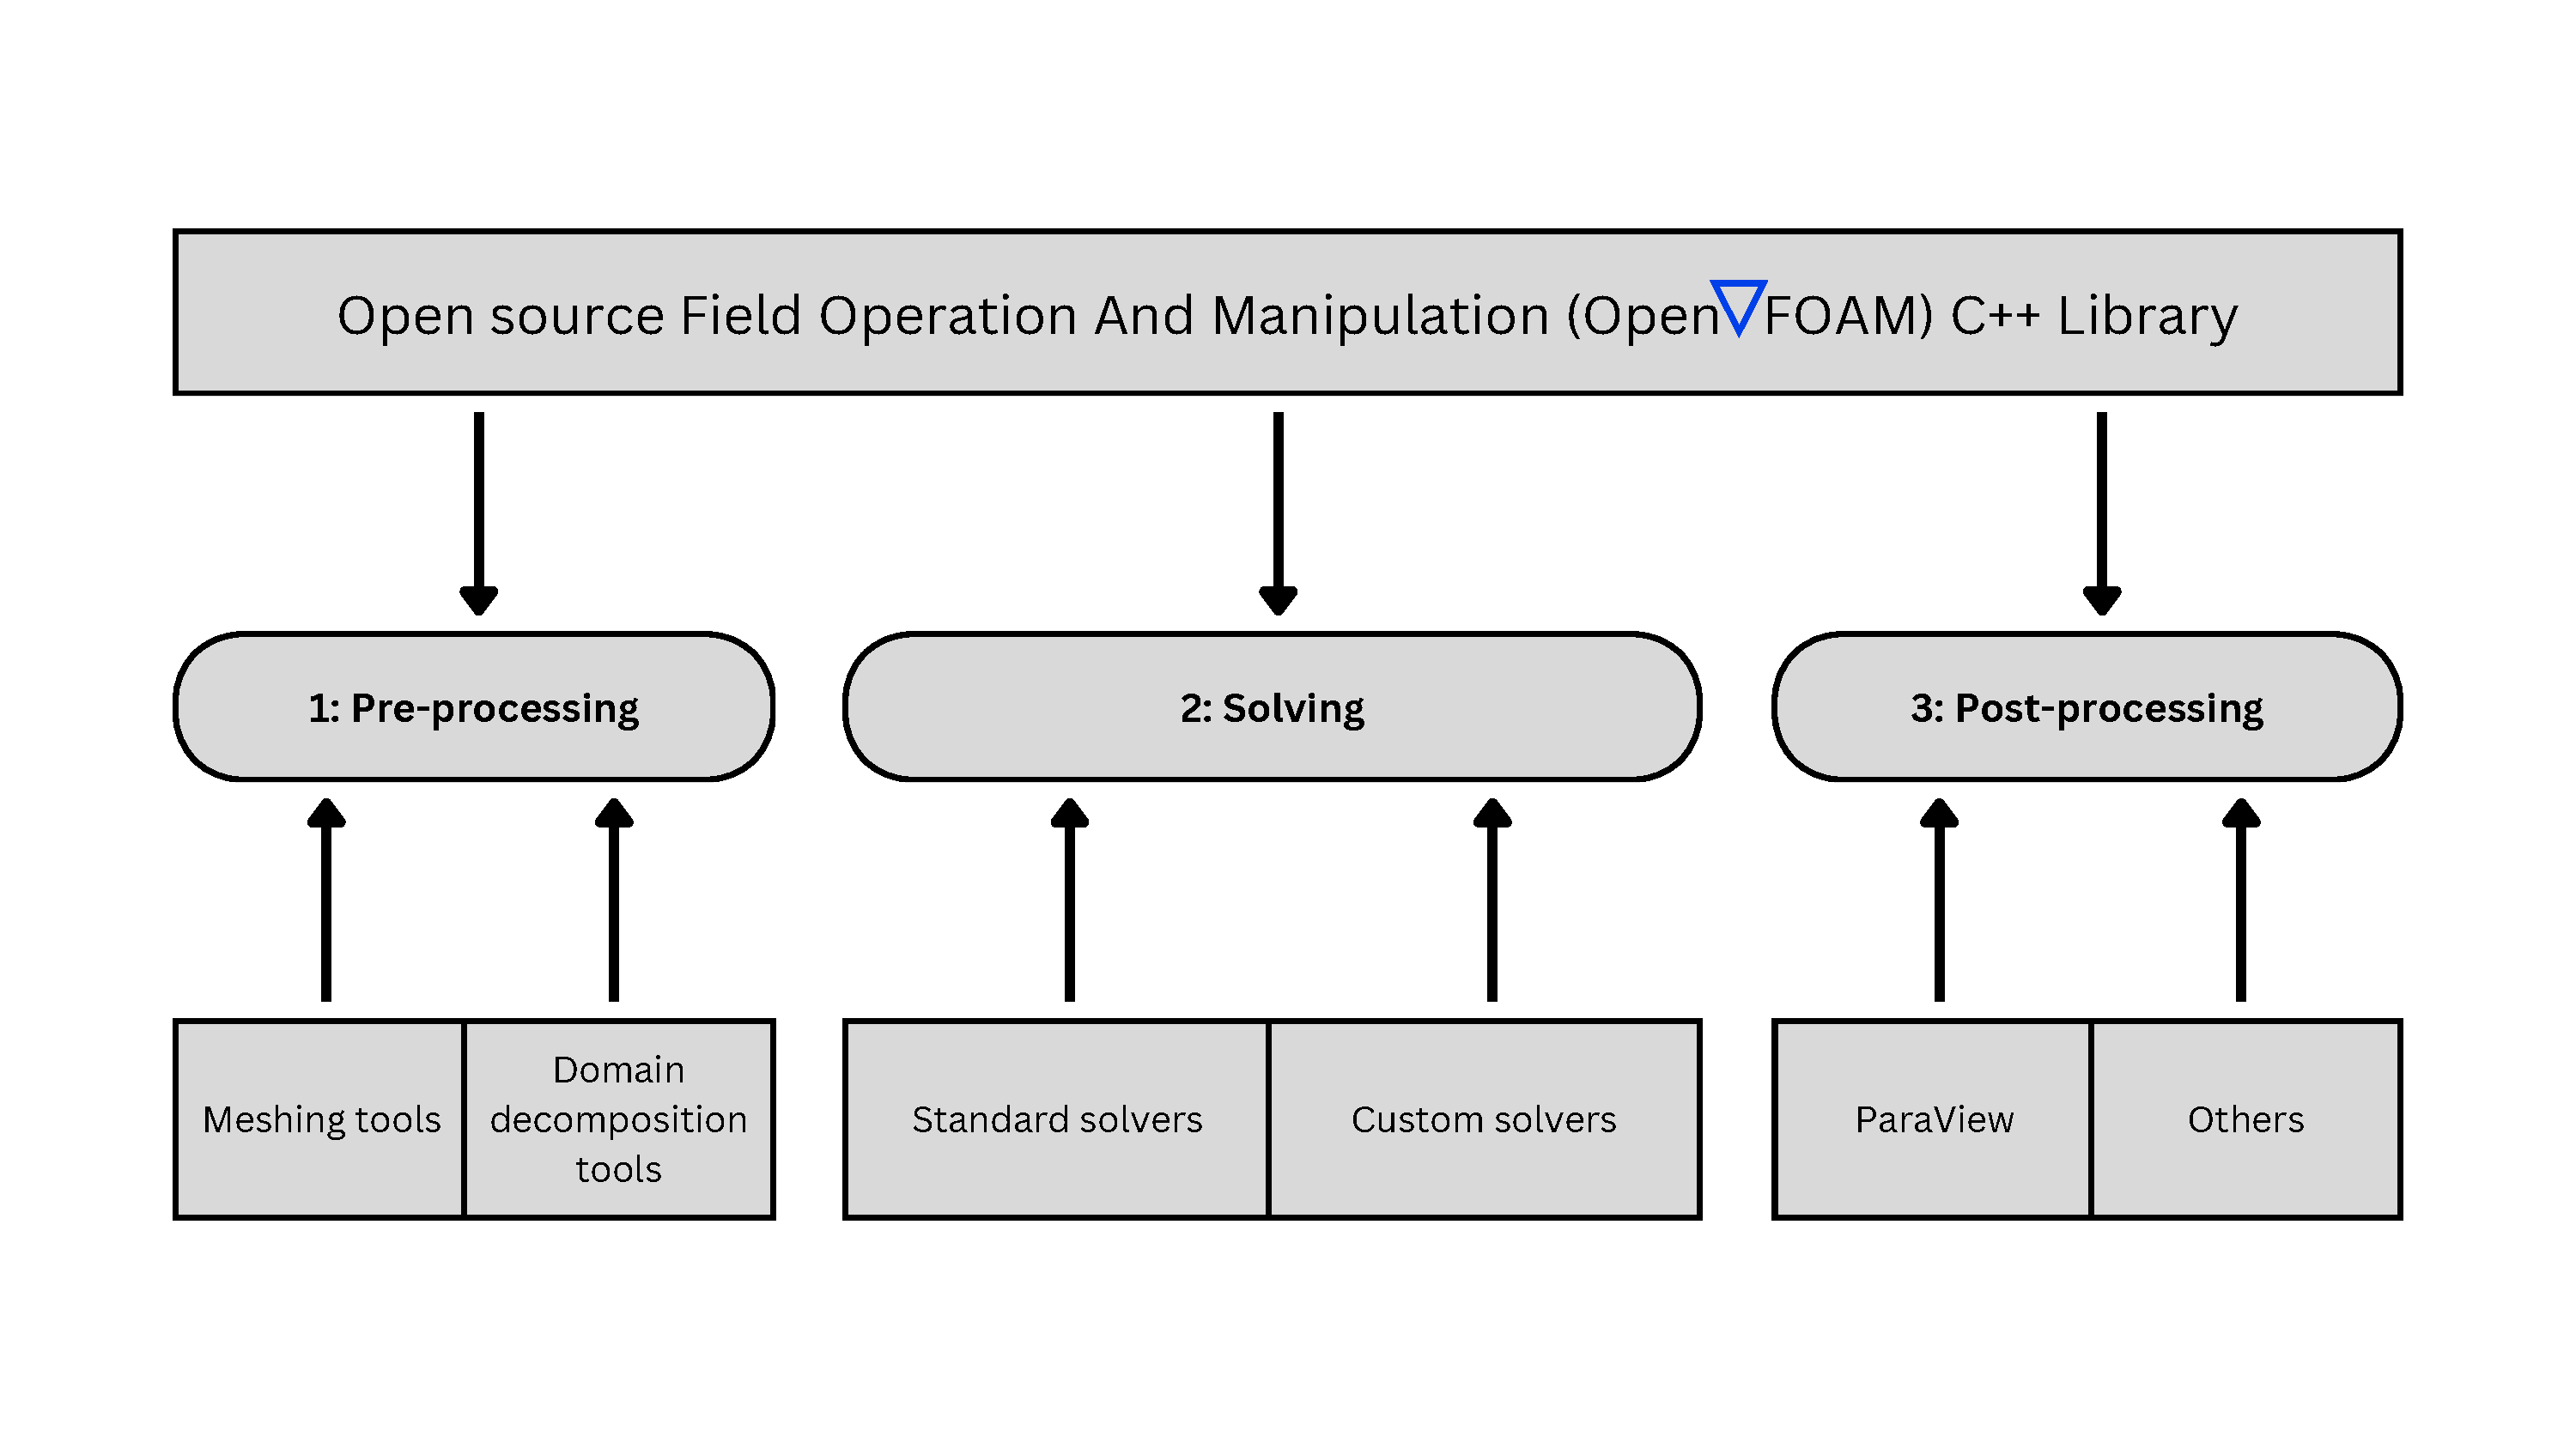
\includegraphics[width=1\linewidth]{Figures/OpenFOAM_structure}
		\caption{Overview of the OpenFOAM structure.}
		\label{OpenFOAM_structure}
	\end{figure}
	
	\noindent Figure \ref{OpenFOAM_directory_structure} shows the basic directory structure of an OpenFOAM standard case, including the essential files required to execute an application: 
	
	\begin{itemize}%[leftmargin=1]
		\item 
		\textbf{\textit{0} directory}: this is the first of the time directories required by the solver to start the simulation. In this directory, the initial condition and the boundary conditions for each physical quantity of the simulation (e.g. pressure ($p$), velocity ($U$) and temperature ($T$)) are specified.
		\item
		\textbf{\textit{constant} directory}: this folder contains the \say{polyMesh} folder where all the mesh data and the simulation boundary conditions are stored. It also contains all the properties needed to the solver, for instance the \say{thermophysicalProperties} file that specifies the thermodynamic and physical properties of the fluid or the \say{turbulenceProperties} file with the turbulence model used for the simulation.
		\item 
		\textbf{\textit{system} directory}: this folder contains the \say{controlDict} file where it is possible to define the settings of the simulation, for instance the used solver, the simulation time and the time-step. The methods for the discretization of the solved equations are specified in the \say{fvSchemes} file, while   the solvers for the discretized equations are specified in the \say{fvSolutions} file. A special mention goes to the \say{\textit{blockMesh}} utility command which creates parametric meshes with grading and curved edges. The mesh is generated from a dictionary file named blockMeshDict located in the \textit{system} directory. \say{\textit{blockMesh}} reads this dictionary, generates the mesh and writes out the mesh data files (boundary, faces, neighbour, owner and points) in the \say{polyMesh} folder, inside \say{constant}. Moreover, depending on the case problem, other files can be included in the system directory, for instance the \say{decomposeParDict} file to decompose the domain simulation into several processors such to run the simulation in parallel.
	\end{itemize}
	
	\noindent For the sake of completeness, we will describe the type of files inside the \say{polyMesh} folder. As been said above, the polyMesh subdirectory contains the followin files:
	
	\begin{itemize}
		\item \textbf{boundary}: the file boundary lists the boundaries of the domain, with the faces f each boundary type referred to as a patch and assigned a name. The type of each boundary patch (type) is declared along with its number of faces (nFaces) and the starting face (startFace),which refers to the index of the first face in the list;
		\item \textbf{faces}: the file faces represents a list of faces, with each face described by a list of indices to vertices in the points list where the first entry in the list represents face 0, the second entry represents face 1 and so on;
		\item \textbf{neighbour}: it is a list of neighbour cell labels. The number of neighbours is basically equal  the number of interior faces;
		\item \textbf{owner}: the file owner is a list in which the owner of faces are stored. The position of the owner in the list refers to the face it belongs to. The number of owners is equal to the total number of faces (interior + boundary faces);
		\item \textbf{points}: the file points is a list of vector denoting the cell vertices, with vertex 0 being the first vector in the list, vertex 1 the second vector, etc. 
	\end{itemize}
	
	\begin{figure}
		\centering
		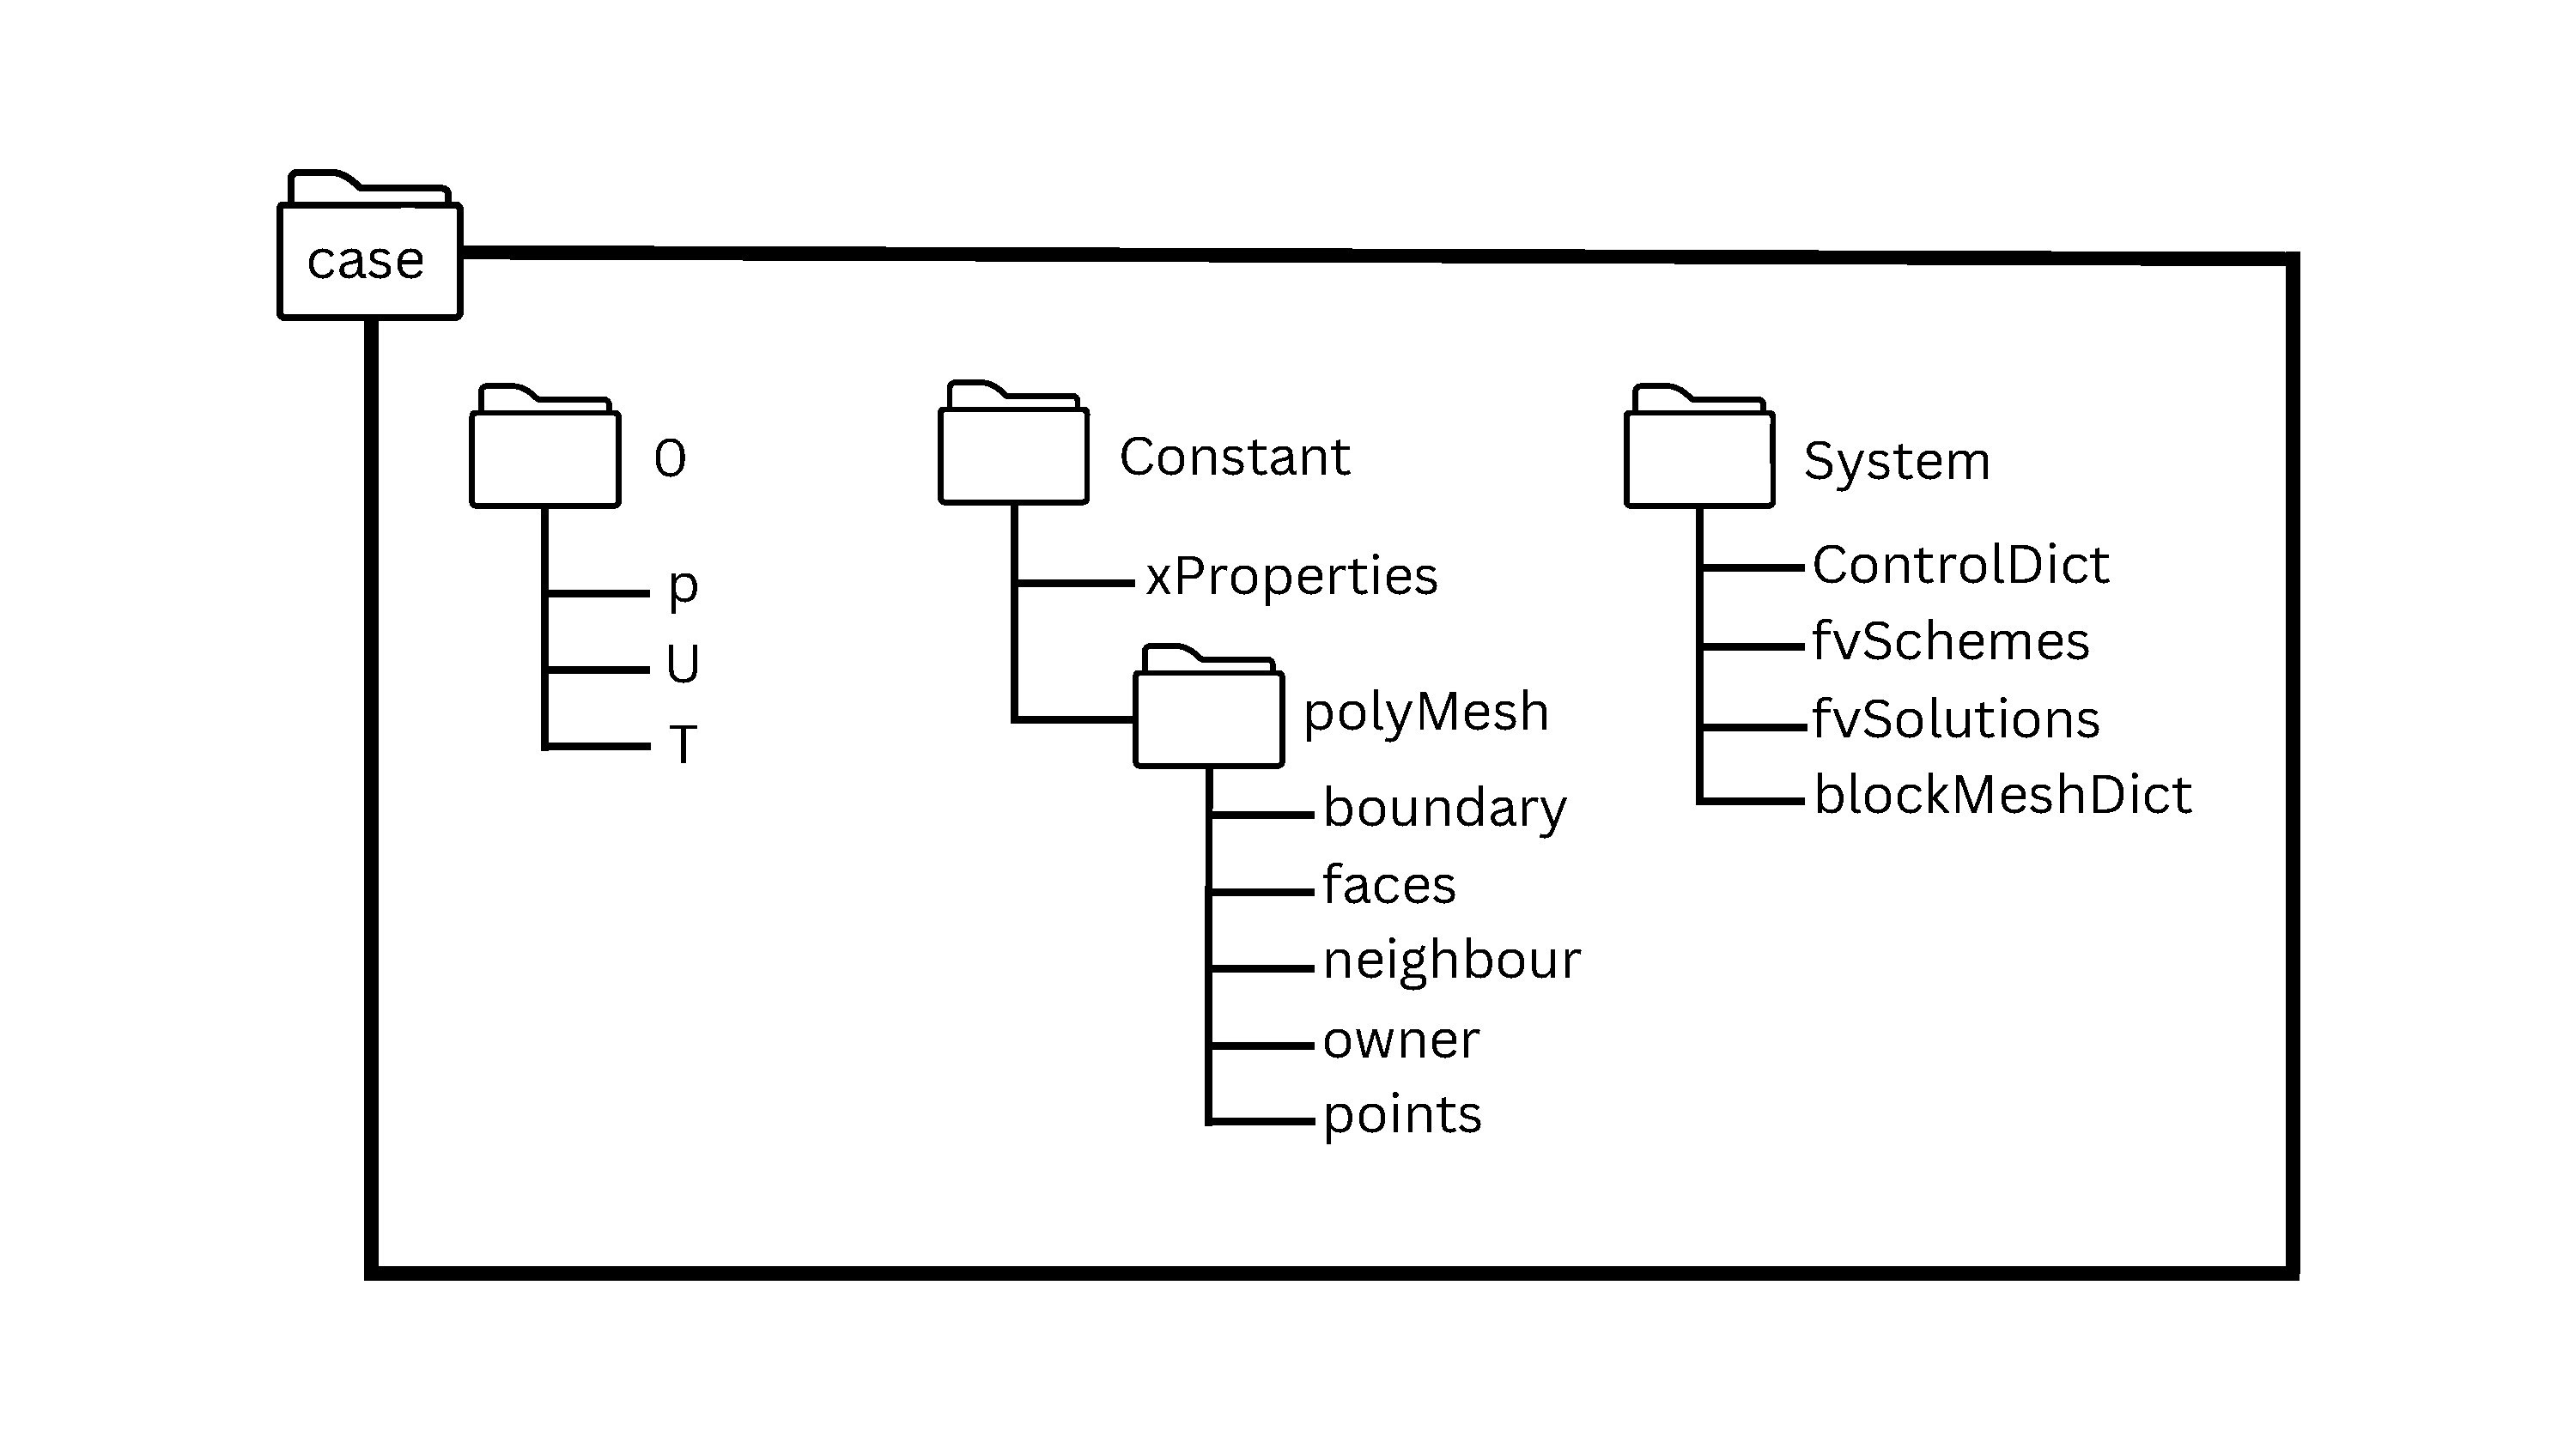
\includegraphics[origin=c, width=0.75 \linewidth]{Figures/Case_directory_structure}
		\caption{Case directory structure.}
		\label{OpenFOAM_directory_structure}
	\end{figure}
	
	\noindent OpenFOAM can handle continuum mechanics problems resolving Partial Differencial Equations (PDEs) using the Finite Volume Method over arbitrary polyhedric meshes.
	
	\section{The Finite Volume Method}
	
	The Finite Volume Method (FVM)\citep{ferziger2019computational} is a numerical technique that transforms the
	partial differential equations representing conservation laws over differential volumes into discrete algebraic equations over finite volumes (or elements or cells).
 	It gains popularity in CFD for being highly flexible as a discretization method. Even though it was preceded for many years by the Finite Difference (FD)\cite{crank1947practical} and Finite Element Method (FEM)\cite{clough1990original}, the FVM played a defining role in advancing the simulation of fluid flow problems and associated transport phenomena. This prominence arose from the groundbreaking work of the Computational Fluid Dynamics (CFD) group at Imperial College in the early 70s, led by Professor Spalding. Influential contributors such as \citet{gosman1969heat} and \citet{runchal1969numerical} among others, made significant strides in developing methods that shaped the field. 
	\\
	The FVM used in OpenFOAM follows the cell-centered logic, which is currently the most popular type of variable arrangement. This practice stores the quantities and the variables at the centroids of grid cells. More precisely, the solution domain is divided into a finite number of adjoining control volumes ($V_{p}$), and conservation equations are applied individually to each $V_{p}$. The computational node $P$ is positioned at the centroid of each control volume, where variable values are calculated. To estimate values at the surfaces of each $V_{p}$, interpolation is used to express these in terms of the nodal values located at the control volumes centers. Another way of looking at this is that FVM uses a volume integral formulation of the problem with a finite partitioning set of volumes to discretize the equations. The finite volume methods flexibility allows it to work with any type of grid, making it ideal for handling complex geometries. Additionally, the FVM ensures quantities conservation by construction, as long as the surface integrals, which represent convective and diffusive fluxes, are consistent across shared $V_{p}$ boundaries. This means that this method is inherently designed to conserve key physical quantities—such as mass, momentum, and energy—within the solution domain. This conservation property is built into the method itself, ensuring that the total amount of a conserved quantity entering or leaving a control volume (CV) equals the net accumulation or depletion of that quantity within the CV. \\
	Here we consider the general transport equation in its integral form:
	
	\begin{equation} 
		\int_{V_{p}}{{\dfrac{\partial{\rho \phi}}{\partial{t}}}}\ \mathrm{d}V + \int_{V_{p}}{\nabla \cdot (\rho u \phi)}\ \mathrm{d}V - \int_{V_{p}}{\nabla \cdot (\rho \Gamma_{\phi} \nabla\phi)}\ \mathrm{d}V = \int_{V_{p}}{S_{\phi}(\phi)}\ \mathrm{d}V
		\label{Transport equation}
	\end{equation}
	\\
	The first term of the equation \ref{Transport equation} is the integral over the volume $V_{P}$ of the temporal derivative of the product of the density $\rho$ and the generic transported quantity $\phi$, the second term is the integral of the convective term (that is the product of the density $\rho$, the velocity field $u$ and the transported quantity $\phi$), the third is the integral of the diffusion term and the last is the integral of the source term. 
	Now, let us recall the Gauss theorem which states that the outward flux of a vector field through a closed surface is equal to the volume integral of the divergence over the region inside the surface:
	
	\begin{equation}
		\int_{V}{\nabla \cdot u \ }\mathrm{d}V = \int_{\partial{V}}{u \cdot n \ \mathrm{d}S}
		\label{Gauss theorem}
	\end{equation}
	\\
	where $\partial{V}$ is a closed surface bounding the generic control volume $V$ and $\mathrm{d}S$ represents an infinitesimal surface element with associated normal $\hat{n}$ pointing outwards of the surface $\partial{V}$.
	\\
	If we use the Gauss theorem to convert the volume integrals into surface integrals, that is using equation \ref{Gauss theorem} into equation \ref{Transport equation}, we obtain the following equation
	
	\begin{equation}
		\dfrac{\partial}{\partial{t}}\int_{V_{p}}{{(\rho \phi)}}\ \mathrm{d}V + \int_{\partial{V_{p}}}{ (\rho u \phi)\cdot n}\ \mathrm{d}S - \int_{V_{p}}{(\rho \Gamma_{\phi} \nabla\phi)\cdot n}\ \mathrm{d}S = \int_{V_{p}}{S_{\phi}(\phi)}\ \mathrm{d}V
		\label{Transport equation_2}
	\end{equation}
	\\
	Now we can take a step further and move from the continuous domain to the discrete domain for each term.
	\\ 
	For the convective term we have:
	
	\begin{equation}
		\int_{\partial{V_{p}}}{(\rho u \phi)} \cdot n \ \mathrm{d}S = \sum_{f}\int_{f}{(\rho u \phi)_{f}} \cdot n \ dS \simeq \sum_{f} (\overline{\rho u \phi})_{f} \cdot n \ S_{f} = \sum_{f} (\rho u \phi)_{f} \cdot n \ S_{f}
		\label{convective discrete}
	\end{equation}
	\\
	For the diffusive term we have:
	
	\begin{equation}
		\begin{aligned}
			\int_{\partial{V_{p}}}{(\rho \Gamma_{\phi} \nabla \phi)} \cdot n\ \mathrm{d}S = \\ 
			\sum_{f}\int_{f}{(\rho \Gamma_{\phi} \nabla \phi)_{f}} \cdot n\ \mathrm{d}S \simeq \sum_{f} (\overline{\rho \Gamma_{\phi} \nabla \phi})_{f} \cdot n \ S_{f} =\\
			\sum_{f} (\rho \Gamma_{\phi} \nabla \phi)_{f} \cdot \hat{n} \ S_{f}
		\label{diffusive discrete}
	\end{aligned} 
	\end{equation}
	\\
	where, in the third term of both the convective and diffusive parts, we have approximated the integrant by means of the mid point rule, which is second order accurate.
	\\
	For the source term we have:
	
	\begin{equation}
		\int_{V_{p}}{(\phi) S_{\phi}} \ \mathrm{d}V = S_{c}V_{P} + S_{p}V_{P}\phi_{P}
		\label{source discrete}
	\end{equation}	
	\\
	This approximation is exact if $S_{\phi}$ is either constant or varies linearly with the control volume; otherwise is second order accurate. $S_{c}$ is the constant part of the source term and $S_{P}$ is the non-linear part.
	\\
	Using equations \ref{convective discrete}, \ref{diffusive discrete} and \ref{source discrete} into equation \ref{Transport equation_2}, we obtain the following  semi-discrete transport equation:
	
	\begin{equation}
		\dfrac{\partial}{\partial{t}}\int_{V_{p}}{{(\rho \phi)}}\ dV + \sum_{f} (\rho u \phi)_{f} \cdot n \ S_{f} - \sum_{f} (\rho \Gamma_{\phi} \nabla \phi)_{f} \cdot n \ S_{f} = S_{c}V_{P} + S_{p}V_{P}\phi_{P}
		\label{Discrete transport equation_2}
	\end{equation}
	\\
	where $(\rho u \phi)_{f} \cdot n \ S_{f} = F^{C}$ is the convective flux and $(\rho \Gamma_{\phi} \nabla \phi)_{f} \cdot n \ S_{f}=F^{D}$is the diffusive flux.
	All of this is necessary to transform the governing partial differential equations into a set of algebraic equations, one for each element in the computational domain. These algebraic equations are then assembled into a global matrix and vectors that can be expressed in the form 
	
	\begin{equation}
		A x = b
		\label{matrix form}
	\end{equation}
	\\
	where $A$ is the $N \times N$ coefficient matrix, $x$ is the unknown $N$ vector variable which is defined at each interior element and at the boundary of the computational domain, and $b$ is the vector of dimension $N$ of the known variables. One of the main advantages of the Finite Volume Method is that the techniques to solve the algebraic system of equations are independent of the discretization method, and represent the various trajectories that can be followed to obtain a solution. 
	It is important to recall that the variables are computed and stored at the centroid $P$ of the control volumes. This means that the face values in the convective and diffusive fluxes have to be computed by some form of interpolation from the centroid of the control volume at both sides of the face $f$.
	
	\section{Interpolation Schemes}
	
	Interpolation schemes are numerical methods used to estimate values at intermediate points within a discrete set of data or across a continuous domain. Interpolation methods range from simple approaches like linear and polynomial interpolation to more complex schemes designed to handle challenges like sharp gradients or discontinuities in data, which are common in physical simulations and engineering applications. Employing the Finite Volume Method (FVM), the partial differential equations are transformed into algebraic equations by integrating over discrete control volumes in the computational domain. This transformation requires both spatial and temporal discretization to approximate the solution within each control volume and over successive time steps.
	
	\subsection{Spatial Discretization}
	Spatial discretization is a critical component of the Finite Volume Method (FVM) when solving the Navier-Stokes equations, as it directly influences the accuracy, stability, and efficiency of the solution. In FVM, spatial discretization involves dividing the computational domain into a finite number of control volumes and approximating flow quantities and their derivatives, such as velocity and pressure, at the boundaries of these control volumes. When a the domain is two dimensional (2D) the boundaries of the control volumes is the edge of the cell and when it is three dimensional (3D) the boundary is the face of the control volume. This process enables the transformation of the continuous partial differential equations into discrete algebraic equations, which are then solved numerically.
	\\
	For high-speed flows, effective spatial discretization is essential. In such flows, sharp gradients in velocity, temperature, and pressure are common, especially near shock waves, boundary layers, and regions of rapid compression and expansion. Accurately capturing these gradients without introducing numerical errors, such as diffusion oscillations, is essential for a realistic representation of the flow field. As discussed in the review on numerical methods for high-speed flows (\citet{Pirozzoli2011}), the interpolation schemes chosen for spatial discretization play a decisive role in balancing stability and accuracy under these challenging conditions.
	\\
	In the context of the Navier-Stokes equations, spatial discretization must be applied to three terms: convective, diffusive, and gradient term. Each one requires distinct handling due to the different physical phenomena they represent. In the following paragraphs each term will be described.
	
	\subsubsection{Convective Terms}
	
	Convective terms model the transport of fluid properties, such as scalar quantities, momentum or energy, because they model the bulk motion of the flow. These terms are particularly dominant in high-speed flows, where their nonlinear nature often leads to steep gradients and discontinuities, such as shocks and expansions. Accurate resolution of these gradients is critical for capturing the essential features of compressible flows, but it poses significant numerical challenges. In fact, if the choosen discretization results inadequate, it can lead to excessive numerical diffusion with a consequent unphysical oscillations result that compromise solution fidelity.	 
	Several discretization schemes have been developed in the past decades and they are currently employed for convective terms. For instance, the \textit{Upwind Scheme}, which selects values from the upstream cell, is robust and stable, making it a popular choice for high-speed flows. However, its inherent numerical diffusion can obscure sharp gradients, making it less suitable for applications requiring high accuracy. In contrast, the \textit{Central Differencing Scheme} (CDS) achieves higher accuracy by averaging values from adjacent cells. While effective in resolving smooth gradients, CDS is prone to numerical oscillations in flows dominated by convection, limiting its applicability in scenarios involving strong discontinuities.
	\\
	To address these limitations, higher-order schemes, such as \textit{QUICK} (Quadratic Upstream Interpolation for Convective Kinematics)\cite{leonard1979stable} and \textit{MUSCL} (Monotonic Upstream-Centered Schemes for Conservation Laws)\cite{toro2013riemann}, have been developed. These methods incorporate information from multiple neighboring cells to achieve greater accuracy and reduce numerical diffusion. QUICK is particularly effective in capturing smooth gradients, while MUSCL, with its flux-limiting approach, is better suited for problems with shocks and steep gradients. Another robust and widely used  numerical scheme in CFD is the Advection Upwind Splitting Method (AUSM)\cite{LIOU_AUSM}, used for solving compressible flow problems. More precisely, it exist a rich AUSM family with  integrating enhancements that improve accuracy, stability, and efficiency, particularly in the presence of shock waves, contact discontinuities, and low-Mach-number flows. For example $AUSM^+-up$ achieves this by employing a blend of pressure-based and velocity-based flux splitting techniques while incorporating additional terms to stabilize pressure and velocity interactions. These refinements make $AUSM^+-up$ especially suitable for a broad spectrum of aerospace applications, from high-speed aerodynamics to propulsion system modeling, where precision in capturing complex flow physics is critical.
	The AUSM formulation is described herein in section \ref{AUSMsection}. The choice of the most suitable scheme in high-speed flows is a key aspect as it must balance accuracy and stability to handle the complex interplay of sharp gradients and nonlinearities. 
	\\
	The development of hybrid and adaptive schemes, which dynamically combine the strengths of multiple approaches, is an active area of research. These methods aim to achieve a balance between numerical diffusion and oscillations, making them particularly useful in simulations involving shocks, turbulence, and other complex flow features.
	
	\subsubsection{Diffusive Terms}
	Diffusion terms represent molecular diffusion processes, including viscosity and thermal conduction, which are governed by the physical properties of the fluid. Unlike convective terms, diffusion terms are generally linear, making their numerical treatment more straightforward. They are typically discretized using the \textit{Central Differencing Scheme} (CDS), which provides second-order accuracy on uniform grids. The symmetry and non-oscillatory nature of central differencing ensure stable and accurate approximation of diffusive fluxes, making it a preferred choice for the Finite Volume Method (FVM) employed in solvers such as OpenFOAM.
	\\
	Although diffusion effects are often small compared to convection in high-speed flows, their accurate representation is critical in regions where viscous effects dominate, such as boundary layers and shock-boundary layer interactions. In these areas, diffusion terms govern the transfer of momentum and energy at small scales, influencing key flow characteristics like skin friction and heat transfer. Proper discretization of these terms is essential for capturing the dynamics of shear layers, turbulence, and thermal gradients.
	\\
	Recent advances in adaptive and high-order schemes have further improved the treatment of diffusion terms, especially in simulations involving non-uniform grids or complex geometries. These methods help mitigate errors arising from grid irregularities while preserving accuracy and computational efficiency, ensuring reliable results in high-fidelity simulations.
	
	
	\subsubsection{Gradient Terms}
	
	Gradient terms, such as those arising in pressure gradient calculations, play a crucial role in fluid dynamics as they govern the acceleration and deceleration of the flow. Accurate computation of these terms is essential for capturing the dynamics of pressure-driven flows, particularly in regions with sharp pressure changes or discontinuities, such as shock waves or boundary layer separations. In computational fluid dynamics, gradient terms are typically discretized using \textit{linear central differencing}, a scheme that provides second-order accuracy on structured grids. This method is widely adopted in solvers like OpenFOAM due to its simplicity, stability, and effectiveness in regions of smooth flow.
	\\
	While \textit{linear central differencing} is effective for smooth flows, its reliance on grid uniformity can pose challenges in complex geometries or highly unstructured grids, where the accuracy of gradient calculations may deteriorate. To address these issues, advanced methods such as \textit{least squares gradient reconstruction} and \textit{weighted averaging techniques} have been developed. These approaches improve robustness and accuracy in non-uniform meshes, making them suitable for high-fidelity simulations in complex domains. 
	\\
	In high-speed flows, the accurate representation of pressure gradients is particularly critical, as errors in these terms can propagate through the solution, impacting the prediction of shock structures, expansion fans, and other key flow features. Therefore, careful selection and implementation of gradient discretization schemes are integral to achieving reliable and precise CFD results.
	
	\subsection{Flux Splitting Schemes}
	
	The story of flux splitting schemes begins in the late 1970s, when researchers were grappling with the challenge of accurately capturing shock waves and other discontinuities in compressible flow simulations. The key insight was that by splitting the flux terms into positive and negative components based on wave propagation directions, one could better handle these challenging flow features.The Godunov scheme, introduced by Sergei Godunov in 1959, represented a revolutionary approach to numerical fluid dynamics. This method solves the exact or approximate Riemann problem at cell interfaces, considering the flow as a series of interacting waves. The scheme's ability to naturally capture shock waves and maintain conservation properties made it a cornerstone of modern CFD, though its computational cost was initially seen as a drawback. Building on these foundations, the Total Variation Diminishing (TVD) scheme emerged in 1983 through the work of \citet{HARTEN1983}. TVD schemes introduced the crucial concept of limiting the numerical solution's total variation to prevent spurious oscillations near discontinuities. This advancement addressed a key limitation of earlier high-order methods which often produced unphysical oscillations near shock waves. The TVD property ensures that the numerical solution remains stable and physically meaningful, making these schemes particularly valuable for compressible flow calculations.
	One further advancement in the flux splitting domain is the development of the Advection Upwind Splitting Method (AUSM) and its subsequent iterations: AUSM+ and AUSM+-up. The AUSM (Advection Upstream Splitting Method) scheme, developed by \citet{LIOU_AUSM} in 1993, represents a more sophisticated approach to flux splitting. It cleverly separates the convective and pressure terms in the flux vector, treating them differently based on their physical nature. The scheme combines the accuracy of flux-difference splitting methods like Godunov's with the computational efficiency of flux-vector splitting approaches. What makes AUSM particularly noteworthy is its ability to accurately capture both inviscid and viscous flow features while maintaining excellent robustness and efficiency. These three schemes are interconnected through their progressive refinement of flux splitting concepts. While Godunov's scheme laid the theoretical groundwork with its wave-based approach, TVD schemes added the crucial property of solution stability, and AUSM brought everything together with a physically motivated splitting that balanced accuracy and computational efficiency. Together, they represent key milestones in the development of modern computational fluid dynamics methods.\\
	
	\noindent This section provides a comprehensive overview of these flux splitting schemes, their numerical algorithms, and their significance in addressing the challenges of all-speed flows.
	
	\subsubsection{Upwind methods}
	
	The upwinding approach, widely adopted within the gas dynamics community, is founded on the principle that the solutions of the Euler equations propagate along characteristic lines. Consequently, a stable numerical method must ensure that information is propagated in the same characteristic directions (\citet{MORETTI1979191}). Within the finite difference (FD) framework, the conventional methodology, known as flux vector splitting (\citet{STEGER1981263}), involves decomposing the flux function into positive and negative components:
	
	\begin{equation}
		f(u) = f^+(u) + f^-(u),
	\end{equation}
	\\
	where $f^+(u)$ and $f^-(u)$ correspond to non-negative and non-positive propagation velocities, respectively, i.e.,
	
	\begin{equation}
		\dfrac{\mathrm{d}f^+}{\mathrm{d}u} \geq 0 \quad \text{and} \quad \dfrac{\mathrm{d}f^-}{\mathrm{d}u} \leq 0.
	\end{equation}
	\\
	These components are discretized using left- and right-biased approximations to maintain linear stability.
	
	In the finite volume (FV) framework, upwinding is typically achieved via the flux difference splitting approach, also referred to as the Godunov method. Considering the one-dimensional (1D) scalar conservation law:
	
	\begin{equation}
		\dfrac{\partial u}{\partial t} + a(u) \dfrac{\partial u}{\partial x} = 0
		\label{conservationlaw}
	\end{equation}
	\\
	which is used as a prototype for the development of numerical methods for hyperbolic equations, we can derive its FV semi-discretization form as follows:
	
	\begin{equation}
		\dfrac{\partial \overline{u}_j}{\partial t} = \dfrac{1}{h}(f(u_{j+1/2}) - f(u_{j-1/2})),
	\end{equation}
	\\
	where $\overline{u}_j(t) = 1/h \int_{x_{j-1/2}}^{x_{j+1/2}} u(x,t) dx$ is the spacial average of the approximate solution over the cell $I_j = (x_{j-1/2},x_{j+1/2})$, a suitable reconstruction operator is used to determine approximate left and right states at the cell interfaces, $u_{j+1/2}^{\pm}$, and the interface flux $f(u_{j+1/2})$ is replaced with the numerical flux resulting from an exact (or approximate) Riemann solver, formally $\hat{f}_{j+1/2} = \textit{R}(u_{j+1/2}^{-},u_{j+1/2}^{+})$. For example, Roe's approximate Riemann solver prescribes 
	
	\begin{equation}
		\begin{aligned}
			\textit{R}(u_{j+1/2}^{-},u_{j+1/2}^{+}) = \dfrac{1}{2}(f(u_{j+1/2}^{-})+f(u_{j+1/2}^{+}))+\\
			-\dfrac{|a_{j+1/2}|}{2}(u_{j+1/2}^{+} - u_{j+1/2}^{-})
		\end{aligned}
	\end{equation}
	\\
	where $a_{j+1/2}$ is the characteristic speed associated with the intermediate state and defined as
	
	\begin{equation}
		a_{j+1/2}=(f(u_{j+1/2}^+)-f(u_{j+1/2}^-))/(u_{j+1/2}^{+}-u_{j+1/2}^{-}).
	\end{equation}
	\\
	In Godunov's original formulation, piece-wise constant reconstructions were assumed, leading to the general first-order flux
	
	\begin{equation}
		\hat{f}_{j+1/2} = \textit{R}(\overline{u}_{j},\overline{u}_{j+1})
	\end{equation}
	\\
	Upwinding has the main effect of damping the Fourier modes with the highest supported
	wave numbers, with a subsequent stabilizing effect on the numerical solution.
	
	\subsection{The AUSM Schemes}
	\label{AUSMsection}
	
	The AUSM (Advection Upstream Splitting Method) scheme is a family of numerical schemes used in computational fluid dynamics (CFD) to solve compressible flow problems. Developed to enhance the accuracy and robustness of numerical simulations, the AUSM scheme efficiently handles shock waves, contact discontinuities, and smooth flow regions by carefully splitting the convective and pressure terms in the flux computation. Over time, various improved versions, such as AUSM+, AUSM+-up, and others, have been introduced to address stability and accuracy issues in high-speed flows. These schemes are widely applied in aerospace, automotive, and energy industries for simulating supersonic and transonic flows with high fidelity.
	
	\subsubsection{The AUSM Scheme}
	
	The original AUSM scheme, introduced by \citet{LIOU_AUSM} in their seminal paper \textit{“A New Flux Splitting Scheme”}, marked a significant departure from earlier flux vector and flux difference splitting methods. The key innovation of AUSM lies in its decomposition of fluxes into convective and pressure components, each treated separately to align with their respective physical characteristics.
	
	\subsubsection*{Numerical Formulation}
	
	Considering the two-dimensional system of Euler equation for perfect gas:
	
	\begin{equation}
		\dfrac{\partial{U}}{\partial{t}} + \dfrac{\partial{F}}{\partial{x}} +
		\dfrac{\partial{G}}{\partial{y}} = 0
	\end{equation}
	\\
	where the velocity field is 
	
	\begin{equation}
		U =
		\begin{pmatrix}
			\rho    \\
			\rho u  \\
			\rho v  \\
			\rho E
		\end{pmatrix},
	\end{equation}
	\\
	the inviscid fluxes are 
	
	\begin{equation}
		F =
		\begin{pmatrix}
			\rho u       \\
			\rho u^2 + p \\
			\rho uv      \\
			\rho u H
		\end{pmatrix}, \
		G =
		\begin{pmatrix}
			\rho u       \\
			\rho vu		 \\
			\rho v^2 + p \\
			\rho v H
		\end{pmatrix},
	\end{equation}
	\\
	and the specific total energy is $E = e +1/2(u^2+v2) = H -p/\rho$.	
	The AUSM scheme splits the inviscid flux $F$ into two components:
	
	\begin{equation}	
		\mathbf{F} = \mathbf{F^c} + \mathbf{F^p} = 
		\begin{pmatrix}
			\rho    \\	
			\rho u  \\
			\rho v  \\
			\rho H
		\end{pmatrix} u
		+
		\begin{pmatrix}
			0 \\
			p \\
			0 \\
			0
		\end{pmatrix},
	\end{equation}
	\\
	where $F_c$ represents the convective flux, and $F_p$ represents the pressure flux. The convective terms can now be considered as passive scalar quantities convected by a suitably defined velocity $u$ at the cell interface. On the other hand, the pressure flux terms are governed by the acustic wave speeds.The two components are discretized separately and at an interface $L<\dfrac{1}{2}<R$, the convective terms can be written as function of the Mach number $M$, ensuring upwinding to handle advection accurately:
	
	\begin{equation}
		F_{1/2}^c = M_{1/2}
		\begin{pmatrix}
			\rho a 	 \\
			\rho au  \\
			\rho av  \\
			\rho aH
		\end{pmatrix}_{L/R},
	\end{equation}
	\\
	where $(M_{1/2} \simeq M_L^+ +M_R^-)$ is the value of the split Mach number at the interface (red line in figure \ref{cells}) and $a$ is the speed of sound. Various ways of defining the split Mach number exist, for instance the Van Leer\citep{van1982} splitting:
	
	\begin{equation}
		M^{\pm} = 
		\begin{cases}
			\pm\dfrac{1}{4}(M \pm 1)^2  \hspace{10 mm} if \hspace{2 mm} |M| \leq 1;\\
			\dfrac{1}{2} (M \pm |M| ),  \hspace{10 mm} if \hspace{2 mm} otherwise
		\end{cases}
	\end{equation}	
	\\
	where $M_L^+$ is the value of the left contribution of the Mach number and $M_R^-$ is the value of the right contribution of the Mach number. Also 
	
	\begin{equation}
		(\cdot)_{L/R} = 
		\begin{cases}
			(\cdot)_L  \hspace{10 mm} if \hspace{2 mm} M_L^+ \geq M_R^-\\
			(\cdot)_R  \hspace{10 mm} if \hspace{2 mm} M_L^+ < M_R^-
		\end{cases}
	\end{equation}
	\\
	where L and R are the Left and Right side of two adjacent cells respectively, as in figure \ref{cells}.
	
	\begin{figure}[t]
		\centering
		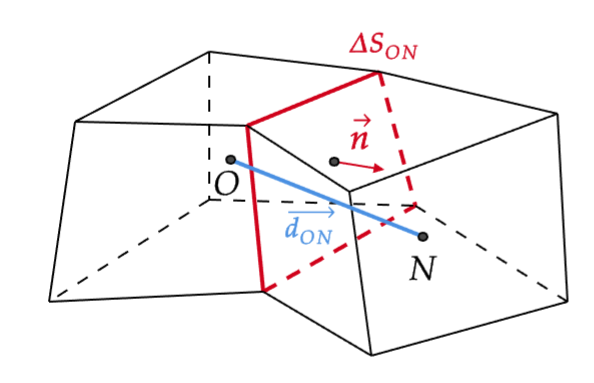
\includegraphics[width=0.5 \linewidth]{Figures/CELL3D.png}
		\caption[3D computational cell for numerical flux evaluation.]{Computational cell for numerical flux evaluation. \textcolor{red}{$\Delta S_{ON}$} represents the interface between the owner cell O and the neighboring cell N, with \textcolor{red}{$\vec{n}$} as the outward normal for O and \textcolor{Havelock Blue}{$\vec{d_{ON}}$} the distance between the cell centers O and N.}
		\label{cells}
	\end{figure} 
	\noindent The pressure flux is treated symmetrically to ensure accurate shock resolution and smooth transitions:
	\begin{equation}
		F_p = p_{1/2} = p_L^+ + p_R^-.
	\end{equation}
	\\
	The AUSM scheme is simple and computationally efficient, providing accurate shock capturing and robust performance for subsonic and supersonic flows, sometimes with better results than the ones obtained with the Roe scheme. However, it showed limitations in maintaining stability and accuracy for low-Mach-number flows.
	
	\subsubsection{The AUSM+ Scheme}
	
	To address the deficiencies of AUSM, particularly removing postshock overshoot and a glitch in the slowly moving shock problem, \citet{LIOU_AUSM+} introduced the $AUSM+$ scheme in the follow-up paper. This iteration improved robustness and extended the method’s applicability to a broader range of flow conditions. In fact, the scheme is capable of exactly capturing stationary shocks and contact discontinuities, it ensures that density remains positive, which is crucial for handling strong rarefaction and near-vacuum flows, and it significantly reduces the "carbuncle" issue that affects the Roe scheme and previous AUSM implementations in blunt-body simulations.
	The AUSM+ scheme improves the splitting approach by unifying the Mach number and velocity formulations while maintaining a simple structure, making it easily adaptable to other hyperbolic systems.  
	
	\subsubsection*{Algorithm}
	To implement the AUSM+ to a basic central-differencing code, it only requires the key interface quantities $(m_{j+1/2},p_{j+1/2})$ and unified numerical speed of sound $a_{j+1/2}$.  
	The Mach number is split to minimize numerical dissipation at low Mach numbers.
	
	\begin{equation}
		\begin{aligned}
			2m_{j+1/2} = (M_j +M_{j+1})-(\mathscr{M}_{j+1}^+ - \mathscr{M}_{j+1}^-)+\\
			+(\mathscr{M}_{j}^+ - \mathscr{M}_{j}^-)-\delta m_{j+1/2},
		\end{aligned}
	\end{equation}
	\\
	where
	
	\begin{equation}
		|\mathscr{M}|(M)= \mathscr{M}^+(M)-\mathscr{M}^-(M), 
	\end{equation}
	\begin{equation}
		\delta m = |\mathscr{M}|(M-{j+1})-|\mathscr{M}|(M_j) 
	\end{equation}
	\\
	and
	
	\begin{equation}
		|\mathscr{M}|(M) = 
		\begin{cases}
			|M|,\qquad \qquad \qquad \qquad \qquad \quad |M|\geq1\\
			\dfrac{1}{2}(M^2 +1)+2\beta(M^2-1)^2,\quad otherwise
		\end{cases}
	\end{equation}
	\\
	Since $|\mathscr{M}| >0 \forall M$, the absolute sign to $\mathscr{M}$ make sense. On the other hand $\Delta |\mathscr{P}|$ can be either positive or negative, depending on the sign of M:
	
	\begin{equation}
		|\mathscr{P}|(M) = 
		\begin{cases}
			sign(M), \qquad \qquad \qquad \qquad \qquad |M|\geq1\\
			\dfrac{M}{2}(3-M^2+4\alpha(M^2-1)^2), \hspace{5mm}   otherwise
		\end{cases}
	\end{equation}
	\\
	Here, the pressure flux is modified to ensure smooth transitions between subsonic and supersonic regimes. The pressure flux incorporates a blending function to adapt dynamically
	
	\begin{equation}
		2p_{j+1/2} = (p_j +p_{j+1})-\delta p_{j+1/2}
	\end{equation}
	\\
	where
	
	\begin{equation}
		\delta p_{j+1/2} = \Delta \mathscr{P}(M_{j+1})p_{j+1} - \Delta \mathscr{P} (M_{j})p_j 
	\end{equation}
	\\
	and
	
	\begin{equation}
		\Delta \mathscr{P}(M) = \mathscr{P}^+(M) - \mathscr{P}^-(M) 
	\end{equation}
	\\
	Once the quantities $(\delta p_{j+1/2},\delta m_{j+1/2})$ have been defined, the dissipative terms derived from the AUSM+ are ready to be added. Rewriting the AUSM+ flux in terms of the central-difference (CD) formula yields,
	
	\begin{equation}
		f_{j+1/2}^{AUSM^+} = f_{j+1/2}^{CD} + f_{j+1/2}^{vis} 
	\end{equation}
	\\
	where 
	\begin{equation}
		f_{j+1/2}^{vis} = f_{j+1/2}^C +f_{j+1/2}^P
	\end{equation}
	\\
	or, explicitly, the convection term is
	
	\begin{equation}
		\begin{aligned}
			f_{j+1/2}^C = - \dfrac{a_{j+1/2}}{2} \Big[\Big(\dfrac{1}{2}\delta m_{j+1/2}-|m_{j+1/2}|\Big)\Phi_j + \\
			+\Big(\dfrac{1}{2}\delta m_{j+1/2}+|m_{j+1/2}|\Big)\Phi_{j+1}\Big]
		\end{aligned}
	\end{equation}
	\\
	and the pressure term is
	
	\begin{equation}
		f_{j+1/2}^P = -\dfrac{1}{2}
		\begin{pmatrix}
			0 \\
			\delta p_{j+1/2}\\
			0
		\end{pmatrix}.
	\end{equation}
	\\
	This scheme improved stability and accuracy at low Mach numbers, enhanced shock and contact discontinuity resolution, and reduced dissipation for smooth flow regions.
	
	\subsubsection{The AUSM+-up Scheme}
	
	Recognizing the need for a unified framework capable of handling flows across all speeds, which could not be achieved with AUSM+, in 2006 \citet{LIOU_AUSM+-up} proposed the AUSM+-up scheme in \textit{“A Sequel to AUSM, Part II: AUSM+-up for All Speeds”}. As for its predecessors, this method integrates pressure-based and velocity-based splitting strategies, with more precise corrections that allowed the achieving of superior performances. In fact, the previous AUSM+ scheme had two critical deficiencies that affect compressible flow solvers, particularly when applied to low-speed flow predictions. These deficiencies manifest as two distinct yet interconnected problems: an intrinsic convergence instability and a fundamental inaccuracy in solution generation.
	The first issue originates at the continuum level, fundamentally tied to the governing equations' mathematical structure. This convergence challenge exists independently of the spatial discretization scheme employed, representing a deep-rooted numerical complexity. The second deficiency, however, is directly linked to the flux numerical scheme itself, offering a more tractable avenue for methodological intervention.
	Previous computational approaches, despite their practical successes, revealed significant limitations. The pressure split function exhibited a critical discontinuity at zero Mach number, necessitating arbitrary cut-off parameters that artificially constrained the method's applicability. Existing preconditioners relied on preset Mach number limitations, which fundamentally restricted the method's universal potential. The core objectives of the Liou's latest article are ambitious yet precise: to create a flux scheme that ensures convergence rates independent of Mach numbers in low-speed flows, maintains at least equivalent performance in other speed regimes, and preserves solution accuracy across the entire spectrum of flow conditions.
	
	\subsubsection*{Algorithm}
	The AUSM+-up scheme introduces two critical modifications:
	
	\begin{itemize}
		\item The pressure flux incorporates an additional dissipation term proportional to the pressure difference to stabilize low-Mach-number flows.
		\item 	The convective flux is enhanced by adding a pressure-difference-driven velocity correction, ensuring robustness across all speed regimes.
	\end{itemize} 
	
	\noindent The Mach number and speed of sound at the interface are defined as:
	
	\begin{equation}
		M_{L/R} = \dfrac{u_{L/R}}{a_{1/2}},
	\end{equation}
	\\
	where $a_{1/2}$ can be an average of $a_L$ and $a_R$. For multi-dimensional flows, $u = \mathbf{V} \cdot \mathbf{n}$, with $\mathbf{n}$ as the unit normal vector of the cell face under consideration.
	
	\noindent The following auxiliary quantities are computed:
	
	\begin{equation}
		\bar{M}^2 = \dfrac{u_L^2 + u_R^2}{2a_{1/2}^2},
	\end{equation}
	\\
	\begin{equation}
		M_o^2 = \min(1, \max(\bar{M}^2, M_1^2)),
	\end{equation}
	\\
	\begin{equation}
		f_a(M_o) = M_o (2 - M_o),
	\end{equation}
	\\
	where $f_a(M_o)$ is a scaling factor. \\
	
	\noindent Then, we can compute the mass flux and pressure fluxes as in \ref{massflux} and \ref{pressureflux}
	
	\begin{equation}
		\dot{m}_{1/2} = a_{1/2} M_{1/2} \begin{cases}
			q_L & \text{if } M_{1/2} > 0, \\
			q_R & \text{otherwise},
			\label{massflux}
		\end{cases}
	\end{equation}
	\\
	where $M_{1/2}$ is defined as:
	
	\begin{equation}
		M_{1/2} = M_+^{(4)}(M_L) + M_-^{(4)}(M_R) - \dfrac{K_p}{f_a} \max(1 - r \bar{M}^2, 0) \dfrac{p_R - p_L}{q_{1/2} a_{1/2}^2},
	\end{equation}
	\\
	with $q_{1/2} = \dfrac{q_L + q_R}{2}$.
	
	\begin{equation}
		\begin{aligned}
			p_{1/2} = P_+^{(5)}(M_L)p_L + P_-^{(5)}(M_R)p_R +\\
			- K_u P_+^{(5)}(M_L) P_-^{(5)}(M_R)(q_L + q_R) f_a a_{1/2} (u_R - u_L),
		\end{aligned}
		\label{pressureflux}
	\end{equation}
	\\
	where $P_+^{(5)}$ and $P_-^{(5)}$ are fifth-degree polynomial functions. \\
	\\
	Finally, the total flux is given by:
	
	\begin{equation}
		F_{1/2} = \dot{m}_{1/2} \tilde{w}_{L/R} + p_{1/2},
	\end{equation}
	\\
	where $\tilde{w}_{L/R}$ represents the convected variables, selected upwinded based on the sign of $\dot{m}_{1/2}$. \\
	
	\noindent With these modifications, the AUSM+-up scheme achieves some advantages:
	\begin{itemize}
		\item Unified handling of incompressible, subsonic, transonic, and supersonic flows.
		\item Improved accuracy for steady and unsteady low-Mach-number flows.
		\item Robust shock and contact discontinuity resolution.
	\end{itemize}
	
	\noindent Finally we can say that the AUSM family has profoundly impacted CFD, providing reliable tools for simulating a wide range of aerodynamic and thermodynamic problems. Applications span from aerospace engineering to turbomachinery, internal combustion engines, and atmospheric modeling. The AUSM+-up scheme, in particular, has become a standard choice for many high-fidelity solvers, owing to its ability to handle diverse flow phenomena without compromising stability or accuracy.
	
	\subsection{Shock Capturing Schemes}
	The shock-capturing method applies a uniform discretization scheme across all points and achieves stabilization by incorporating numerical dissipation, which prevents the emergence of Gibbs oscillations. In contrast, the shock-fitting method treats shock waves as true discontinuities, governed by their own algebraic equations and it employs the Rankine-Hugoniot relations as nonlinear boundary conditions to connect the states on either side of the discontinuity.
		
	\subsubsection{Classical methods}
	
	In the late 1950s, shock-capturing schemes have been designed starting from the features of the entropy solution of the model scalar conservation law \ref{conservationlaw}, as follows:
	
	\begin{itemize}
		\item $\mathbf{Monotonicity \ preservation}$ which states that initially monotone data remain monotone for all times;
		\item $\mathbf{Total \ Variation \ Diminishing}$ (TVD) which in mathematical form states
		\begin{equation}
			TV(u(\cdot,t_2))\leq TV(u(\cdot,t_1)), \quad \forall t_2 \geq t_1
		\end{equation}
		\\
		where $TV(u(\cdot,t))$ denotes the total variation of $u$, as follows for a discrete sequence $u_j$
		\begin{equation}
			TV(u) = \sum_{j=1}^{n} |u_{j+1}-u_j|
		\end{equation}
		\item $\mathbf{Monotonicity}$: we consider two solutions of equation \ref{conservationlaw}, for instance $u(x,t)$, $v(x,t)$.\\ The monotonicity property states that if $u(x,0)\leq v(x,0) \quad \forall (x)$ then 
		\begin{equation}
			u(x,t)\leq v(x,t) \quad \forall (x,t)
		\end{equation}
	\end{itemize}
	
	\noindent Owing to the availability of rigorous theorems ensuring the convergence of TVD schemes to weak solutions and monotone schemes to entropy solutions, many shock-capturing implementations satisfying these conditions have appeared in the literature. Even though TVD schemes gained wide success in the 1980s, the main problem of monotone schemes is that they can achieve at best first-order accuracy with a conseguent loss of accuracy at both smooth and non-smooth extrema. This led researchers to pursue alternatives for constructing uniformly high-order accurate shock-capturing schemes. 
	The Essentially NonOscillatory (ENO) schemes introduced by  \citet{HARTEN1983} address this issue by computing the numerical flux via a high-order reconstruction over an adaptively chosen stencil that minimizes interpolation across discontinuities, thus reducing Gibbs oscillations. ENO reconstructions of order $r$ ensure that the increase in total variation is limited to $O(h^r)$, which keeps the total variation uniformly bounded. However, the free adaptation of stencils in ENO schemes can cause convergence problems and loss of accuracy. Building on these ideas, Weighted Essentially NonOscillatory (WENO) schemes were later introduced by \citet{LIU1994}. These schemes construct a single high-order numerical flux as a convex linear combination of several lower-order polynomial reconstructions over a set of staggered stencils. The weights of the stencils are chosen so that maximum formal accuracy is achieved in smooth regions while almost zero weight is given to reconstructions that cross a discontinuity. Subsequent research has focused on enhancing the performance of WENO schemes, especially by improving their behavior in smooth regions. 
	
	\subsubsection{Hybrid Methods}
	This class of methods enhances a basic spectral-like scheme with shock-capturing capabilities by either locally switching to a conventional shock-capturing method or by selectively incorporating the dissipative component of a shock-capturing method acting as a nonlinear filter. A key role in this class of schemes is played by shock sensors that must be defined in such a way that numerical dissipation is effectively confined in shocked regions, so that it does not pollute smooth parts of the flow field. For instance, to analyze the interaction between an isotropic turbulent field and a planar shock wave, we could use a hybrid discretization of a high-order compact scheme and a high-order shock-capturing ENO scheme but, in this case, the shock location is approximately known, so the switch between the two schemes can be decided a priori. \citet{ADAMS1996} initially explored a truly adaptive hybrid discretization, combining a baseline compact upwind scheme with a fifth-order ENO scheme. A simple switching mechanism, based on the local gradients of the flux vector components, was employed to identify critical cells. These cells were then surrounded by buffer cells on each side to preclude oscillations caused by the coupling of different properties schemes. In 2002, \citet{PIROZZOLI2002} extended the approach by formulating a fully conservative scheme that blends a fifth-order compact upwind numerical flux with a seventh-order WENO flux, employing a switching mechanism determined by the local density gradient. Even though hybrid schemes are a valid alternative to the classical methods above, it appears that sometimes the coupling between two methods may give rise to an unstable system, thus requiring a deeper investigation. However, if the two schemes used in the coupling are both dissipative, then the coupled system is strongly stable, therefore endorsing the use of upwind shock-capturing schemes around discontinuities. 
	The Jameson–Schmidt–Turkel (JST\cite{JST1981}) scheme, introduced in 1981, employs central differencing for spatial discretization and incorporates artificial dissipation terms to maintain numerical stability and accurately capture shock waves. The JST scheme computes numerical fluxes using a central difference method with added artificial dissipation to ensure stability and prevent oscillations in shock-dominated flows. These components are controlled by sensors based on pressure variations. The scheme has also been reformulated as a total-variation-diminishing (TVD) scheme, aligning it with modern high-resolution methods.    
	Suppose that the scalar conservation law is the one in equation \ref{conservationlaw} which can be approximated by the semidiscrete scheme
	
	\begin{equation}
		\Delta x \dfrac{\mathrm{d} v_j}{\mathrm{d} t} + \hat{f}_{(j+1/2)} -  \hat{f}_{(j-1/2)} = 0
		\label{semidiscretescheme}
	\end{equation} 
	\\
	where $v_j$ represents the average value of $u$ in cell $j$, and $f_{(j+1/2)}$ is the numerical flux across the interface separating cells $j$ and $j+1$. 
	Introducing artificial diffusion, the JST numerical flux can be defined as follows:
	
	\begin{equation}
		\hat{f}_{(j+1/2)} = \hat{f}^C_{(j+1/2)} - d_{(j+1/2)}
	\end{equation}
	\\
	where the diffusive flux has the following form
	
	\begin{equation}
		\begin{aligned}
			d_{(j+1/2)} = \epsilon^2_{(j+1/2)} \Delta v_{(j+1/2)} +\\
			- \epsilon^4_{(j+1/2)}(\Delta v_{(j+3/2)} - 2\Delta v_{(j+1/2)} + \Delta v_{(j-1/2)})
		\end{aligned}		
	\end{equation}
	\\
	with $\Delta v_{(j+1/2)} = v_{j+1} -v_j$, which becomes:
	
	\begin{equation}
		d_{(j+1/2)} = \epsilon^2_{(j+1/2)} (v_{j+1}-v_j) - \epsilon^4_{(j+1/2)}(v_{j+2}-3v_{j+1}+3v_j-v_{j-1})
	\end{equation}
	\\
	Here, we can see that the dissipation term consists of a second-order component (to handle small oscillations) and a fourth-order component (to reduce excessive dissipation in smooth regions). 
	Let $a_{(j+1/2)}$ be the numerically estimated wave speed
	
	\begin{equation}
		a_{j+1/2} = 
		\begin{cases}
			\dfrac{f_{j+1}-f_j}{v_{j+1}-v_j}, \quad v_{j+1} \neq v_j \\[0.6cm]
			\dfrac{\partial f}{\partial u}\bigg\rvert_{u=v_j}, \quad v_{j+1} = v_j 
		\end{cases}.
	\end{equation}
	\\
	So the JST scheme is TVD whenever $v_j$ and $v_{j+1}$ is an extremum,
	
	\begin{equation}
		\epsilon^2_{(j+1/2)} \geq \dfrac{1}{2}|a_{(j+1/2)}|, \quad \epsilon^4_{(j+1/2)} = 0.
	\end{equation}
	\\
	To construct coefficients $\epsilon^2_{(j+1/2)}$ and $\epsilon^4_{(j+1/2)}$ that satisfy the previous conditions, it is necessary to define the following function:
	\begin{equation}
		R(u,v) = \bigg|\dfrac{u-v}{|u|+|v|} \bigg|^q
	\end{equation}
	\\
	where $q\geq1$. Then, if $u$ and $v$ have opposite signs, 
	\begin{equation}
		R(u,v) = 1.
	\end{equation}
	\\
	Now, set
	\begin{equation}
		\begin{cases}
			\epsilon^2_{(j+1/2)} = \alpha_{(j+1/2)}Q_{j+1/2} \\[1mm]
			\epsilon^4_{(j+1/2)} = \beta_{(j+1/2)}(1-Q_{j+1/2})
		\end{cases}
	\end{equation} 
	\\
	where 
	\begin{equation}
		Q_{j+1/2} = R(\Delta v_{(j+3/2)}, \Delta v_{(j-1/2)}).
	\end{equation}
	\\
	Because $\Delta v_{(j+3/2)}$ and $\Delta v_{(j-1/2)}$ have opposite signs if either $v_j$ or $v_{j+1}$ is an extremum, the scheme will be a local extremum diminishing (LED) scheme if
	\begin{equation}
		\alpha_{(j+1/2)} \geq \dfrac{1}{2}|a_{(j+1/2)}|.
	\end{equation}
	\\
	Typically, 
	\begin{equation}
		\beta_{(j+1/2)} = \textit{k}_4|a_{(j+1/2)}|
	\end{equation}
	\\
	where in the case of steady-state calculations, $\textit{k}_4$ can be tuned to maximize the rate of convergence to a steady state.
	This realization of the JST scheme is actually an example of a symmetric TVD scheme.
	Overall, the formulation of the JST scheme was guided by a number of design principles such as: 
	
	\begin{itemize}
		\item The scheme should be in conservation form to ensure
		satisfaction of the shock jump conditions, according to the theorem of \citet{LAXWENDROFF}.
		\item There should be second-order accuracy in smooth regions of
		the flow.
		\item Shock waves should be captured without overshoots or
		oscillations, at least in the steady state (but overshoots during the
		transient phase would be tolerated).
		\item The steady state should be independent of the time evolution.
		\item The scheme should be stable when using variable local time steps
		at a fixed CFL number to accelerate convergence to a steady state.
		\item The discrete steady-state solution should have constant
		stagnation enthalpy, consistent with properties of the true steady-state
		solutions. 
	\end{itemize}
	
	\noindent Moreover, the artificial flux of the Jameson-Schmidt-Turkel (JST) scheme in equation \ref{Jamesonsensor} was also used by \citet{DUCROS1999} to modify the original nonlinear filtering approach, initially introduced by \citet{YEE1999199} who designed one of the first low-dissipative, shock-capturing algorithm. In fact, Ducros replaced the Harten \cite{HARTEN1983} switch, which is designed to be almost unity near shocks and almost zero in smooth parts of the flow, with the product of the Jameson sensor and another shock sensor, that is known as the "Ducros Sensor".
	
	\begin{equation}
		\psi_{j}= \dfrac{|v_{j+1}-2v_{j}+v_{j-1}|}{|v_{j+1}+2v_{j}+v_{j-1}|}, \quad 0 \leq \psi_{j} \leq 1.
		\label{Jamesonsensor}
	\end{equation}
	
	\paragraph{Ducros Sensor} 
	The Ducros sensor, introduced by \citet{DUCROS1999}, is a tool designed to distinguish between compressible shocks and other flow features such as vortices, thus aiding in the adaptive application of numerical dissipation. It is defined as:
	
	\begin{equation}
		\phi = \dfrac{(\nabla \cdot \mathbf{u})^2}{(\nabla \cdot \mathbf{u})^2 + (\nabla \times \mathbf{u})^2 + \epsilon},
	\end{equation}
	\\
	where ($\nabla \cdot \mathbf{u}$) is the flow divergence, ($\nabla \times \mathbf{u}$) is the vorticity magnitude, and $\epsilon$ is a small positive constant to prevent division by zero. The sensor takes values between 0 and 1, with values close to 1 indicating regions dominated by compression (shocks), and values close to 0 identifying vortex-dominated regions. This makes it particularly effective for hybrid and nonlinear filtering schemes, where dissipation needs to be selectively introduced. Extensions of the Ducros sensor have been employed in direct numerical simulations and large-eddy simulations, as it can reduce the risk of incorrectly identifying vortices as shocks, ensuring a better distinction of flow dynamics. This enhances computational efficiency and accuracy in solving compressible turbulent flows with shocks. 
	Later studies conducted by \citet{garnier2001class} showed that the Ducros sensor is capable of distinguishing turbulent
	fluctuations from shocks better than the Harten \cite{HARTEN1983} switch.
	
	\subsection{Temporal Discretization}
	
	Temporal discretization allows the solution to evolve over time, which is an essential process in unsteady simulations. In computational fluid dynamics, the choice of time discretization scheme plays a significant role in determining both accuracy and computational efficiency of the solution. In the following paragraphs, the main time discretization methods are described, analysing for each their stability, accuracy and computational cost properties.
	
	\subsubsection{Explicit Time Discretization}
	
	Explicit schemes are numerical methods in which the solution at the next time step is calculated directly from the known values at the current time step. A commonly used explicit method is the \textit{forward Euler}\cite{darwish2016finite} scheme, which approximates the time derivative as:
	
	\begin{equation}
	 F(\phi^n) \approx \dfrac{\phi^{n+1} - \phi^n}{\Delta t}.
	\label{forwardEuler}
	\end{equation}
	\\
	Here, $\phi^{n+1}$ represents the unknown solution at the next time step, $\phi^n$ is the known solution at the current time step and $\Delta t$ is the time step size.
	So the unknown flux $\phi^{n+1}$ can be evaluated starting from equation \ref{forwardEuler} as follows:
	
	\begin{equation}
		\phi^{n+1} \approx \ \phi^n + F(\phi^n) \ \Delta t.
		\label{forwardEuler1}
	\end{equation}
	\\
	Starting from a fixed $\Delta t$ and knowing the function $F(\phi^n$, the stored quantities of the known values at the current time $\phi^n$ can be used to evaluate the unknown values of the quantities at the next time $\phi^{n+1}$. This makes explicit schemes straightforward to implement and computationally efficient.
	Explicit schemes are conditionally stable and require the time step size $\Delta t$ to satisfy specific stability criteria, such as the Courant-Friedrichs-Lewy (CFL) condition. For example, in advection-dominated problems, the CFL condition imposes the following constraint:
	
	\begin{equation}
	\Delta t \ \leq \ C_{max} \ \dfrac{\Delta x}{|\mathbf{\lambda_u}|},
	\label{CFL}
	\end{equation}
	\\
	where $\Delta x$ is the spatial grid resolution and $|\mathbf{\lambda_u}|$ is the characteristic velocity of the flow. Failure to meet this criterion may result in numerical instability. The value of $C_{max}$ changes with the method used to solve the discretised equation, especially depending on whether the method is explicit or implicit. If an explicit solver is used then typically $C_{max} \leq 1$. Implicit solvers are usually less sensitive to numerical instability, so $C_{max} > 1$. 
    The accuracy of explicit schemes depends on their formulation.
	In general, in order for this kind of schemes to be accurate the CFL require a very low $\Delta t$ (e.g. for a dimensionless time, that would correspond to an order of magnitude of $10^{-6}$). This requires large computation times to be sure the simulation has come to convergence.
	The \textit{forward Euler} method is first-order accurate, meaning that its error decreases linearly with the time step size. Higher-order explicit schemes, such as \textit{Runge-Kutta} methods, provide improved accuracy by incorporating additional intermediate steps within each time step.
	Explicit schemes have a low computational cost per time step compared to other schemes because they avoid solving coupled systems of equations. Instead, each time step involves simple arithmetic operations, which makes these methods suitable for problems where computational efficiency is a priority.
	Explicit schemes are particularly suitable for problems where the solution evolves rapidly, and small time steps are naturally required for accuracy. They are commonly employed in transient simulations dominated by advection or in problems involving wave propagation, where the small time scales ensure stability and precision.
	
	\subsubsection{Implicit Time Discretization}
	
	Implicit schemes are widely employed in CFD, particularly for simulations where numerical stability is a primary concern, such as in unsteady flow problems with large time steps or in systems involving strong coupling between physical processes.
	This kind of schemes provide a robust approach for solving time-dependent problems by incorporating unknown future states into the formulation. This characteristic allows implicit methods to operate with larger time steps compared to explicit schemes, making them particularly advantageous for stiff problems commonly encountered in computational fluid dynamics. A widely used implicit time discretization is the \textit{Backward Euler}\cite{darwish2016finite} method, which approximates the time derivative as:
	
	\begin{equation}
		F(\phi^{n+1}) \approx \dfrac{\phi^{n+1} - \phi^n}{\Delta t},
	\end{equation}
	\\
	where $\phi^{n+1}$ is the unknown variable at the new time step, $\phi^n$ is the known value at the current time step, and $\Delta t$ is the time step size.
	
	This scheme is said to be implicit because the calculation of the unknown variable at the next time step $\phi^{n+1}$ is implicitly depending on itself:
	
	\begin{equation}
		\phi^{n+1} \approx \ \phi^n + F(\phi^{n+1}) \ \Delta t.
	\label{backwardEuler1}
	\end{equation}
	\\
	It is now well known that the accuracy of implicit schemes depends on their formulation. The backward Euler method is first-order accurate and unconditionally stable for many linear problems. For scenarios demanding improved accuracy, the \textit{Crank-Nicolson}\citep{crank1947practical} method - a second-order implicit scheme - can be employed. This method averages the time derivative between the current and next time steps, providing greater accuracy but sometimes introducing oscillations in highly nonlinear systems or when large time steps are used. 
	Implicit schemes are unconditionally stable for many linear problems, allowing the use of larger time step sizes without the risk of numerical instability. This is particularly beneficial for stiff systems, such as high Reynolds number flows or strongly coupled multi-physics problems.
	Implicit schemes are also computationally expensive as they require solving a coupled system of algebraic equations at each time step. This cost can become significant for large-scale problems in which the use of efficient solvers and preconditioners to ensure feasibility are required.
	Despite their computational cost, their unconditional stability and ability to handle stiff equations make them a very powerful and are commonly used in many CFD software programs.
	
	\section{Interpolation schemes in OpenFOAM}
	In OpenFOAM, the selection of interpolation schemes for spatial and temporal terms is specified in the \texttt{fvSchemes} and \texttt{fvSolution} configuration files. The \texttt{fvSchemes} file determines the spatial interpolation schemes for divergence, gradient, and Laplacian terms, while \texttt{fvSolution} configures the temporal schemes and solvers for each variable. For high-speed flows, the selection of schemes is particularly critical, as these flows are sensitive to both numerical diffusion and oscillations. Typically, an initial solution might employ an upwind scheme for stability, which can then be refined with higher-order schemes, such as \textit{Roe}\cite{ROE1981357}, \textit{TVD}\cite{HARTEN1983} or \textit{AUSM}\cite{LIOU_AUSM}, for improved accuracy. The Roe scheme is a popular approximate Riemann solver that linearizes the flux Jacobian to achieve high accuracy and ensure proper wave propagation by capturing discontinuities with minimal numerical dissipation. The Godunov scheme, on the other hand, is a fundamental first-order method that employs the exact solution of the Riemann problem to determine fluxes at cell interfaces, ensuring robust shock capturing, albeit with relatively high dissipation. To overcome the excessive numerical diffusion of first-order methods, Total Variation Diminishing (TVD) schemes were introduced, incorporating non-oscillatory high-order reconstructions such as MUSCL (Monotonic Upstream-Centered Schemes for Conservation Laws) to enhance solution accuracy while maintaining stability. The Advection Upstream Splitting Method (AUSM) family of schemes takes a different approach by splitting convective and pressure fluxes, offering superior accuracy in capturing compressible flow features like shocks and contact discontinuities, especially in transonic and supersonic regimes. Together, these methods highlight the evolution of upwind techniques, balancing accuracy, stability, and computational efficiency for complex flow problems.
	
	\subsection{OpenFOAM solvers}
		
	OpenFOAM is known for its flexibility and extensive range of solvers tailored to specific simulation needs. The solvers in OpenFOAM are broadly categorized into incompressible and compressible solvers, addressing fluid flow scenarios depending on the fluid’s compressibility and the physical phenomena being modeled. Incompressible solvers are designed for flows where density variations are negligible, such as low-speed air or water flows. Examples include simpleFoam for steady-state turbulent flows, pimpleFoam for transient simulations using the SIMPLE and PIMPLE algorithms, and icoFoam for laminar, transient flows. On the other hand, compressible solvers handle flows where changes in density due to pressure and temperature variations are significant, as in high-speed aerodynamics, supersonic flows and combustion processes. Examples include rhoSimpleFoam and rhoPimpleFoam for steady and transient compressible flows, respectively, and rhoCentralFoam, which leverages a central difference scheme for shock-dominated flows. Beyond these categories, OpenFOAM also includes specialized solvers for heat transfer, multiphase flows, chemical reactions, and electromagnetics. For instance, solvers like chtMultiRegionFoam enable conjugate heat transfer analysis, while interFoam and twoPhaseEulerFoam address multiphase flow problems. Each solver is tailored to specific applications, allowing users to simulate a wide range of industrial and research problems with high accuracy and computational efficiency. Furthermore, the modularity of OpenFOAM enables customization of solvers, providing unparalleled flexibility to engineers and researchers.
	
	\subsection*{Simple, Piso and Pimple Methods}
	
	Developed in the early 1970s by Professor Brian Spalding and his student Suhas Patankar \cite{patankar1980numerical} at Imperial College London, the SIMPLE algorithm has become a cornerstone in CFD research and applications. Over the years, it has been widely adopted and extensively applied by researchers to address a broad range of fluid flow and heat transfer problems, solidifying its position as a key method in the numerical simulation of fluid dynamics.
	The SIMPLE (Semi-Implicit Method for Pressure-Linked Equations) algorithm is widely used in OpenFOAM for addressing the pressure-velocity coupling inherent in the Navier-Stokes equations. This coupling arises from the incompressibility condition, which requires that the velocity field remain divergence-free.
	\\
	The SIMPLE algorithm is primarily designed for steady-state simulations: in fact it do not contain any time derivation in the equations. In this approach, the momentum equation is first solved using an initial guess for the pressure field to obtain an intermediate velocity field. Since this velocity field does not necessarily satisfy the continuity equation, a pressure correction equation is derived from the continuity condition. This correction is applied iteratively to adjust the pressure field and subsequently the velocity field until the solution converges. The SIMPLE algorithm is computationally efficient for steady-state problems due to its iterative nature, but it can converge slowly for problems with strong nonlinearities or transient effects.
	\\
	On the other hand, the PISO (Pressure Implicit with Splitting of Operators) algorithm\cite{ISSA198666} is also a  method for solving the implicity discretised, time-dependent, Navier-Stokes equations, but it uses a non-iterative approach within each time step, which makes it computationally efficient for transient problems and it is better suited for unsteady simulations. As for the SIMPLE algorithm, the PISO algorithm begins with a solution of the momentum equation using an initial guess for the pressure field, leading to an intermediate velocity field. A pressure correction equation is then derived to ensure that the velocity field satisfies the continuity equation. After the pressure field is corrected, the velocity field is updated accordingly. Unlike SIMPLE, PISO may include additional corrector steps within a single time step to improve the accuracy of the solution. These corrector steps are optional and are determined by the specific requirements of the problem.
	\\
	The primary difference between SIMPLE and PISO lies in their application and strategy. SIMPLE is iterative across all equations and is optimized for steady-state problems, where convergence to a final solution is required. On the other hand, PISO avoids iteration across time steps and is designed for transient problems, allowing larger time steps while maintaining numerical stability. Both methods are implemented in OpenFOAM with configurable parameters in the \texttt{fvSolution} dictionary, allowing users to adapt the algorithms to specific cases.
	\\
	Lastly, the PIMPLE algorithm, is a hybrid scheme obtained from SIMPLE and PISO: it combines the iterative robustness of SIMPLE with the transient capabilities of PISO, making it versatile for both steady-state and transient problems. Within each time step, PIMPLE employs an outer iteration loop akin to SIMPLE, predicting the velocity field and applying pressure corrections until a specified convergence criterion is met. Simultaneously, it integrates the inner correction steps characteristic of PISO to achieve tighter pressure-velocity coupling. This dual-level approach allows PIMPLE to handle large time steps and complex flow conditions with improved stability, making it particularly effective for simulations involving turbulence or multiphase flows.
	\\
	In the following sections there is a brief description of many incompressible and compressible solver available in OpenFOAM library and at at the bottom of the page, table \ref{tab:comparison_OFsolvers} summarize all the solvers described with their properties.
	\subsection*{simpleFoam}
	\texttt{simpleFoam} is a steady-state, pressure-based solver for incompressible flows, using the SIMPLE algorithm. It is commonly used in industrial and aerodynamic applications where steady-state conditions are dominant.
	
	\subsection*{pimpleFoam}
	\texttt{pimpleFoam} is a transient, pressure-based solver for incompressible flows, using the PIMPLE algorithm. It is robust for large time steps and high Courant number simulations.
	
	\subsection*{pisoFoam}
	\texttt{pisoFoam} is a transient, pressure-based solver for incompressible flows, using the PISO algorithm. It is widely used for unsteady turbulent flow simulations.
	
	\subsection*{rhoSimpleFoam}
	\texttt{rhoSimpleFoam} is a steady-state, pressure-based solver for compressible flows. It employs the SIMPLE  algorithm, making it suitable for steady aerodynamics and heat transfer applications.
	
	\subsection*{rhoPimpleFoam}
	\texttt{rhoPimpleFoam} is a transient, pressure-based solver for compressible flows. It uses the PIMPLE algorithm, providing stability for high Courant number simulations.
		
	\subsection*{rhoPisoFoam}
	\texttt{rhoPisoFoam} is a transient, pressure-based solver for compressible flows, using the PISO algorithm. It is suitable for low and moderate Mach number flows where transient behavior is important.
		
		
	\subsection*{rhoCentralFoam}
	
	\texttt{rhoCentralFoam} is a transient, density-based solver designed for compressible flows. It employs a central-upwind scheme suitable for high-speed flows, including transonic, supersonic, and hypersonic regimes. The solver effectively captures shock waves and discontinuities using a robust numerical method based on the Kurganov and Tadmor central scheme.
	\\
	\texttt{rhoCentralFoam} employs a central-upwind scheme with the following features:
	\begin{itemize}
		\item Kurganov-Tadmor central scheme for shock capturing.
		\item Flux splitting into left-going and right-going components.
		\item MUSCL (Monotonic Upstream-Centered Scheme) for second-order spatial accuracy.
		\item Runge-Kutta time integration.
		\item Harten-Lax-van Leer (HLL)-type numerical flux formulation.
	\end{itemize}
	These features enhance stability and accuracy in capturing shocks, rarefactions, and contact discontinuities effectively. While it has some limitations, particularly for steady-state problems, it remains a robust, efficient, and widely used solver in the computational fluid dynamics (CFD) community.
		
	\subsection*{sonicFoam}
	\texttt{sonicFoam} is a transient, pressure-based solver for compressible flows that supports subsonic, transonic, and supersonic conditions. It uses the PISO algorithm for time marching and pressure-velocity coupling.
	\\	
	\subsection*{dnsFoam}
	The dnsFoam solver in OpenFOAM stands for Direct Numerical Simulation Foam. It's a computational fluid dynamics (CFD) solver that allows for the direct simulation of turbulent flows without using turbulence models. Instead of modeling turbulence with empirical relations, dnsFoam resolves all turbulent scales of motion directly by solving the Navier-Stokes equations numerically on a grid that resolves all length scales of turbulence. The dnsFoam solver in OpenFOAM is a transient (time-dependent), pressure-velocity coupled solver that typically uses the PISO (Pressure-Implicit with Splitting of Operators) algorithm for time-accurate simulations.
	\\
	The following table presents a comparative summary of the solvers described above, highlighting the flow regime, numerical approach, and their capability to handle shocks and turbulence.	
	\begin{table}[h]
		\centering
		\resizebox{\textwidth}{!}{
		\begin{tabular}{|c|c|c|c|c|}
			\hline
			Solver & Flow Regime & Approach & Shock Handling & Turbulence Support \\
			\hline
			\texttt{simpleFoam} & Incompressible, steady-state & Pressure-based & Low & RANS \\
			\texttt{pimpleFoam} & Incompressible, transient & Pressure-based & Low & RANS, LES \\
			\texttt{pisoFoam} & Incompressible, transient & Pressure-based & Low & RANS, LES \\
			\texttt{rhoSimpleFoam} & Compressible, steady-state & Pressure-based & Moderate & RANS \\
			\texttt{rhoPimpleFoam} & Compressible, transient & Pressure-based & Moderate & RANS, LES \\
			\texttt{rhoPisoFoam} & Compressible, transient & Pressure-based & Moderate & RANS, LES \\
			\texttt{rhoCentralFoam} & Compressible, high-speed & Density-based & Good & RANS, LES \\
			\texttt{sonicFoam} & Compressible, subsonic/supersonic & Pressure-based & Moderate & RANS, LES \\
			\texttt{dnsFoam} & Incompressible, transient & Pressure-based & Low & DNS \\
			\hline
		\end{tabular}}
		\vspace{3mm}
		\caption{Comparison of OpenFOAM Solvers for incompressible and compressible flows}
		\label{tab:comparison_OFsolvers}
	\end{table}
	
	\section{Turbulence Modeling}
	Turbulence modeling is a cornerstone of computational fluid dynamics (CFD), essential for predicting complex flow behavior in engineering and scientific applications. The Reynolds-Averaged Navier-Stokes (RANS) approach, widely used for its efficiency, simplifies turbulence by averaging its effects over time, making it practical for many industrial problems despite its limitations in capturing finer flow structures. Large Eddy Simulation (LES) takes a step further, directly resolving larger turbulent eddies while modeling only the smaller, more universal scales, offering a better balance between accuracy and computational cost. At the most detailed level, Direct Numerical Simulation (DNS) resolves all turbulent scales without approximation, providing the highest fidelity at an extraordinary computational expense. Each of these methods—RANS, LES, and DNS—comes with its own trade-offs, shaping their use in different contexts where turbulence must be understood and controlled.
	
\	\subsection{Reynolds-Averaged Navier-Stokes (RANS)}
	The RANS approach is one of the most common methods used in turbulence modeling. It implies averaging the Navier-Stokes equations over time, which effectively smooths out fluctuations in turbulence to provide a steady-state solution. This method greatly simplifies computational requirements and is particularly useful for applications where the flow is stable or slightly unsteady. RANS models are widely used in industrial applications because of their robustness and low computational costs. However, they may be less accurate in predicting complex flows with significant separation or strong instability.
	The key to obtain RANS equations is to use the Reynolds decomposition which divide the velocity field into a mean component ($U$) and a fluctuating component ($u'$):
	
	\begin{equation}
		u = U  + u'
	\end{equation}
	\\	
	The Reynolds-averaged Navier Stokes (RANS) equation in tensor form, derived from the incompressible form of the Navier Stokes equations, can be written as:
	
	\begin{equation}
		\frac{\partial (\rho U_i)}{\partial t} + \frac{\partial (\rho U_i U_j)}{\partial x_j} = -\frac{\partial P}{\partial x_i} + \frac{\partial}{\partial x_j} \left[ \mu \left( \frac{\partial U_i}{\partial x_j} + \frac{\partial U_j}{\partial x_i} \right) - \rho \overline{u_i' u_j'} \right]
		\label{RANS}
	\end{equation}
	\\
	where $\mu$ is the molecular viscosity.	The Reynolds decomposition introduces a term called Reynolds stress ($-\rho \overline{u'_i u'_j}$) when applied to the Navier-Stokes equations, that can be modeled with the Boussinesq hypothesis \cite{boussinesq1877essai} as follows:
	
	\begin{equation}
		- \rho \overline{u_i' u_j'} = \mu_t \left( \frac{\partial U_i}{\partial x_j} + \frac{\partial U_j}{\partial x_i} - \frac{2}{3} \frac{\partial U_k}{\partial x_k} \delta_{ij} \right) - \frac{2}{3} \rho k \delta_{ij}
	\end{equation}
	\\
	where $\mu_t$ is the turbulent eddy viscosity and $\delta_{ij}$ is the Kronecker Delta:
	\begin{equation}
		\delta_{ij} = 
		\begin{cases}
			1,  \quad i=j \\
			0,  \quad i\neq j
		\end{cases}
	\end{equation}
	\\
	The main challenge with Reynolds-Averaged Navier-Stokes (RANS) equations lies in the imbalance between the number of unknowns and equations. In RANS modeling, the equations describing the mean flow properties are insufficient to fully determine all the required variables. This inadequacy arises because the equations for the first moments (mean flow quantities) depend on correlations that involve pairs of variables (second moments). 	
	To accurately represent these second moments, RANS equations incorporate terms involving triple correlations. These correlations introduce additional complexity. This problem remains at all correlation levels and, in turbulence, is known as the closure problem. Currently, there are three approaches to the closure problem. The first is RANS closure modeling, which involves ending the number of equations at a finite value and then closing the resulting system using approximate models. The second, known as Large-Eddy Simulation (LES), use sub grid scale modeling for the fields near the wall of the body and a direct numerical simulation of large-scale turbulent fluctuations. The third, known as Direct Numerical Simulations (DNS) involves fully numerically solving the time-dependent equations of motion and then Reynolds averaging the computational output to determine mean-flow quantities. 
	
	\subsection{RANS closure models}
	The closure problem has driven the development of approximate models to complete the RANS system. Due to their critical role in practical applications—such as weather forecasting—RANS closure models have been an area of active research for over a century and remain a central focus in turbulence modeling today. This section presents a truncated overview of the essential elements leading to the most known turbulence models that can be divided into two categories: the one equation models like the Spalart-Allmaras model, and the two-equation models like the $k-\varepsilon$ model and the $k-\omega$ model.
	
	\subsubsection{Spalart-Allmaras model}
	The Spalart-Allmaras (SA) model is a one-equation turbulence model designed primarily for aerodynamic flows, particularly those involving wall-bounded and external flows around airfoils, wings, and vehicles. This model introduces a transport equation for a modified \textbf{eddy viscosity} ($\tilde{\nu}$), making it computationally efficient while still capturing important turbulence effects. \\
	Hereafter, we report the Standard Spalart-Allmaras Model \cite{SPALARTALLMARAS}.
	 \\
	The turbulent \textbf{eddy viscosity} is given by:
	
	\begin{equation}
		\nu_t = \tilde{\nu} f_{v1}, \quad f_{v1} = \frac{\chi^3}{\chi^3 + C_{v1}^3}, \quad \chi := \frac{\tilde{\nu}}{\nu}
	\end{equation}
	\\
	and the transport equation for the modified eddy viscosity is:
	
	\begin{equation}
		\begin{aligned}
			\frac{\partial \tilde{\nu}}{\partial t} + u_j \frac{\partial \tilde{\nu}}{\partial x_j} = C_{b1} [1 - f_{t2}] \tilde{S} \tilde{\nu}+ \\ 
			+ \frac{1}{\sigma} \left\{ \nabla \cdot [( \nu + \tilde{\nu}) \nabla \tilde{\nu}] + C_{b2} | \nabla \tilde{\nu} |^2 \right\} +\\
			- \left[ C_{w1} f_w - \frac{C_{b1}}{\kappa^2} f_{t2} \right] \left( \frac{\tilde{\nu}}{d} \right)^2 + f_{t1} \Delta U^2
		\end{aligned}
	\end{equation}
	\\
	where $d$ is the distance from the field point to the nearest wall and
	
	\begin{equation}
		\tilde{S} \equiv S + \frac{\tilde{\nu}}{\kappa^2 d^2} f_{v2}, \quad f_{v2} = 1 - \frac{\chi}{1 + \chi f_{v1}}, \quad  S = \sqrt{2 S_{ij} S_{ij}}.
	\end{equation}
	\\
	Additional definitions are given by the following equations: 
	
	\begin{equation}
		C_{w1} = \frac{C_{b1}}{\kappa^2} + \frac{(1 + C_{b2})}{\sigma}
	\end{equation}
	
	\begin{equation}
		f_w (r)= g \left[ \frac{1 + C_{w3}^6}{g^6 + C_{w3}^6} \right]^{1/6}, \quad g = r + C_{w2} (r^6 - r), \quad r \equiv \frac{\tilde{\nu}}{\tilde{S} \kappa^2 d^2}
	\end{equation}
	
	\begin{equation}
		f_{t1} = C_{t1} g_t \exp \left( -C_{t2} \frac{\omega_t^2}{\Delta U^2} [d^2 + g_t^2 d_t^2] \right) \quad f_{t2} = C_{t3} \exp(-C_{t4} \chi^2)
	\end{equation}
	\\
	The rotation tensor is given by
	\begin{equation}
		S_{ij} = \frac{1}{2} \left ( \frac{\partial{u_i}}{\partial{x_j}} - \frac{\partial{u_j}}{\partial{x_i}}\right ),
	\end{equation}
	\\
	and $\Delta{U^2}$ is the norm of the difference between the velocity at the trip (usually zero) and that at the field point we are considering. 
	All the constant are written in table \ref{table:SAconstants}:
	
	\begin{table}[h]
		\centering
		\renewcommand{\arraystretch}{1.2} % Adjust row height
		\begin{tabular}{c c}
			\hline
			\textbf{Constant} & \textbf{Value} \\ 
			\hline
			$\sigma$  & $2/3$ \\
			$C_{b1}$  & $0.1355$ \\
			$C_{b2}$  & $0.622$ \\
			$\kappa$  & $0.41$ \\
			$C_{w2}$  & $0.3$ \\
			$C_{w3}$  & $2$ \\
			$C_{v1}$  & $7.1$ \\
			$C_{t1}$  & $1$ \\
			$C_{t2}$  & $2$ \\
			$C_{t3}$  & $1.1$ \\
			$C_{t4}$  & $2$ \\
			\hline
		\end{tabular}
		\vspace{3mm}
		\caption{Spalart-Allmaras constants}
		\label{table:SAconstants}
	\end{table}
	
	\noindent There are several approaches to adapting the model for compressible flows. In all cases, the turbulent dynamic viscosity is computed from
	
	\begin{equation}
		\mu_t = \rho \tilde{\nu} f_{v1}
	\end{equation}
	\\
	where $\rho$ is the local density.
	
	
	\subsubsection{$k-\varepsilon$ model}
	This two-equations model solves transport equations for turbulent kinetic energy (k) and dissipation rate ($\varepsilon$):
	
	\begin{equation}
		\frac{\partial \rho k}{\partial t} + \frac{\partial \rho k u_i}{\partial x_i} = \frac{\partial}{\partial x_j}\left[\left(\mu +\frac{\mu_t}{\sigma_k}\right)\frac{\partial k}{\partial x_j}\right] + P_k + P_b - \rho \varepsilon + S_k
	\end{equation}
	\\	
	\begin{equation}
		\frac{\partial \rho \varepsilon}{\partial t} + \frac{\partial \rho \varepsilon u_i}{\partial x_i} = \frac{\partial}{\partial x_j}\left[\left(\mu+ \frac{\mu_t}{\sigma_\varepsilon}\right)\frac{\partial \varepsilon}{\partial x_j}\right] + C_{1 \varepsilon}\frac{\varepsilon}{k} (P_k +C_{3\varepsilon} P_b) - C_{2 \varepsilon}\rho \frac{\varepsilon^2}{k} + S_{\varepsilon
		}
	\end{equation}
	\\
	Where $u_i$ represents the component of the velocity in the corresponding direction, $E_{ij}$ represents the component of the strain tensor, $\mu_t$ represents the turbulent viscosity and has the following equation:
	
	\begin{equation}
		\mu_t = \rho C_{\mu} \frac{k^2}{\varepsilon}
	\end{equation}
	\\
	Moreover, $P_k$ is the production of turbulent kinetic energy term due to mean velocity shear, $P_b$ is the production of TKE due to buoyancy, $S_k$ and $S_\varepsilon$ are source terms defined by the user. The equation contains some calibration constants $\sigma_k$, $\sigma_{\varepsilon}$, $C_{1\varepsilon}$ and $C_{2\varepsilon}$. The value of these constants are derived from experimental results, and the standard values used are:
	$C_{\mu }=0.09$, $\sigma_k = 1.00$, $\sigma_{\varepsilon} = 1.30$, $C_{1\varepsilon} = 1.44$ and $C_{2\varepsilon} = 1.92$.
	
	\subsubsection{$k-\omega$ model}
	The $k-\omega$ turbulence model is widely used for simulating turbulent flow conditions within the framework of Reynolds-averaged Navier-Stokes (RANS) models. It falls under the category of two-equation models, which augment the conservation equations with two additional transport equations (PDEs). These equations account for the temporal and spatial variations of turbulent energy ($k$) and specific turbulent dissipation rate ($\omega$). $k$ represents the turbulent kinetic energy, indicating the energy content of turbulence, while $\omega$ characterizes the rate at which turbulence dissipates per unit of $k$. This dissipation rate is also known as the turbulence scale.
	The transport equation for turbulent kinetic energy  and for the turbulent dissipation rate are given in equation \ref{tke_equation} and \ref{specific_dissipation_rate_equation} as described in \citet{Wlicox_k-omega_model} paper:
	
	\begin{equation}
		\frac{\partial (\rho k)}{\partial t} + \frac{\partial}{\partial x_j} (\rho u_j k) =
		\rho \tau_{ij} \frac{\partial u_i}{\partial x_j} - \rho \varepsilon + \frac{\partial}{\partial x_j} \left[ \left( \mu + \sigma^* \frac{\rho k}{\omega} \right) \frac{\partial k}{\partial x_j} \right]
		\label{tke_equation}
	\end{equation}
	\\	
	\begin{equation}
		\begin{aligned}
			\frac{\partial (\rho \omega)}{\partial t} + \frac{\partial}{\partial x_j} (\rho u_j \omega) =
			\alpha \frac{\omega}{k} \rho \tau_{ij} \frac{\partial u_i}{\partial x_j} - 	\beta \rho \omega^2 
			+ \sigma_d \frac{\rho}{\omega} \frac{\partial k}{\partial x_j} 	\frac{\partial \omega}{\partial x_j} +
			\\
			+ \frac{\partial}{\partial x_j} \left[ \left( \mu + \sigma \frac{\rho 	k}{\omega} \right) \frac{\partial \omega}{\partial x_j} \right]
		\end{aligned}
		\label{specific_dissipation_rate_equation}
	\end{equation}
	\\
	where $u_i$ represents the component of the velocity in the corresponding direction, $\tau_{ij}$ is the shear stress tensor, $\mu$ is the dynamic viscosity, $\nu_t = k/\omega$ is the kinematic eddy viscosity, $\varepsilon =\beta^* \omega k$, $\alpha = 0.52$, $\beta^* = 0.09$ and $\sigma^*=0.60$, $\sigma = 0.50$ and 
	
	\begin{equation}
		\sigma_d =
		\begin{cases}
			0, \hspace{13.5mm} \frac{\partial k}{\partial x_j} 	\frac{\partial \omega}{\partial x_j} \leq 0 \\
			\sigma_{d0}, \hspace{10mm} \frac{\partial k}{\partial x_j} 	\frac{\partial \omega}{\partial x_j} > 0
		\end{cases},
		\hspace{8mm}\sigma_{d0} =0.125
	\end{equation}	
	\\
	Specifically, the model is as accurate for attached boundary layers, backward-facing steps, and mildly separated incompressible flows. Also, $k-\omega$ model predicts  reasonably close agreement with measured properties of shock-separated flows for transonic, supersonic, and hypersonic regimes.
	
	\subsection{Unsteady RANS (URANS)}
	URANS extends the RANS approach by allowing time-dependent variations in the flow field, making it capable of capturing unsteady phenomena. It still uses Reynolds averaging of the Navier-Stokes equations but does not calculate the time-averaged flow as rigorously as RANS. This means that URANS can model large-scale transient flow characteristics and oscillatory behaviors that are typical in many practical engineering systems, such as vortex detachment from building corners. Although URANS improves RANS in terms of capturing instability, it still uses eddy viscosity models that may not adequately resolve finer turbulent structures. Additionally, while URANS requires more computational resources than RANS, it remains significantly more efficient than higher-fidelity turbulence models like Large Eddy Simulation (LES) or Delayed Detached Eddy Simulation (DDES). This balance between accuracy and efficiency makes URANS a practical choice for many engineering applications where large-scale unsteady behavior plays a critical role. However, URANS has limitations, particularly in handling complex turbulent flows. Due to its reliance on eddy-viscosity models, it may struggle to accurately predict fine turbulent structures. Moreover, despite being time-dependent, URANS still averages the flow over time, potentially smoothing out important transient details. Another drawback is its reduced effectiveness in strongly separated flows, as it lacks the refinement of LES or hybrid methods in capturing separation and reattachment phenomena. Despite these limitations, URANS remains a widely used approach in engineering applications requiring a compromise between accuracy and computational efficiency.

	\subsection{Large Eddy Simulation (LES)}
 	Large Eddy Simulation (LES) is a mathematical model used in CFD to  study turbulent phenomena. Initially proposed in 1963 by Joseph \citet{smagorinsky1963general} for modeling atmospheric currents, it is still the subject of great interest both because of its possible developments and because it stands as a middle ground between RANS-type modeling (faster but more approximate) and DNS direct numerical simulation (more exact but computationally very expensive). LES basic idea is to reduce computational cost by ignoring the smallest length scales, which are the most expensive to resolve, through low-pass filtering of the Navier–Stokes equations. This filtering can be seen as a combination of time- and spatial-averaging, effectively removing small-scale information from the numerical solution. However, this information is not irrelevant, because the effects of the small scales on the flow field must still be modeled.
 	For instance, a generic model of filtering is the following
 	
 	\begin{equation}
 			\overline{u(x,t)} = \int_{-\infty}^{\infty} \int_{-\infty}^{\infty} u(\bar{x},\bar{t})F(x-\bar{x},t-\bar{t}) \mathrm{d}{t} \mathrm{d}\bar{x},
 	\end{equation}
 	\\
 	where $F$ is a convolution function different for any type of filter. Using the above filter definition, the field $u$ may be split up into a filtered and sub-filtered (denoted with a prime) portion, as 
 	\begin{equation}
 		{u ={\bar{u}}+u^{\prime }.}
 	\end{equation}
 	It is important to note that the large eddy simulation filtering operation does not satisfy the properties of a Reynolds operator: indeed, it is not the Reynolds decomposition.
 	The governing equations of LES are obtained by filtering the Navier-Stokes equations both for incompressible flows and compressible flows. 
	The former approach generate the filtered advection term that can be written as 
	
	\begin{equation}
		\overline{u_i u_j} = \tau_{ij} + \bar{u}_i\bar{u}_j
	\end{equation}
	\\
	where $\tau_{ij}$ is the residual stress tensor, so that the filtered incompressible momentum balance equation becomes: 
	\begin{equation}
				\frac{\partial{\bar{u_i}}}{\partial{t}} + \frac{\partial}{\partial{x_j}} (\bar{u_i}\bar{u_j}) = -\frac{1}{\rho}\frac{\partial{\bar{p}}}{\partial{x_i}} + 2\nu \frac{\partial{\bar{S_{ij}}}}{\partial{x_j}} -\frac{\partial{\tau_{ij}}}{\partial{x_j}}
	\end{equation}
	\\
	where $\bar{S}_{ij}$ is the filtered strain rate tensor:
	
	\begin{equation}
		\bar{S}_{ij} = \frac{1}{2}\left(\frac{\partial \bar{u}_i}{\partial x_j} + \frac{\partial \bar{u}_j}{\partial x_i}\right)
	\end{equation}
	\\
	The Smagorinsky model treats dissipation of kinetic energy at sub-grid scales as analogous to molecular diffusion and so, it relates the filtered strain rate tensor to the stress tensor $\tau_{ij}^r$:
	
	\begin{equation}
		\tau_{ij}^r = \tau_{ij} - \frac{1}{3}\delta_{ij}\tau_{kk} = -2 \nu_t \bar{S}_{ij}
	\end{equation}
	\\
	where $\nu_t$ is the turbulent eddy viscosity. The first SubGrid Scale (SGS) model developed by Smagorinsky and used in the first LES,  models the eddy viscosity as follows
	\begin{equation}
		\nu_t = C_s \Delta^2|\bar{S}|
	\end{equation}
	\\
	where $\Delta$ is the grid size and $C_s$ is the Smagorinsky constant.
	\\
	For the governing equations of compressible flow, each equation is filtered.
	\citet{Favre} proposed a density-weighted filtering operation, called Favre filtering, defined for an arbitrary quantity $\phi$ as:
	
	\begin{equation}
		\tilde {\phi }=\frac {\overline {\rho \phi }}{\overline {\rho }}
	\end{equation}
	The momentum balance equation of the Navier-Stokes equations for compressible flows becomes:
	
	\begin{equation}
		{\frac {\partial {\overline {\rho }}{\tilde {u_{i}}}}{\partial t}}+{\frac {\partial {\overline {\rho }}{\tilde {u_{i}}}{\tilde {u_{j}}}}{\partial x_{j}}}+{\frac {\partial {\overline {p}}}{\partial x_{i}}}-{\frac {\partial {\tilde {\sigma }}_{ij}}{\partial x_{j}}}=-{\frac {\partial {\overline {\rho }}\tau _{ij}^{r}}{\partial x_{j}}}+{\frac {\partial }{\partial x_{j}}}\left({\overline {\sigma }}_{ij}-{\tilde {\sigma }}_{ij}\right)
		\label{NS_compressible_favre}
	\end{equation}
	\\
	where $\sigma _{ij}$ is the shear stress tensor, given for a Newtonian fluid by: 
	\begin{equation}
		\sigma _{ij}=2\mu (T)S_{ij}-{\frac {2}{3}}\mu (T)\delta _{ij}S_{kk}
	\end{equation}
	\\
	and the last term of the right hand side of the equation \ref{NS_compressible_favre} represents a sub-filter viscous contribution from evaluating the viscosity $\mu (T)$ using the Favre-filtered temperature $\tilde {T}$. The subgrid stress tensor for the Favre-filtered momentum field is given by 
	\begin{equation}
			\tau _{ij}^{r}={\widetilde {u_{i}\cdot u_{j}}}-{\tilde {u_{i}}}{\tilde {u_{j}}}
	\end{equation}
	\subsection{Detached Eddy Simulation (DES)}
	DES was born from the necessity to resolve, with reduced computational cost, high–Reynolds number, massively separated flows, which must be addressed in many fields such as aerospace and ground transportation, as well as in
	atmospheric forecast.
	DES was initially proposed by \citet{DES} in 1997 and it combines the RANS  approach near the wall and LES approach everywhere else. The basic formulas of DES was based on the substitution in the Spalart–Allmaras turbulence model of the wall distance $d$ with a new wall distance $\tilde{d}$ that controls the eddy viscosity:
	
	\begin{equation}
		\tilde{d} = \min(d, C_{DES}\Delta)
	\end{equation}
	\\
	where $C_{DES}$ is a model constant of order 1 and $\Delta = max(\Delta x, \Delta y, \Delta z)$.
	
	\subsection{Direct Numerical Simulation (DNS)}
	DNS means Direct Numerical Simulation and it resolves all scales down to the Kolmogorov scales:
	
	\begin{equation}
		\eta = \left(\frac{\nu^3}{\varepsilon}\right)^{1/4} \quad \text{(length scale)}
	\end{equation}
	
	\begin{equation}
		\tau_\eta = \left(\frac{\nu}{\varepsilon}\right)^{1/2} \quad \text{(time scale)}
	\end{equation}
	\\
	In fact, DNS generates complete three-dimensional and time-dependent solution of the Navier–Stokes equations to obtain results for the instantaneous fluid velocity as a function of position and time. Unfortunately this is not possible for a the majority of physical flows. It is true that Direct numerical simulation has been applied to a limited number of geometrically simple flow situations, such as flow in a channel or over a flat plate. 
	The computational requirements for DNS scale with Reynolds number is:
	
	\begin{equation}
		N \sim Re^3
	\end{equation}
	\\
	where $N$ is the total number of grid points required. In practical turbulent flow simulations, such as those with a Reynolds number around $10^6$, the number of grid points required would be at least $N\sim 10^{18}$. This presents a formidable computational and it would not be feasible given the current technology.
		
	\chapter{A New Density-Based Solver}
	\label{chap:methodology}
    This solver, proposed by \citet{rhoEnergyFoam} in 2017, addresses the numerical challenges of simulating fluid dynamics in situations involving significant density changes, complex energy transfer mechanisms and temperature variations. By employing advanced numerical discretization techniques and solving coupled energy and momentum conservation equations, rhoEnergyFoam provides researchers and engineers with a powerful computational framework for investigating thermodynamic phenomena across diverse applications, from aeronautical engineering to industrial thermal management systems. The following methodology section will delve into the mathematical formulation, numerical algorithms, and computational strategies that underpin the rhoEnergyFoam solver, elucidating the precise numerical methods used to transform fundamental conservation laws into computationally tractable algorithms capable of accurately predicting fluid behavior under complex thermodynamic conditions.
	
	\section{rhoEnergyFoam}
	rhoEnergyFoam is a density-based solver developed in the OpenFoam library. It exploits the predictive capabilities of low-diffusion numerical schemes useful for the applied study of flows around complex geometries. The spatial discretization of convective terms in the Navier-Stokes equations is based on a robust energy-preserving numerical flow, and the numerical diffusion inherited from the AUSM scheme is added limitedly to the vicinity of shock waves, or wherever spurious numerical oscillations are detected. The solver is capable of preserving the total kinetic energy in the inviscid limit, and bears significantly less numerical diffusion than typical industrial solvers, with greater predictive power, as demonstrated through a series of test cases including URANS, LES and DNS of turbulent flows.  
	
	\noindent Let's consider the Navier-Stokes equations for a compressible ideal gas, integrated over an arbitrary volume $V$
	
	\begin{equation}
		\dfrac{\mathrm{d}}{\mathrm{d}t}\int_V \textbf{u} \ \mathrm{d}V + \sum_{i=1}^{3} \int_{\partial{V}} (\textbf{f}_i-\textbf{f}_i^{\nu}) \cdot n_i \ \mathrm{d}S = 0
		\label{NS-compressible}
	\end{equation}
	\\
	where  $n_i$ is the outward normal, and
	
	\begin{equation}
	\mathbf{u} =
	\begin{Bmatrix} 
		\rho \\ 
		\rho u_i \\ 
		\rho E 
	\end{Bmatrix}, \quad
	\mathbf{f}_i =
	\begin{Bmatrix} 
		\rho u_i \\ 
		\rho u_i u_j + p \delta_{ij} \\ 
		\rho u_i H 
	\end{Bmatrix}, \quad
	\mathbf{f}_i^v =
	\begin{Bmatrix} 
		0 \\ 
		\sigma_{ij} \\ 
		\sigma_{ik} u_k - q_i 
	\end{Bmatrix},
	\label{variables}
	\end{equation}
	\\
	are the vector of conservative variables, and the associated Eulerian and viscous fluxes, respectively. Here $\rho$ is the density, $ u_i$ is the velocity component in the $i-th$ coordinate direction, $p$ is the thermodynamic pressure, $ E = e + u^2/2 $ is the total energy per unit mass, $ e = RT/(\gamma - 1) $ is the internal energy per unit mass, $ H = E + p/\rho $ is the total enthalpy, $ R $ is the gas constant, $ \gamma = c_p/c_v $ is the specific heat ratio, $ \sigma_{ij} $ is the viscous stress tensor, and $ q_i $ is the heat flux vector.
	\\
	The boundary Eulerian flux in equation \ref{NS-compressible} is approximated on a polyhedral cell $ O $ (see figure \ref{figure:cells} for illustration) as follows
	
	\begin{equation}
		\frac{1}{V} \int_{\partial V} \mathbf{f_i} n_i \mathrm{d}S \approx \sum_N (\mathbf{f_i} n_i)_{ON} \Delta S_{ON} = \sum_N \mathbf{\hat{f}}_{ON} \Delta S_{ON}.
	\end{equation}
	\\
	\begin{figure}[h]
		\centering
		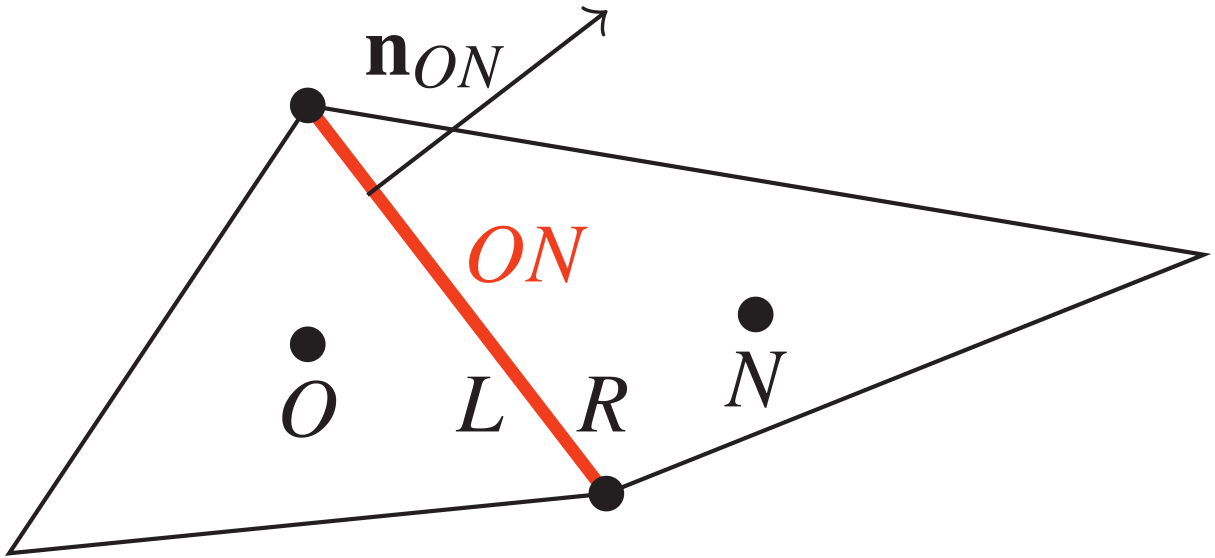
\includegraphics[width=0.4 \linewidth]{Figures/CELL.png}
		\caption[2D computational cell for numerical flux evaluation.]{Computational cell for numerical flux evaluation. \textcolor{red}{ON} represents the interface between the owner cell O and the neighboring cell N, with $n_{ON}$ as the outward normal for O. L and R denote the limit states on either side of the interface, where $L\equiv O$ and $R \equiv O$ in the case of first-order reconstruction.}
		\label{figure:cells}
	\end{figure} 
	
	\noindent Let $\mathbf{\hat{f}}_{ON}$ represent the numerical flux at the interface shared between a given cell and its neighboring cell $N$. The interface area is denoted by $\Delta S_{ON}$, and $\sum_N$ signifies summation over all cell faces.
	\\
	Following the standard AUSM methodology \cite{LIOU_AUSM}, we decompose the Euler fluxes in (\ref{variables})  into two components: one representing convection and the other accounting for pressure, given as:
	
	\begin{equation}
		\mathbf{f}_i = f_i + p_i =
		\begin{Bmatrix}
			\rho u_i \\
			\rho u_i u_j \\
			\rho u_i H
		\end{Bmatrix}
		+
		\begin{Bmatrix}
			0 \\
			p \delta_{ij} \\
			0
		\end{Bmatrix}.
	\end{equation}
	\\
	The corresponding numerical fluxes can be expressed as the sum of a central contribution and a diffusive contribution,both for the convective terms:
	
	\begin{equation}
		\hat{f}_{ON} = \hat{f}^{c}_{ON} + \hat{f}^{D}_{ON}
		\label{convective_central_diffusive_fluxes}
	\end{equation}
	\\
	and the pressure terms:
	
	\begin{equation}
		\hat{p}_{ON} = \hat{p}^{C}_{ON} + \hat{p}^{D}_{ON}.
		\label{diffusive_central_diffusive_fluxes}
	\end{equation}
	\\
	The central part of the convective flux is determined using the following relation \cite{PIROZZOLI20107180}:
	
	\begin{equation}
		\hat{f}^{c}_{ON} = \frac{1}{8} (\rho_0 + \rho_N) (u_{n0} + u_{nN}) (\boldsymbol{\varphi}_0 + \boldsymbol{\varphi}_N),
		\label{PirozzoliFLux}
	\end{equation}
	\\
	where $\boldsymbol{\varphi} = (1, u_i, H)^T$, and the pressure flux is obtained via a standard central interpolation approach:
	
	\begin{equation}
		\hat{p}^{C}_{ON} = \frac{1}{2} (p_0 + p_N).
	\end{equation}
	\\
	Unlike conventional central differencing schemes, the numerical flux in equation (\ref{PirozzoliFLux}) ensures discrete conservation of the total kinetic energy transported by convection, albeit with significant nonlinear stability properties. In fact, this central numerical flux has been observed to maintain stability in fully resolved direct numerical simulations (DNS) on Cartesian grids or slightly distorted meshes \cite{PIROZZOLI20107180,PIROZZOLI20112997}. Nevertheless, when applied to practical computational fluid dynamics problems using unstructured meshes, especially in the presence of shock waves, it becomes necessary to introduce a certain level of numerical diffusion. Consequently, the diffusive fluxes in equation should be selectively activated in regions where resolution deteriorates. To assess local smoothness and determine where numerical diffusion should be applied, a classical shock sensor is employed \cite{DUCROS1999}.
	
	\begin{equation}
		\theta = max\left (\dfrac{-\nabla \cdot \mathbf{u}}{\sqrt{(\nabla \cdot \mathbf{u})^2 + (\nabla \times \mathbf{u})^2 + u_0^2/L_0}}, 0 \right ) \ \in \ [0,1],
	\end{equation}
	\\
	Where $u_0$ and $L_0$ represent appropriate velocity and length scales \cite{Pirozzoli2011}, they are defined such that $ \theta \approx 0 $ in smooth regions and $ \theta \approx 1 $ in the presence of shocks.  
	\\
	For smooth flows (i.e., without shocks), we have observed that numerical stability can be improved with minimal accuracy loss by applying the artificial diffusion term exclusively to the pressure flux, in an amount proportional to $ \theta_{\text{ON}} $. 
	
	\begin{equation}
		\theta_{\text{ON}} = \frac{1}{2} (\theta_O +\theta_N)
	\end{equation}
	\\
	To accurately capture shock waves, it is necessary to also activate the convective diffusive flux whenever $ \theta_{\text{ON}} $ exceeds a specified threshold ($ \theta^* $, set to 0.05 unless stated otherwise). Thus, the diffusive numerical fluxes used in equations (\ref{convective_central_diffusive_fluxes}, \ref{diffusive_central_diffusive_fluxes}) can be concisely expressed as follows:
	
	\begin{equation}
		\hat{f}_{\text{ON}} = (\text{IC}) H (\theta_{\text{ON}} - \theta^*) \tilde{p}_{\text{ON}}^{AUSM}, \quad
		\tilde{p}_D = \text{IP} \theta_{\text{ON}} \tilde{p}_D^{AUSM},
		\label{flags_fluxes}
	\end{equation}
	\\
	$(\text{IC})$ and $(\text{IP})$ are flags that regulate the activation of convective and pressure diffusive fluxes, respectively. $H$ represents the Heaviside step function, while the artificial diffusion fluxes are derived from the AUSM scheme, as outlined in section \ref{AUSMsection}. Recommended values for $(\text{IC})$ and $(\text{IP})$, based on the type of numerical simulation being performed, are provided in table \ref{REF_modes}.  
	
	\begin{table}[h]
		\centering
		\renewcommand{\arraystretch}{1.4} % Adjust row height
		\begin{tabular}{c l l r}
			\hline
			\textbf{Mode} & \textbf{Intent} & \textbf{IC} & \textbf{IP} \\
			\hline
			A & Fully resolved smooth flows & 0 & 0 \\
			B & Unresolved smooth flows & 0 & 1 \\
			C & Shocked flows & 1 & 1 \\
			\hline
		\end{tabular}
				\vspace{3mm}
		\caption{Operational modes of \texttt{rhoEnergyFoam}, with corresponding	suggested values for the flags in equation \ref{flags_fluxes}.}
		\label{REF_modes}
	\end{table}
	\noindent The discretization of viscous fluxes is based on standard second-order approximations for unstructured meshes \cite{hirsch2007numerical} and is implemented using the \texttt{fvc::laplacian()} primitive in OpenFOAM.
	\\The resulting semi-discretized system of ordinary differential equations, say 
	
	\begin{equation}
		\frac{\mathrm{d} \mathbf{u}}{\mathrm{d}t} = R(\mathbf{u}),
	\end{equation}
	\\
	is advanced in time using a low-storage	third-order, three-stage Runge–Kutta algorithm, where the substeps are the following:
	
	\begin{equation}
		\begin{cases}
			\mathbf{u}' = \mathbf{u}^n + \gamma_1 \Delta t\mathbf{R}(\mathbf{u}^n) + \rho_1 \Delta t\mathbf{R}(\mathbf{u}^{n-1})\\
			\mathbf{u}'' = \mathbf{u}' + \gamma_2 \Delta t\mathbf{R}(\mathbf{u}') + \rho_2 \Delta t\mathbf{R}(\mathbf{u}^n)\\
			\mathbf{u}''' = \mathbf{u}'' + \gamma_3 \Delta t\mathbf{R}(\mathbf{u}'') + \rho_3 \Delta t\mathbf{R}(\mathbf{u}')
		\end{cases}	
	\end{equation}
	\\
	where the constants are displayed in table \ref{table:RKconstants}.
	
	\begin{table}[h]
		\centering
		\renewcommand{\arraystretch}{1.6} % Adjust row height
		\begin{tabular}{c c}
			\hline
			\textbf{Constant} & \textbf{Value} \\ 
			\hline 
			$\gamma_1$  & $\frac{8}{15}$ \\
			$\gamma_2$  & $\frac{5}{12}$ \\
			$\gamma_3$  & $\frac{3}{4}$ \\
			$\rho_1$    & $0$ \\
			$\rho_2$    & $-\frac{17}{60}$ \\
			$\rho_3$    & $-\frac{5}{12}$ \\  
			\hline
		\end{tabular}
		\vspace{3mm}
		\caption{Coefficient of the low-storage	third-order, three-stage Runge–Kutta algorithm}
		\label{table:RKconstants}
	\end{table}
	
	\noindent Referring to figure \ref{cells}, the AUSM convective and pressure flux to be
	used in equation (\ref{flags_fluxes}) are given below, based on the AUSM+ -up formulation \citep{LIOU_AUSM+-up}:
	
	\begin{equation}
		\mathbf{\hat{f}}_{ON}^{AUSM} = -\frac{C_{ON}}{2} \left[ \left( \frac{1}{2} \delta m_{ON} - |M_{ON}| \right) \mathbf{\varphi}_L + \left( \frac{1}{2} \delta m_{ON} + |M_{ON}| \right) \mathbf{\varphi}_R \right].
	\end{equation}
	
	\begin{equation}
		\mathbf{\hat{p}}_{ON}^{AUSM} = -\frac{1}{2} \delta \mathbf{p}_{ON},
	\end{equation}
	
	\begin{equation}
		M_{ON} = \frac{M_R + M_L}{2} - \frac{1}{2} \delta m_{ON},
	\end{equation}
	
	\begin{equation}
		\delta m_{ON} = \left[ \Delta \mathcal{M}(M_R) - \Delta \mathcal{M}(M_L) \right] - 2M_p,
	\end{equation}
	
	\begin{equation}
		\Delta \mathcal{M}(M) = \mathcal{M}_{(4)}^+ (M) - \mathcal{M}_{(4)}^- (M),
	\end{equation}
	
	\begin{equation}
		M_p = \frac{k_p}{f_a} \max \left( 1 - \sigma \overline{M}^2, 0 \right) \frac{2(p_R - p_L)}{(\rho_L + \rho_R) c_{ON}^2}.
	\end{equation}
	\\
	The speed of sound at the cell interface is evaluated as 
	
	\begin{equation}
		c_{ON} = \frac{(c_L + c_R)}{2}, \quad \text{and} \quad \overline{M}^2 = \frac{(u_{nL}^2 + u_{nR}^2)}{(2c_{ON}^2)}.
	\end{equation}
	
	\begin{equation}
		M_0^2 = \min(1, \max(\overline{M}^2, M_{\infty}^2)),
	\end{equation}
	
	\begin{equation}
		f_a (M_0) = M_0 (2 - M_0),
	\end{equation}
	\\
	with $ k_p = 0.25 $, $ k_u = 0.75 $, and $ \sigma = 1 $.
	The diffusive-like pressure flux is given by
	
	\begin{equation}
		\delta p_{ON} = \left[ p_R \Delta \mathcal{P}(M_R) - p_L \Delta \mathcal{P}(M_L) \right] - 2M_u.
	\end{equation}
	
	\begin{equation}
		\Delta \mathcal{P}(M) = \mathcal{P}_{(5)}^+ (M) - \mathcal{P}_{(5)}^- (M),
	\end{equation}
	\\
	where
	
	\begin{equation}
		M_u = -\frac{1}{2} k_u \mathcal{P}_{(5)}^+ (M_L) \mathcal{P}_{(5)}^- (M_R) (\rho_L + \rho_R) (f_a c_{ON}) (u_{nR} - u_{nL}).
	\end{equation}
	\\
	The subscript $L, R$ refers to the two sides of the cell interface, which have been reconstructed through the Minmod limiter, also available in the OpenFOAM library. We further define the split Mach numbers $\mathcal{M}_{(m)}$ as $m$-th degree polynomials
	
	\begin{equation}
		\mathcal{M}_{(1)}^{\pm} (M) = \frac{1}{2} (M \pm |M|),
	\end{equation}
	
	\begin{equation}
		\mathcal{M}_{(2)}^{\pm} (M) = \pm \frac{1}{4} (M \pm 1)^2,
	\end{equation}
	
	\begin{equation}
		\mathcal{M}_{(4)}^{\pm} (M) =
		\begin{cases}
			\mathcal{M}_{(1)}^{\pm} (M), & \text{if } |M| \geq 1, \\
			\mathcal{M}_{(2)}^{\pm} (M) (1 \mp 16 \beta \mathcal{M}_{(2)}^{\mp} (M)), & \text{if } |M| < 1.
		\end{cases}
	\end{equation}
	\\
	$P_{(5)}^+$ is also defined in terms of the split Mach numbers, as follows:
	
	\begin{equation}
		P_{(5)}^+ (M) =
		\begin{cases}
			\frac{1}{M} \mathcal{M}_{(1)}^{+} (M), & \text{if } |M| \geq 1, \\
			\mathcal{M}_{(2)}^{+} (M) [(2 \pm M) \mp 16 \alpha M \mathcal{M}_{(2)}^{\mp} (M)], & \text{if } |M| < 1.
		\end{cases}
	\end{equation}
	\\
	Following \citet{LIOU_AUSM+-up}, we set $\alpha = 3/16(-4 + 5 f_a^2)$, $\beta = 1/8$.
	\\
	From its original version, working in OpenFOAM's version v2006, \texttt{rhoEnergyFoam} was then optimized in terms of computational cost and accuracy, and was ported to the ESI OpenFOAM v2412 version. Moreover, the Adaptive Mesh Refinement (AMR) already present in OpenFOAM, has been added as a new feature in \texttt{rhoEnergyFoam} and its results can be seen in section \ref{AMR_cylinder}. 
	
	\subsection{Adaptive Mesh Refinement (AMR)}
	
	Adaptive Mesh Refinement (AMR) is a technique that dynamically refines the computational mesh based on predefined criteria and specific control parameters, such as refinement and unrefinement levels, as well as expansion ratios. In OpenFOAM, AMR is supported by solvers that incorporate dynamic mesh capabilities, with compatibility restricted to hexahedral meshes: itis  available in solvers from the PIMPLE family, and now available also in \texttt{rhoEnergyFoam}. Employing an accurate and stable numerical method is crucial when utilizing AMR. If an unbounded or excessively diffusive method (both in space and time) is used, the refinement strategy may fail to effectively capture the quantity of interest, potentially leading to overshoots and undershoots in the solution. Within OpenFOAM, all dynamic mesh capabilities are controlled in the dictionary \texttt{dynamicMeshDict}, which is located in the \texttt{constant} directory. To appropriately control the time step as the mesh is refined, the recommended approach in OpenFOAM is to enable the \texttt{adjustableTimeStep} option and, maintaining a Courant-Friedrichs-Lewy (CFL) number below $1$, ideally around $0.5$, helps to increase the accuracy of the results. It is important to note that AMR introduces a significant computational overhead, which should be considered when designing simulations. AMR is widely used in various engineering and scientific fields due to its ability to enhance simulation efficiency. In fluid dynamics, it plays a crucial role in turbulent flow simulations, shock capturing, and aeroacoustics by refining areas with high vorticity, shear layers, or boundary layers. In weather and climate modeling, AMR is employed to track the evolution of hurricanes and storms by refining mesh in regions of high vorticity or pressure gradients, thereby improving large-scale atmospheric simulations. It is used in combustion and reactive flow simulations to refine mesh around flame fronts and regions with steep temperature and species concentration gradients. It is also extensively used in structural mechanics and materials science, where it helps to refine regions where cracks propagate in materials and enhances stress analysis by providing higher resolution in high-stress zones. By refining only the necessary regions, AMR allows engineers and scientists to conduct high-fidelity simulations without excessive computational costs, making it a powerful tool for numerical simulations across different disciplines.
	
	\chapter{Test Cases and Results}
	\label{chap:results}
	
	In this chapter, we present a series of test cases that show the capability of rhoEnergyFoam evaluating different test cases where all the three operational modes outlined in table \ref{REF_modes} are analyzed, aiming to evaluate the energy-preserving properties of the proposed solver in comparison to standard OpenFOAM solvers. To assess numerical diffusion, we analyze Euler turbulence and Taylor–Green flow. To assess the capability of AMR, we tested a subsonic turbulent flow past a circular cylinder. To examine the effectiveness of background numerical diffusion in smooth flows, we conduct Unsteady Reynolds-Averaged Navier–Stokes (URANS) and Detached Eddy Simulations (DES) of subsonic turbulent flow past a circular cylinder. To test the accuracy of the solver we simulate the Sod's shock tube. Finally, the shock-capturing capabilities of rhoEnergyFoam are tested using three classical flow cases: inviscid supersonic flow past a forward-facing step, transonic flow past an RAE airfoil, and transonic flow past the ONERA M6 wing.
	
	\section{Decaying Isotropic Turbulence}
	The study of a decaying isotropic turbulence case in the literature serves as a fundamental test for understanding turbulence dynamics in the absence of external forcing or mean flow effects. Isotropic turbulence, characterized by uniform statistical properties in all directions, provides a simplified yet insightful framework to investigate how turbulence evolves over time. Researchers use this case to examine the decay laws of turbulent kinetic energy, the role of vortex structures, and the mechanisms governing the dissipation of energy. It also serves as a benchmark for testing turbulence models, numerical schemes, and theoretical predictions. Since isotropic turbulence eliminates directional biases, it allows for a more general study of turbulence physics that can be applied to a wide range of engineering and geophysical flows. Also, the decay process sheds light on turbulence behavior, understanding mixing, diffusion, and energy cascade processes in both natural and industrial settings.
	In this study, the decay of isotropic turbulence is considered to quantify the energy conservation properties of rhoEnergyFoam, resolving Navier-Stokes equations in the absence of kinematic viscosity ($\nu = 0$). This means that the NS equations becomes the Euler equations as follows
	
	\begin{equation}
		\begin{cases}
			\nabla \cdot u = 0 \\
			\frac{\partial u}{\partial t} + u \cdot \nabla u = - \frac{1}{\rho_0} \nabla p
		\end{cases}
	\end{equation}
	\\
	Numerical simulation was conducted on a structured Cartesian grid consisting of $32^3$ cells (32 cells per side), with uniform spacing and constant timestep, imposing a Courant number (CFL) of 1. Random initial conditions are used with prescribed energy spectrum
	
	\begin{equation}
		E(k) = 16 \sqrt{\frac{2}{\pi}} \frac{u_0^2}{k_0} \left( \frac{k}{k_0} \right )^2 e^{-2(k/k_0)^2}
	\end{equation}
	\\
	where $k_0 = 4$ is the most energetic mode, and $u_0$ is the initial r.m.s. velocity. The Mach number adopted for the simulation was $ Ma= u_0/c_0= 0.01$, where $c_0 = \sqrt{\gamma}$ is the adimensionalized speed of sound. Time is made nondimensional with respect to the eddy turnover time $\tau = 2/k_0 u_0$
	The analysis was carried out by comparing the results obtained with rhoEnergyFoam in three different modes (A, B and C) and rhoCentralFOAM. In addition, the case was also evaluated using the dnsFOAM solver for a more in-depth comparison.
	
	\begin{figure}[h]
		\centering
		\hspace{20mm}
		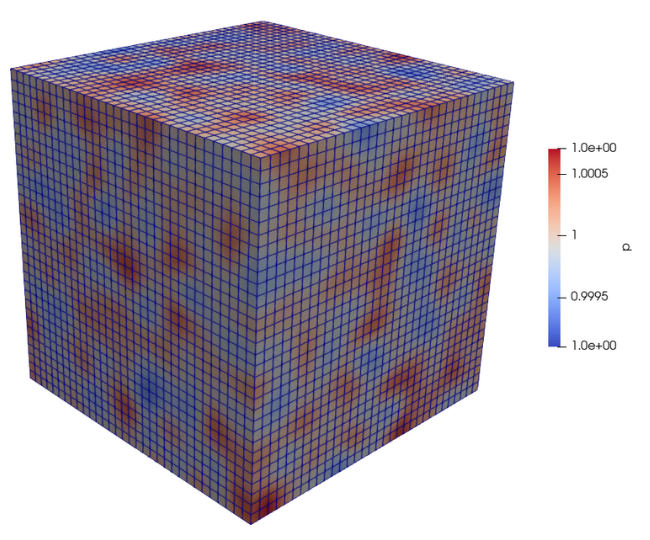
\includegraphics[width=0.6\linewidth]{Figures/DIT}
		\caption{Structured mesh for numerical simulation of decaying isotropic turbulence.}
		\label{DIT_mesh}
	\end{figure}
	
	\begin{figure}[h]
		\centering
		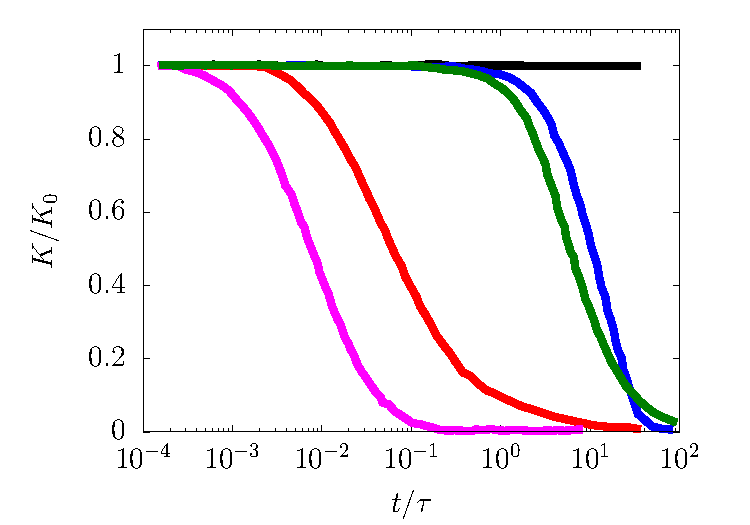
\includegraphics[width=0.7\linewidth]{Figures/TKE_DIT}
		\caption[Turbulence kinetic energy for the decaying isotropic turbulence case]{Decaying isotropic turbulence: time evolution of turbulence kinetic $K$ energy for rhoEnergyFoam in Mode A (black line), Mode B (blue line), Mode C with $\theta^* = 0$ (red line), for dnsFOAM (green line), and rhoCentralFoam (magenta line). $\tau$ is the eddy turnover time.}
		\label{DIT}
	\end{figure} 
	
	\begin{equation}
		\text{CFL} = \max \left( \frac{(u_0 + c_0) \Delta t}{\Delta x} \right).
	\end{equation}
	\\
	The evolution of turbulence kinetic energy defined as:
	
	\begin{equation}
		K = \frac{1}{2} \sum_i  (u_{k} u_{k})_i V_i,
	\end{equation}
	\\
	where $u_k$ represents the velocity of the cell $i$, $V_i$ is the volume of cell, can be seen in figure \ref{DIT}.
	\begin{table}[h]
		\centering
		\begin{tabular}{cc}
			\toprule
			rhoEnergyFoam - mode A &  \textcolor{black}{\rule{0.05\linewidth}{0.75mm}} \\
			rhoEnergyFoam - mode B &  \textcolor{blue}{\rule{0.05\linewidth}{0.75mm}} \\
			rhoEnergyFoam - mode C &  \textcolor{red}{\rule{0.05\linewidth}{0.75mm}} \\
			rhoCentralFoam	  	   &  \textcolor{magenta}{\rule{0.05\linewidth}{0.75mm}} \\
			dnsFoam			       &  \textcolor{green}{\rule{0.05\linewidth}{0.75mm}} \\
			\bottomrule
		\end{tabular}
	\end{table}
	From an aerospace engineering perspective, accurately capturing turbulent kinetic energy dynamics is crucial, particularly in high-speed aerodynamic flows where shock-boundary layer interactions and numerical diffusion can significantly impact predictive accuracy. The numerical study is conducted with convective diffusive fluxes initially deactivated (mode A) to assess the upper bound of numerical diffusion in shock-capturing simulations.
	\\
	To benchmark the solvers, results from \texttt{rhoCentralFoam} and the incompressible Direct Numerical Simulation (DNS) solver \texttt{dnsFoam} from OpenFOAM are also presented. The findings indicate that neither of the standard OpenFOAM solvers can preserve total kinetic energy effectively due to inherent numerical diffusion, which is particularly noticeable in \texttt{rhoCentralFoam}. The results given from \texttt{rhoEnergyFoam} show that it conserves total kinetic energy under Mode A operation, aligning with theoretical expectations for energy-preserving schemes.
	\\
	When the pressure diffusion term is introduced (Mode B), a degree of numerical diffusion is observed, albeit lower than in \texttt{dnsFoam}. Most kinetic energy is dissipated at the characteristic eddy turn-over time scale. In Mode C, where $\theta^* = 0$, numerical diffusion is exacerbated but remains less pronounced than in \texttt{rhoCentralFoam}. 
	
	\section{Taylor-Green Vortex}
	The Taylor–Green vortex solution is a classical case used for testing and validating spatial and temporal accuracy of CFD solvers. In fact, the Taylor-Green vortex illustrates the fundamental process of decaying production of small vortices, known as eddies.The energy-preserving properties of \texttt{rhoEnergyFoam} are herein tested checking the time reversibility of this test case. Tests were conducted on two types of meshes: a structured one (figure (\ref{TGV_mesh}.a)) with $32'768$ cubic cells and a unstructured one (figure (\ref{TGV_mesh}.b)) with $85'056$ prisms. Both of them are a $(2\pi)^3$ triply-periodic box generated with Gmsh (an open source finite-element mesh generator). The unstructured mesh was made extruding the triangular elements of the frontal face along the third dimension. This setting guarantees exact geometrical correspondence of the elements on opposite faces of the computational box, hence periodicity can be exploited in all space directions.
	
	\begin{figure}[h]
		\centering
		(a)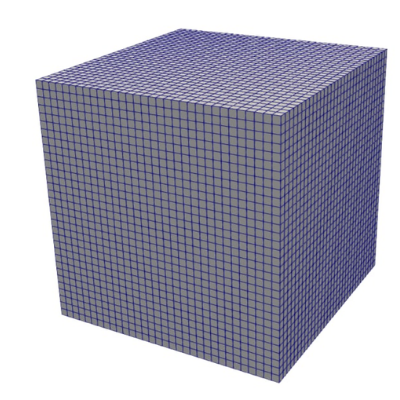
\includegraphics[width=0.4\linewidth]{Figures/TGV_mesh_structured}
		(b)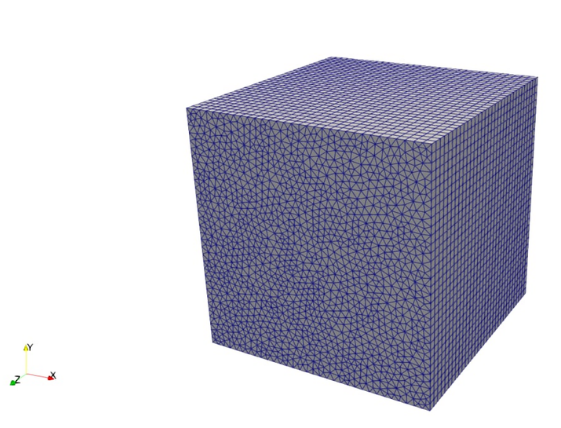
\includegraphics[width=0.4\linewidth]{Figures/TGV_mesh_unstructured}\\
		\caption{Structured mesh (a) and unstructured mesh (b)for numerical simulation of Taylor–Green flow.}
		\label{TGV_mesh}
	\end{figure} 
	
	\noindent To verify the conservation of Turbulent Kinetic Energy (TKE), a time reversal test was performed in the middle of the simulation to ensure that the solution returned to the values of the initial conditions. 
	The solution was initialized as follows:
	
	\begin{equation}
		\begin{cases}
			u = u_0 sin(k_0 x)cos(k_0 y)cos(k_0 z)\\
			v = -v_0 cos(k_0 x)sin(k_0 y)cos(k_0 z)\\
			w = 0
		\end{cases}
	\end{equation}
	\\
	where the density is constant $\rho = \rho_0$, $u_0 = Ma \ c_0$ is the reference velocity with $Ma = 0.01$ and $c_0$ is the reference speed of sound, $P_0$ is the reference pressure and $T_0$ is the reference temperature. The pressure equation used to initialize the case was the following:
	
	\begin{equation}
		p = p_0 + \frac{u_0^2}{16}[cos(2k_0 x)+sin(2k_0 y)][2+ cos(2k_0 z)]		
	\end{equation}
	\\
	where $k_0 = 1$ is the initial wave number. 
	The initial conditions on the velocity field represented with the Q-criterion are show in figure (\ref{TGV_Qcriterion})
	
	\begin{figure}[h]
		\centering
		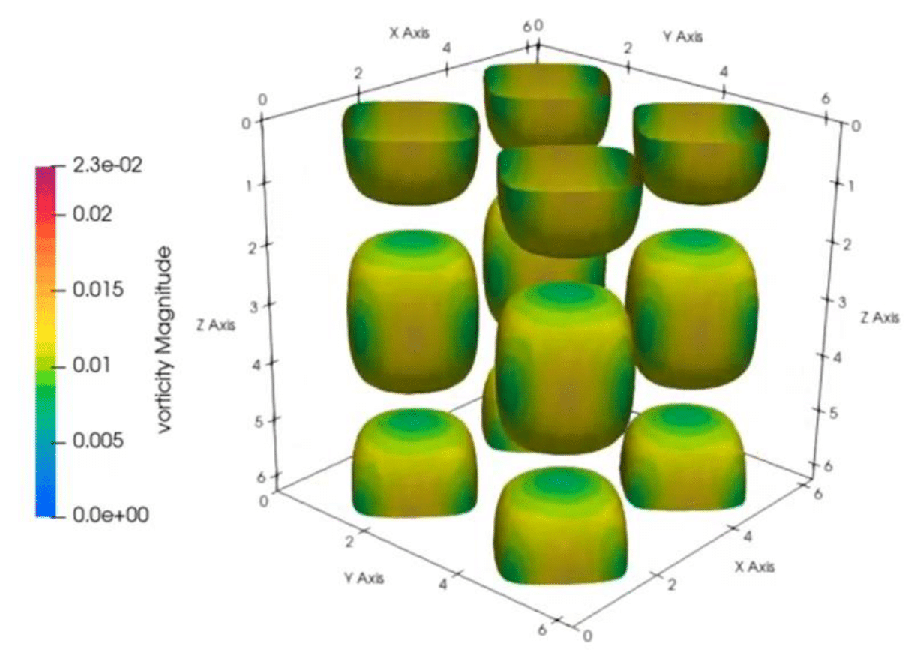
\includegraphics[width=0.7\linewidth]{Figures/TGV_Qcriterion}
		\caption{Vorticity field visualized using the Q-criterion for the Taylor-Green Vortex.}
		\label{TGV_Qcriterion}
	\end{figure}
	The solution is evolved over time until $t u_0 k_0 = 8$, where all velocity vectors are reversed, and then continued further until $t u_0 k_0 = 16$. According to the mathematical principles governing the Euler equations, the initial conditions are expected to be precisely recovered.
	\\
	Herein, we introduce a new physical variable called Enstrophy, defined as
	\begin{equation}
		\Omega = \frac{1}{2} \sum_i (\omega_k \omega_k)_i V_i.
	\end{equation}
	\\
	where $\omega = \nabla \times u$ represents the vorticity of the cell $i$ and $V_i$ is the volume of cell. Enstrophy is a measure of the intensity of vorticity in a moving fluid. In turbulence theory it provides insights into the distribution and dissipation of rotational motion within a flow. In inviscid flows, enstrophy can be conserved, whereas in viscous flows, it tends to dissipate over time due to the effects of viscosity.	The evolution in time of the turbulent kinetic energy and of the enstrophy can be seen in figure (\ref{TKE_ENS_TGV}). As illustrated in panel (a), the kinetic energy obtained from the simulation on the structured mesh using \texttt{rhoEnergyFoam} in both mode A and mode B remains conserved and constant, as indicated by the black solid line and the blue dotted line. In contrast, \texttt{rhoCentralFoam} exhibits a rapid dissipation of kinetic energy over a very short timescale, with curves that are nearly imperceptible in the adopted representation. Meanwhile, \texttt{dnsFoam} demonstrates a gradual decay of kinetic energy. In panel (b), which corresponds to the unstructured mesh, the total kinetic energy obtained using \texttt{dnsFoam} exhibits a continuous decay, whereas \texttt{rhoCentralFoam} continues to show rapid dissipation of kinetic energy. Conversely, \texttt{rhoEnergyFoam} effectively preserves kinetic energy in mode A, while mode B experiences some degree of numerical diffusion.
	In the Cartesian grid (panel c), the total enstrophy experiences a significant increase up to the point of time reversal, after which it symmetrically decreases. However, with \texttt{dnsFoam}, the initial conditions are not perfectly restored, as the maximum vorticity at the conclusion of the simulation exceeds the expected value. This discrepancy arises from the randomization of the flow at the end of the direct phase, which is not entirely recovered in simulations influenced by numerical diffusion. On the unstructured grid (panel d), a similar trend is observed. Indeed, \texttt{rhoEnergyFoam} in mode A (black line) retains initial conditions, while \texttt{rhoEnergyFoam} in mode B shows a lower peak due to errors associated with mesh distortion and to the introduction of diffusion. In both cases, \texttt{dnsFoam} and \texttt{rhoCentralFoam} are not able to show good results.
	
	\begin{figure}[h]
		\centering
		(a)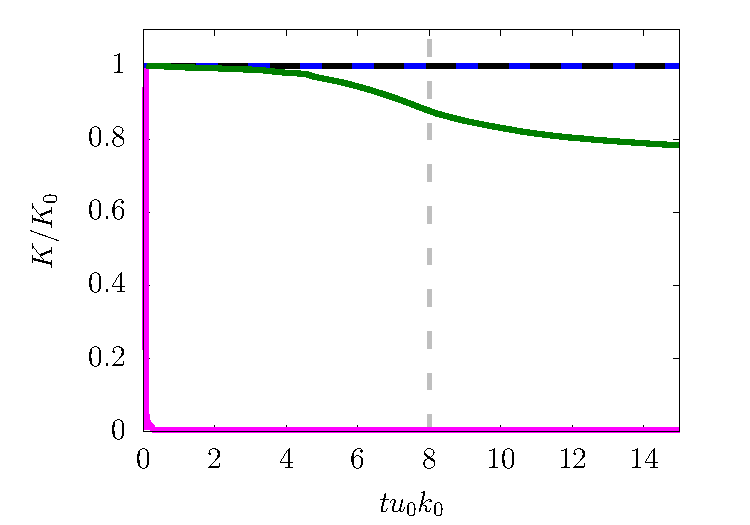
\includegraphics[width=0.45\linewidth]{Figures/TKE_TGV_structured}
		(b)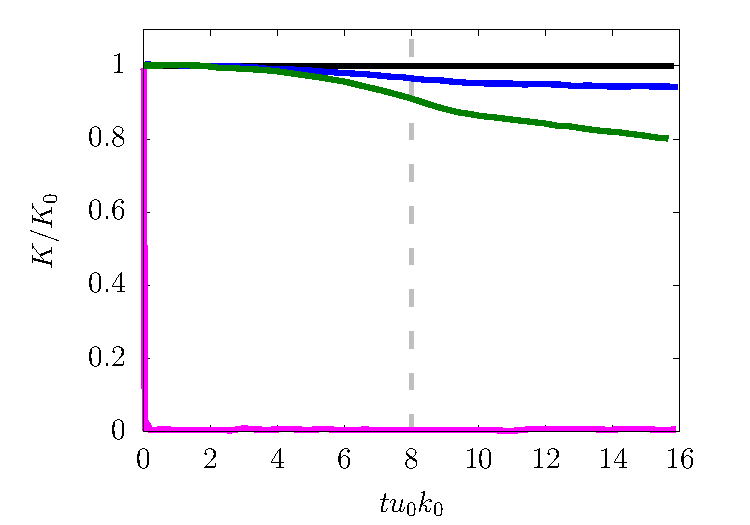
\includegraphics[width=0.45\linewidth]{Figures/TKE_TGV_unstructured}\\
		(c)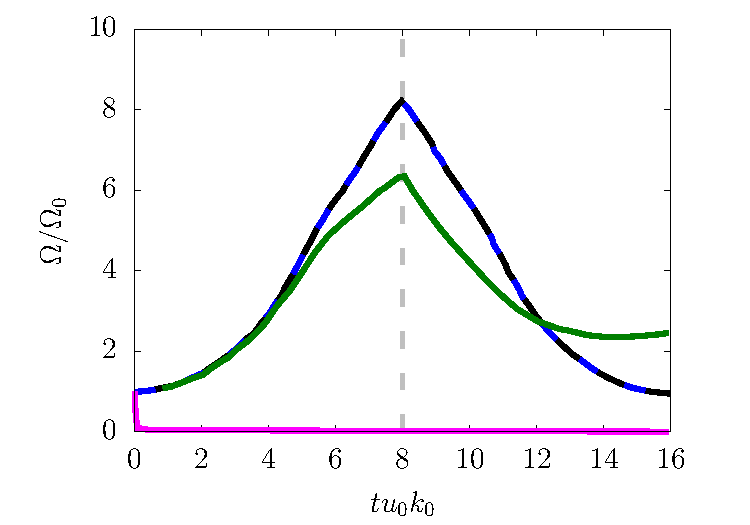
\includegraphics[width=0.45\linewidth]{Figures/ENS_TGV_structured}
		(d)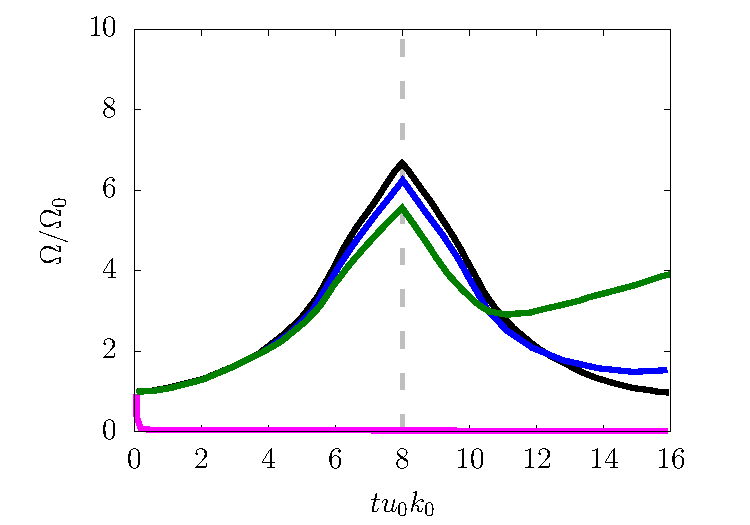
\includegraphics[width=0.45\linewidth]{Figures/ENS_TGV_unstructured}\\
		\caption[Turbulence kinetic energy and enstrophy plots for the Taylor Green Vortex case.]{Taylor Green Vortex: time evolution of total kinetic energy (a-b), and enstrophy (c-d) for Taylor–Green flow at $Ma = 0.01$ on Cartesian mesh (a–c) and on unstructured mesh (b–d). Data are shown for rhoEnergyFoam in Mode A (black line), Mode B (blue dotted line), for dnsFOAM (green line) and rhoCentralFoam (magenta line).}
		\label{TKE_ENS_TGV}
	\end{figure}  
	
	\section{Smooth flow past cylinder with AMR}
	\label{AMR_cylinder}
	
	The subsonic flow around a circular cylinder is here analyzed to check whether the upgrade of \texttt{rhoEnergyFoam} with the Adaptive Mesh Refinement (AMR) schemes (already present within OpenFOAM) works as expected. The simulation is performed on a 2D  circular cylinder at Mach $M_\infty = u_0/c_0 = 0.1$, where $c_0 = \sqrt{\gamma R T_0}$ is the adimensionalized speed of sound, $R = 1$ is the adimensionalized Gas constant and $T_0 =1$ is the non-dimensional initial temperature. $u_0$ is the initial velocity field obtained with the previous equation, knowing the value of $c_0$ and of $M_\infty$. The simulation is set using non-dimensional quantities such as the Reynolds number $Re_\infty = 100$, which is defined as 
	
	\begin{equation}
		Re = \frac{\rho_\infty u_0 D}{\mu_\infty}
	\end{equation}
	\\
	where $\rho_\infty$ is the density of the fluid, $D$ is the cylinder diameter, and $\mu_\infty$ is the dynamic viscosity. Also, the boundary of the domain used are $L_x = 14D$, $L_z = 8D$. 
	The variables used are shown in table \ref{tab:cylinder_2d}.
	
	\begin{table}[h]
		\centering
		\begin{tabular}{lcc}
			\hline
			Variable & Value \\
			\hline
			$M_{\infty}$ & 0.1 \\
			$Re_{D}$ & $100$ \\
			$\rho_{\infty}$ & 1 \\
			$u_{\infty}$ & 0.118321 \\
			$c_{\infty}$ & 1.18321 \\
			$\mu_{\infty}$ & $1.18321 \times 10^{-4}$ \\
			$D$ & 0.1 \\
			\hline
		\end{tabular}
		\vspace{3mm}
		\caption{Initial conditions for turbulent flow around 
			circular cylinder.}
		\label{tab:cylinder_2d}
	\end{table}
	
	\noindent The carthesian mesh, having $14'196$ cells, is generated through the \texttt{blockMesh} utility, then it has been refined through the \texttt{snappyHexMesh} utility, as shown in figure (\ref{Cylinder_u1}). 
	
	\begin{figure}[h]
		\centering
		{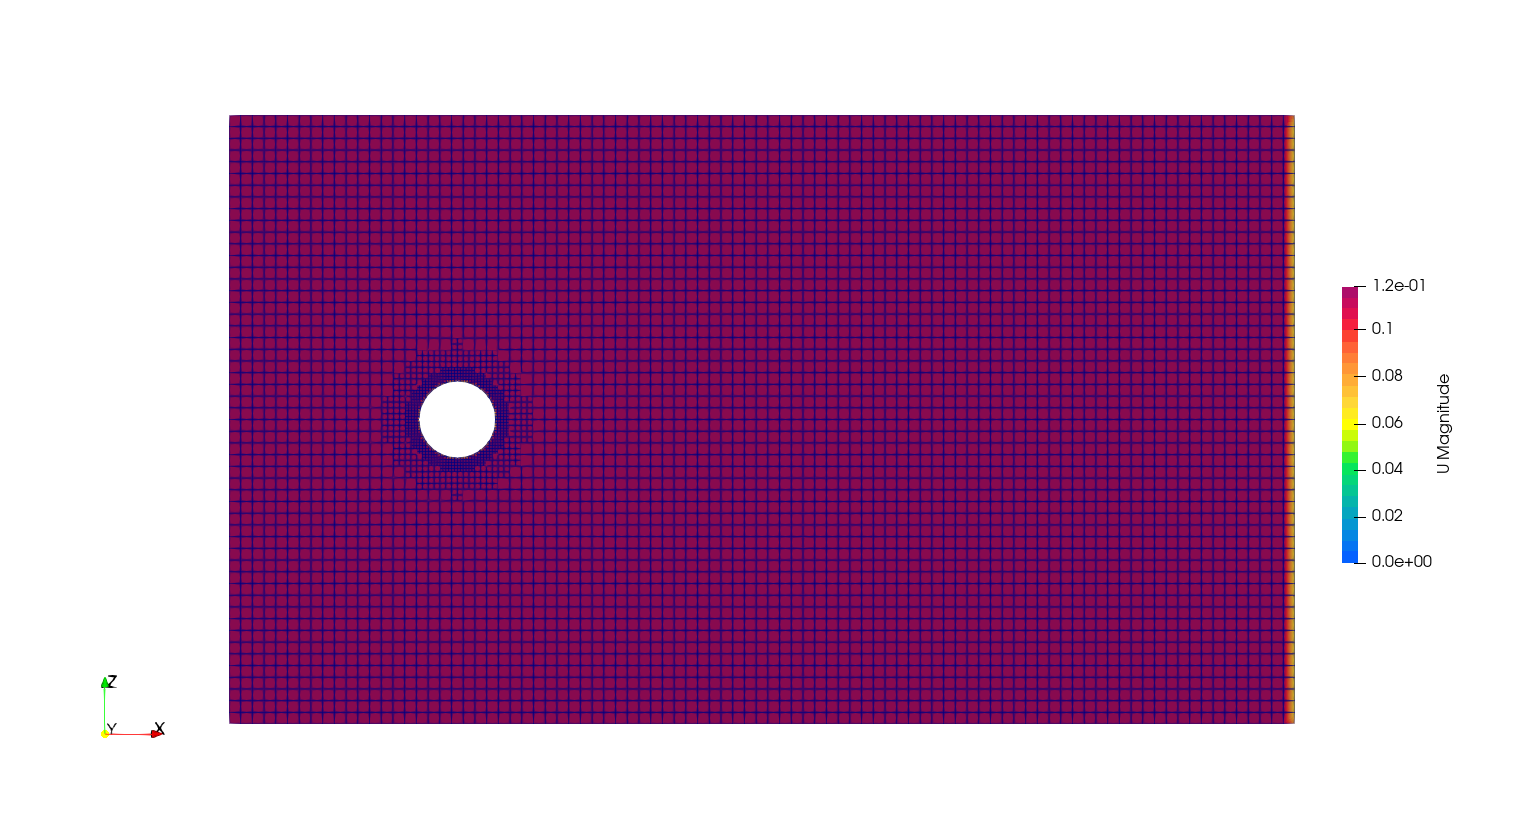
\includegraphics[width=0.58\linewidth]{Figures/Cylinder_u1}} 
		\caption[Smooth flow past cylinder with AMR: initial velocity field.]{Smooth flow past cylinder with AMR: initial velocity field, with the mesh refinement only around the cylinder.}
		\label{Cylinder_u1}
	\end{figure}
	
	\noindent In figure (\ref{Cylinder_u1}), the initial velocity field is displayed, showing a uniform inflow condition and uniform velocity distribution around the cylinder. 

	\begin{figure}[h]
		\centering
		{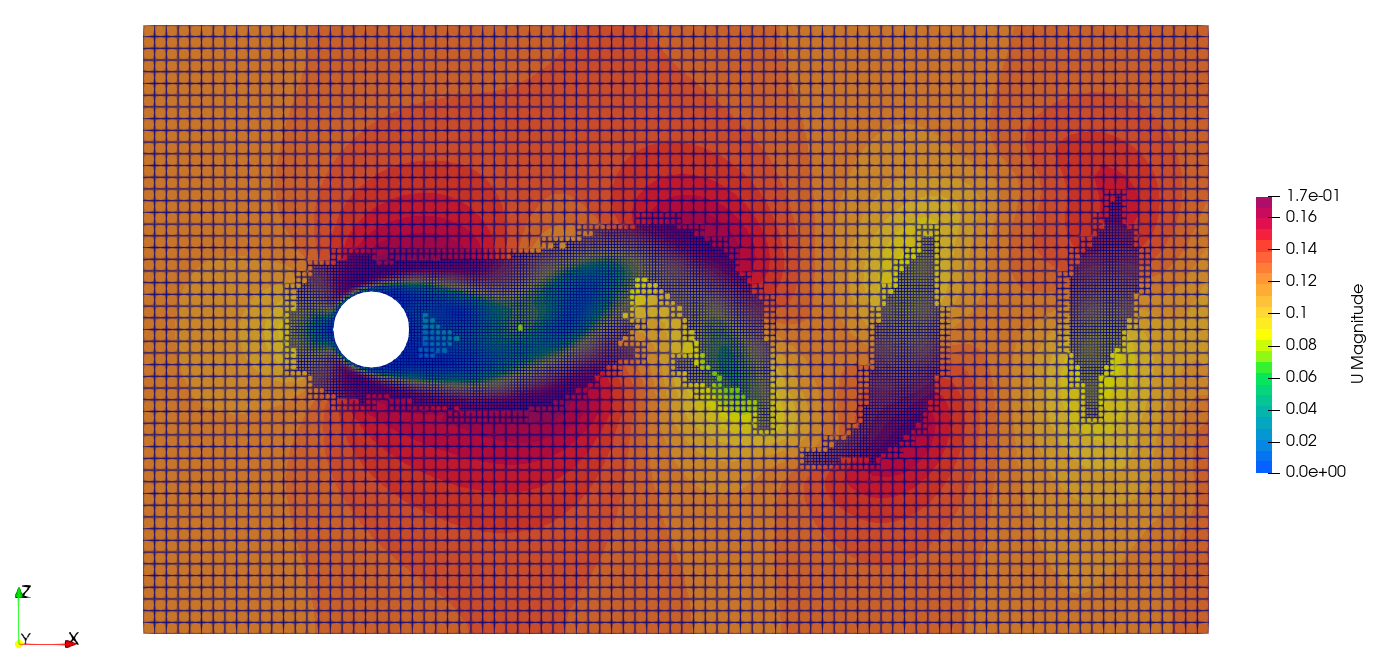
\includegraphics[width=0.58\linewidth]{Figures/Cylinder_u2}}  
		\caption[Smooth flow past cylinder with AMR: vortex shedding.]{Smooth flow past cylinder with AMR: velocity field which shows the vortex shedding and the Kármán vortex street possible through the refinement of the mesh in the necessary zones.}
		\label{Cylinder_u2}
	\end{figure}
	
	\noindent In figure (\ref{Cylinder_u2}), the velocity field illustrates the onset of vortex shedding, characterized by alternating vortices in the wake of the cylinder. This phenomenon is known as vortex shedding an its pattern is typical for flows in the moderate Reynolds number regime, where the wake becomes unsteady and leads to the formation of the well-known Von Kármán vortex street.
	
	\begin{figure}[h]
		\centering
		{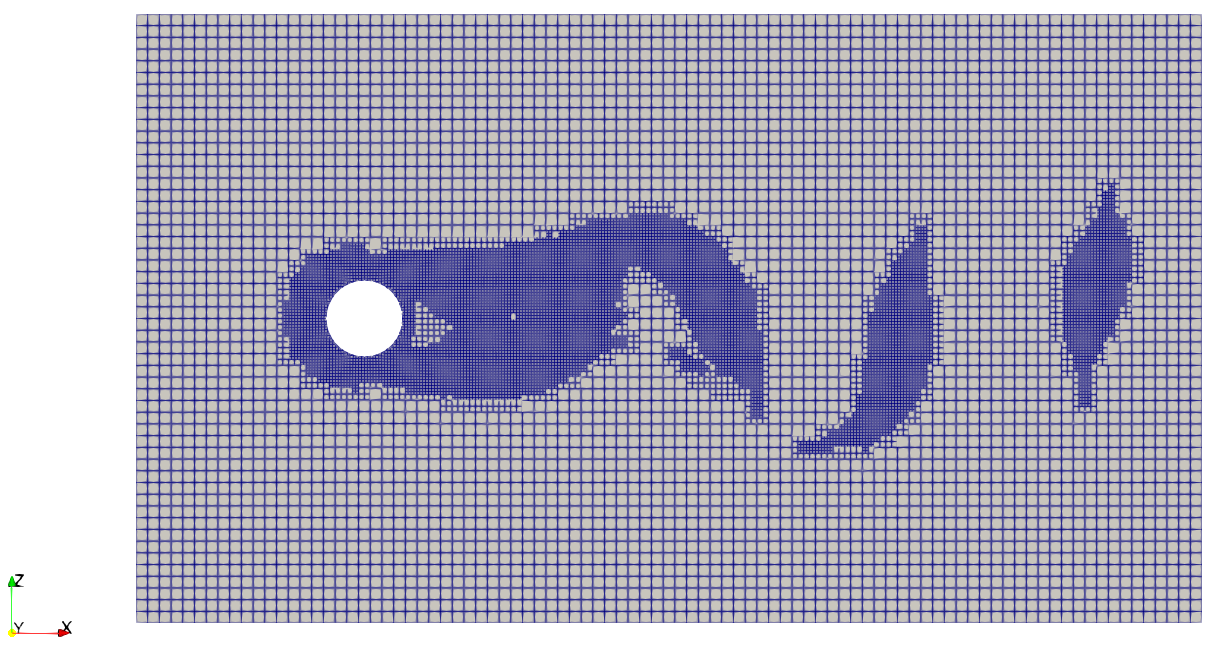
\includegraphics[width=0.51\linewidth]{Figures/Cylinder_mesh_AMR}}
		\caption{Cylinder mesh AMR.}
		\label{Cylinder_mesh_AMR}
	\end{figure}
	
	\noindent Overall, the results highlight the transition from an initial steady-state condition to an unsteady wake due to flow separation and periodic vortex shedding.
	

	\section{URANS and DES of a flow \\ past circular cylinder}
	The turbulent flow around a circular cylinder has been numerically investigated using \textit{rhoEnergyFoam} in mode B, employing both URANS (Unsteady Reynolds-Averaged Navier-Stokes) and DES (Detached Eddy Simulation). The study is based on the classic Spalart-Allmaras turbulence model and its DES extension. The free-stream Mach number is given by $M_0 = u_0/c_0 = 0.1$,	where $u_0$ and $c_0$ are the free-stream velocity and the speed of sound. The Reynolds number, based on the cylinder diameter, is defined as $Re_D = (\rho_0 u_0 D)/\mu_w$, where $\rho_0$ represents the free-stream density and $\mu_w$ the wall viscosity. For the URANS simulation, an O-type mesh is utilized, consisting of $ N_r \times N_\theta = 256 \times 256 $ cells, with a hyperbolic tangent stretching towards the wall in a computational domain of $ L_r \times L_z = 20D \times 2D $, as shown in figure \ref{Cylinder_mesh}. For the DES simulation, an also an O-type mesh is utilized, consisting of $ N_r \times N_\theta \times N_z = 256 \times 256 \times 48 $ cells. Here as well, a hyperbolic tangent stretching towards the wall was used, within the same domain as written above. The grid is refined near the cylinder, with the first grid point located at $ y_+ \approx 150 - 200 $, necessitating the use of wall functions for proper wall treatment. Specifically, Spalding’s equilibrium wall law \citep{spalding1961single} is employed. 
	
	\begin{figure}[h]
		\centering
		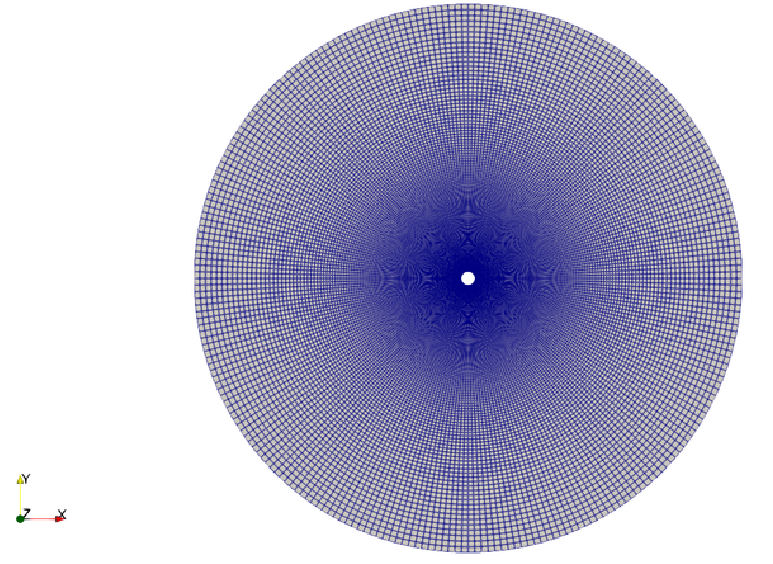
\includegraphics[width=0.7 \linewidth]{Figures/Cylinder_mesh}
		\caption[Mesh for the URANS and DES simulation of the cylinder]{Mesh for the URANS ($ N_r \times N_\theta \times N_z = 256 \times 256$) and DES ($ N_r \times N_\theta \times N_z = 256 \times 256 \times 48 $) simulation of the flow over a circular cylinder.}
		\label{Cylinder_mesh}
	\end{figure} 
	
	\begin{figure}[h]
		\centering
		(a){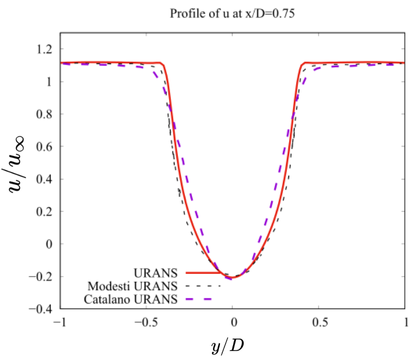
\includegraphics[width=0.4\textwidth]{Figures/Cylinder_u_075}}
		(b){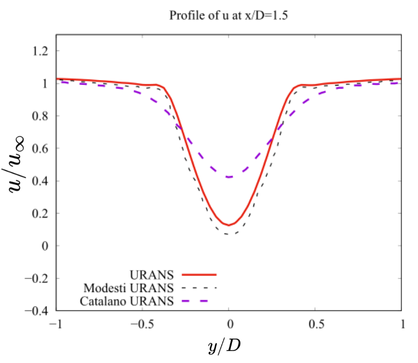
\includegraphics[width=0.4\textwidth]{Figures/Cylinder_u_150}}\\
		(c){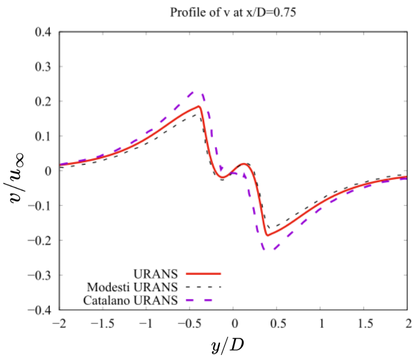
\includegraphics[width=0.4\textwidth]{Figures/Cylinder_v_075}}
		(d){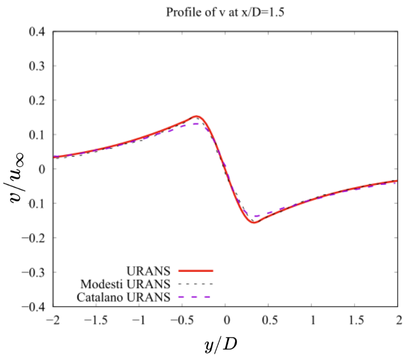
\includegraphics[width=0.4\textwidth]{Figures/Cylinder_v_150}}
		\caption[Velocity profiles of a URANS for a flow around cylinder]{Numerical simulation of flow around circular cylinder: mean velocity profiles at $x/D = 0.75$ (panels a-c) e $x/D = 1.5$ (panels b-d) for URANS with \texttt{rhoEnergyFoam} (red line), Modesti's URANS (black dotted line) Catalano's URANS (purple dotted line).}
		\label{Cylinder}
	\end{figure}
	
	\noindent Isothermal no-slip boundary conditions are imposed at the wall, while \texttt{fixedValue} and/or \texttt{zeroGradient} boundary conditions are applied to all variables at the inlet and outlet, respectively. The turbulent viscosity is set to $\mu_{t0} = 3\mu_w$. The simulation has been performed in parallel, dividing the computational domain within 48 processors, in an HPC architecture. Numerical results are compared against previous simulations and experimental data. In figure \ref{Cylinder} we present mean velocity profiles in the cylinder wake, whose results are of good acceptance with previous studies, with the only discrepancy that there is a longer wake in URANS compared to the reference numerical simulations by Catalano \cite{Catalano}. This deviation is likely caused by an inaccurate prediction of the separation point due to the approximate wall treatment. A key difference observed in URANS is the absence of significant vortex shedding, likely due to the use of wall functions. In contrast, vortex shedding is captured in the DES simulation, as shown in figure~(\ref{Des_Cylinder}), with global flow parameters in reasonable agreement with reference sources. Further analysis of the wall pressure coefficient for the URANS and DES is presented in figures~(\ref{Cp_Cylinder_URANS}, \ref{Cp_Cylinder_DES}). The overall comparison is satisfactory.
		
	\begin{figure}[h]
		\begin{center}
			\hspace{5mm}
			{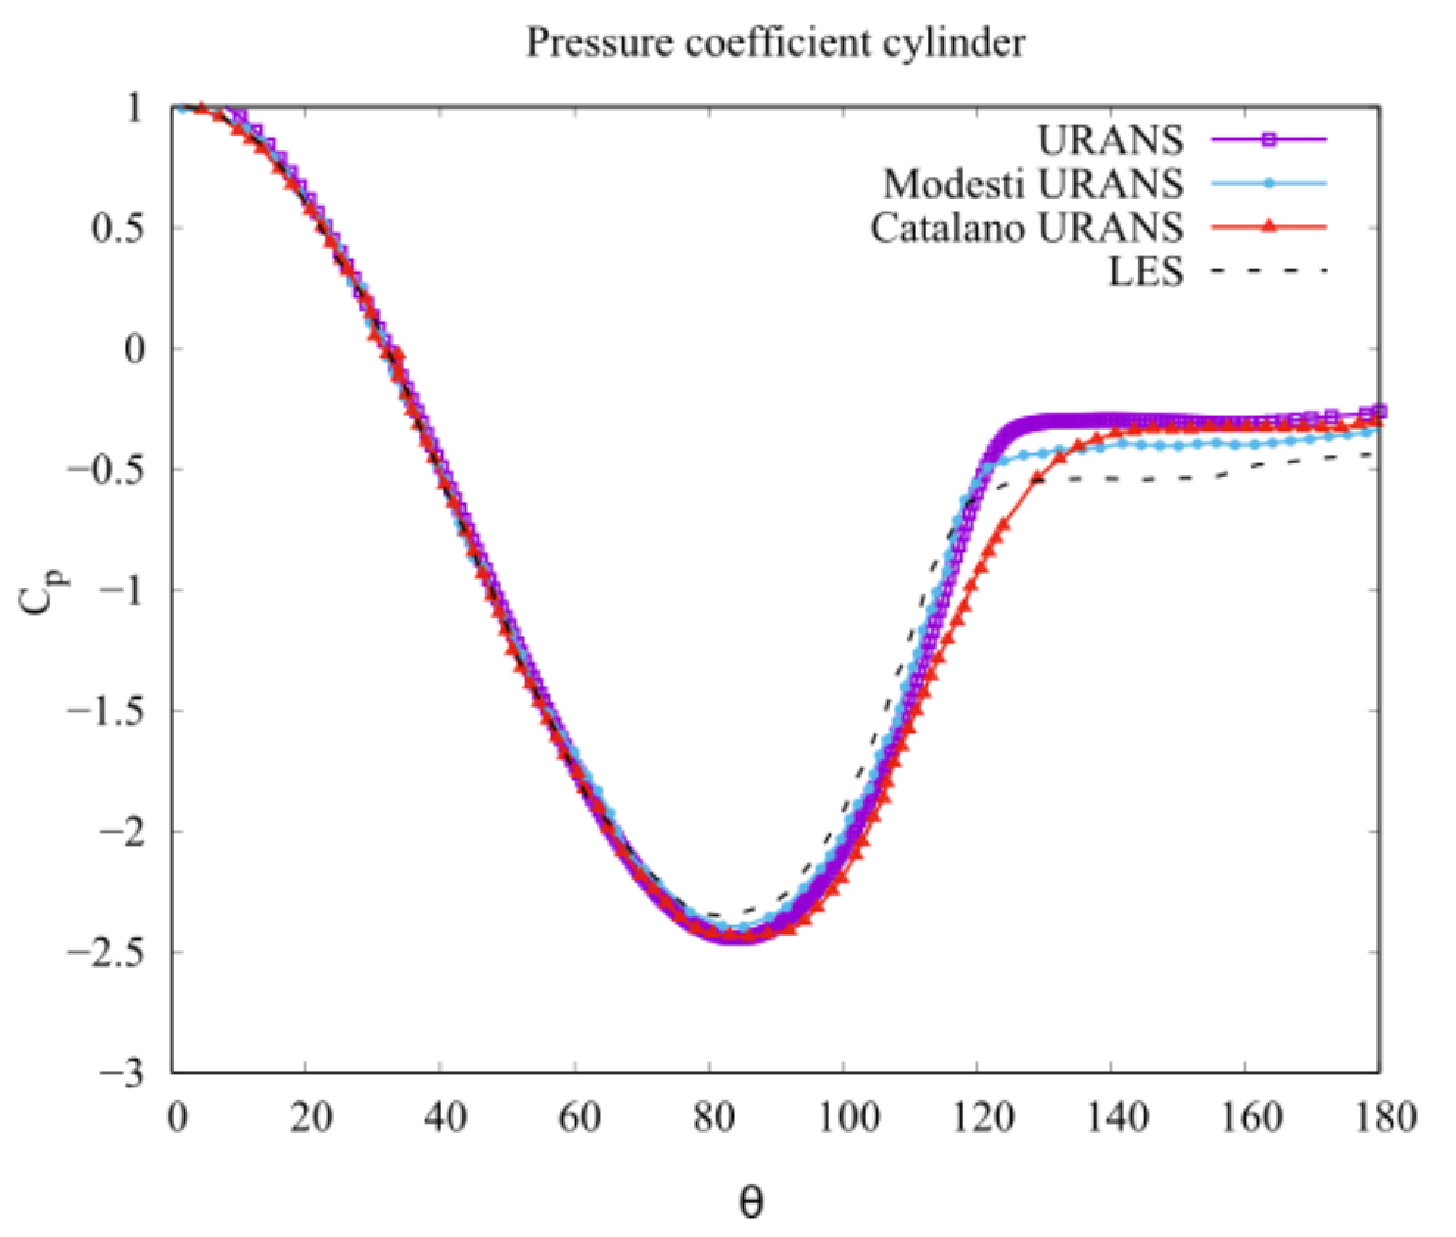
\includegraphics[width=0.46\linewidth]{Figures/pressure_coeff_cylinder}}  
			\caption[Pressure coefficients for the URANS of the 2D cylinder]{Numerical simulation of flow around a 2D circular cylinder: wall pressure coefficient obtained from rhoEnergyFoam in Mode B with URANS (purple line) Modesti's URANS (light blue line) and Catalano's URANS and LES (black dotted line).}
			\label{Cp_Cylinder_URANS}
		\end{center}
	\end{figure}
	
	\begin{figure}[h]
		\begin{center}
			{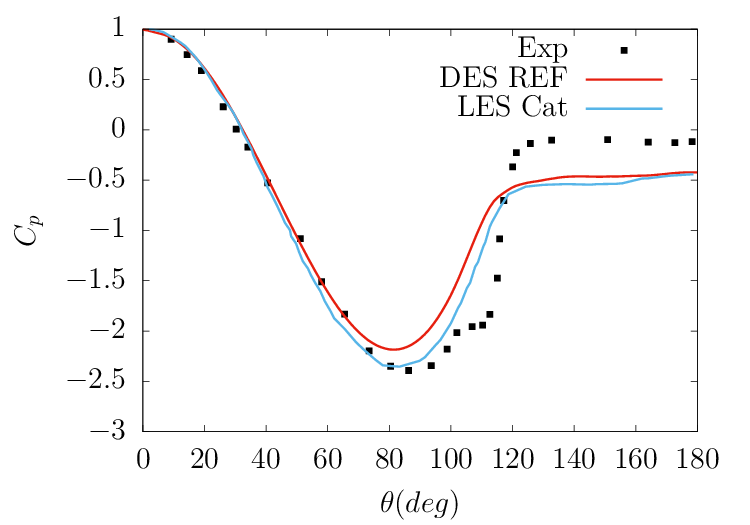
\includegraphics[width=0.56\linewidth]{Figures/pressure_coefficient_DES}}  
			\caption[Pressure coefficients for the DES of the 3D cylinder]{Numerical simulation of flow around a 3D circular cylinder: wall pressure coefficient obtained from rhoEnergyFoam in Mode B with DES (red line) and Catalano's DES (light blue line).}
			\label{Cp_Cylinder_DES}
		\end{center}
	\end{figure}
	
	\begin{figure}[t]
		\begin{center}
			{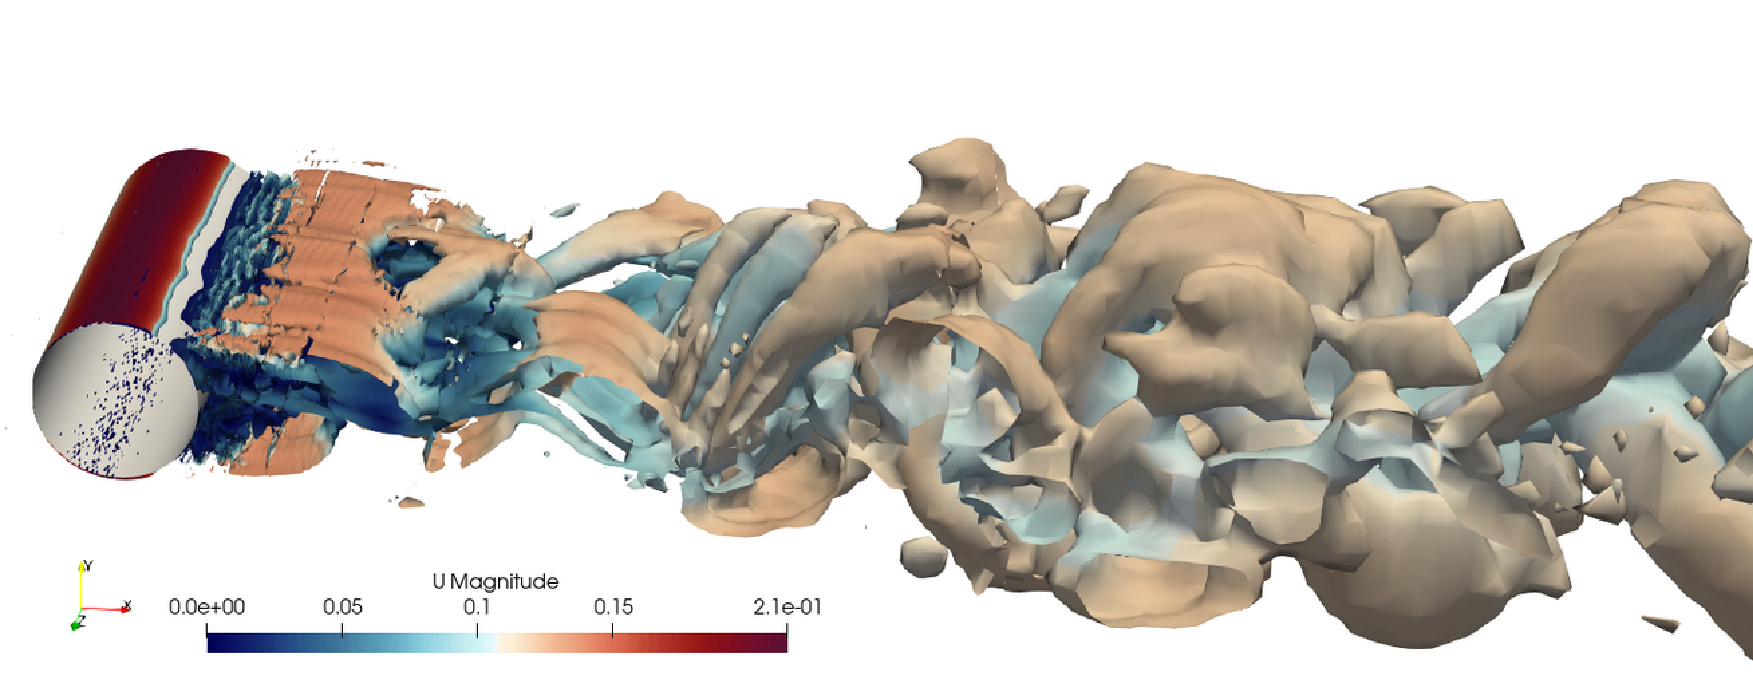
\includegraphics[width=1\linewidth]{Figures/Des_cylinder}}
			\caption[Velocity representation through Q-criterion of a DES of the circular cylinder]{DES of a flow over a 3D circular cylinder: velocity filed plotted with Q-criterion $Q = \dfrac{1}{2} [(\nabla \cdot u)^2 - \nabla u : \nabla u^T]$.}
			\label{Des_Cylinder}
		\end{center}
	\end{figure}
	\newpage
	\section{Sod's shock tube}
	In this case, we simulate the Sod's shock tube problem, named after Gary A. Sod. This is a common test for the accuracy of computational fluid codes, like Riemann solvers, and was heavily investigated by \citet{Sod19781} in 1978. It consists of a pipe with either a circular or rectangular cross-section, filled with gas. The pipe is divided into two regions by a diaphragm positioned at its midpoint, as illustrated in figure (\ref{Sod_geometry}). 
		
	\begin{figure}[h]
		\centering
		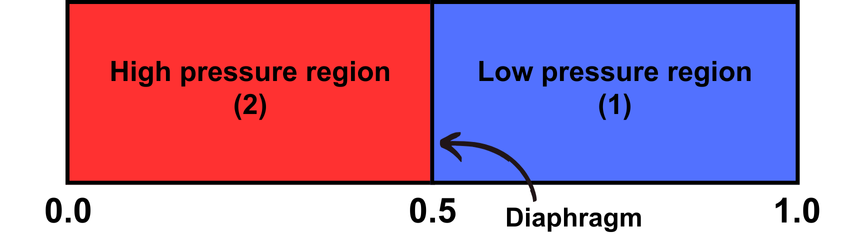
\includegraphics[width=0.8 \linewidth]{Figures/SOD_TUBE_GEOMETRY}
		\caption{Sod shock tube at $t = 0$. On the left-hand side region with high density, pressure and temperature}
		\label{Sod_geometry}
	\end{figure} 
	
	\noindent In numerical simulations, this diaphragm is represented as a discontinuity in the initial fluid conditions, including density, pressure, and temperature, across the interface. This is an extremely severe case used to test the accuracy and stability of CFD solvers. The initial conditions for this problem are straightforward, consisting of a contact discontinuity that separates gas regions with different pressure and density, while the velocity remains zero throughout the domain. In the standard configuration, the left side of the diaphragm has a density and pressure of $1$, whereas the right side has a density of $0.125$ and a pressure of $0.1$. The specific heat ratio is set to $1.4$.\\
	These initial conditions can be expressed mathematically as follows. 
	
	\begin{equation}
		\begin{bmatrix}
			\rho_2\\
			P_2\\
			u_2
		\end{bmatrix}
		=
		\begin{bmatrix}
			1.0\\
			1.0\\
			0.0
		\end{bmatrix},
		\quad
		\begin{bmatrix}
			\rho_1\\
			P_1\\
			u_1
		\end{bmatrix}
		=
		\begin{bmatrix}
			0.125\\
			0.1\\
			0.0
		\end{bmatrix}
	\end{equation}
	\\
	where $\rho$ is density, $P$ is pressure and $u$ is velocity. Index $(2)$ and $(1)$ refer to left and right-hand side conditions on the side of the diaphragm, respectively. The equations to be solved are the Euler equations, the air is modeled as an ideal gas and, in this case, \texttt{rhoEnergyFoam}0 is used in Mode C, where full AUSM \ref{AUSMsection} diffusion is activated near discontinuities to ensure stability and accuracy. The results
	are for similar runtime parameters (CFL, time step), accuracy and mesh. 

	\begin{figure}
		\centering
		(a)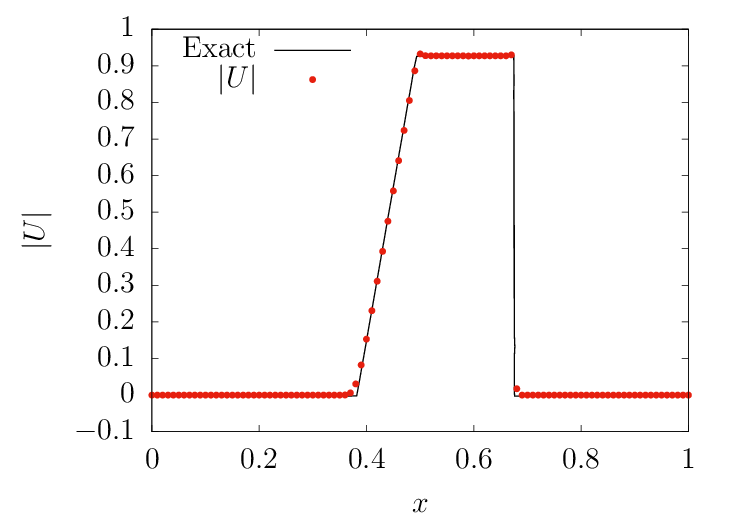
\includegraphics[width=0.45\linewidth]{Figures/Sod_umag_ref}
		(b)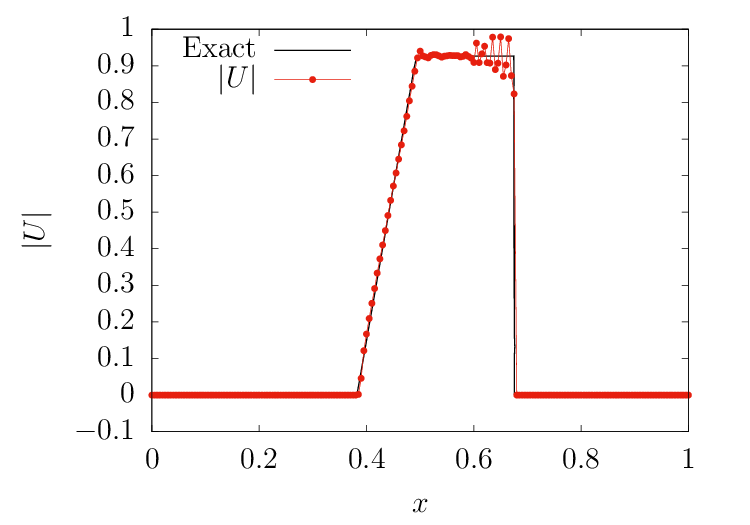
\includegraphics[width=0.45\linewidth]{Figures/Sod_umag_rcf}\\
		(c)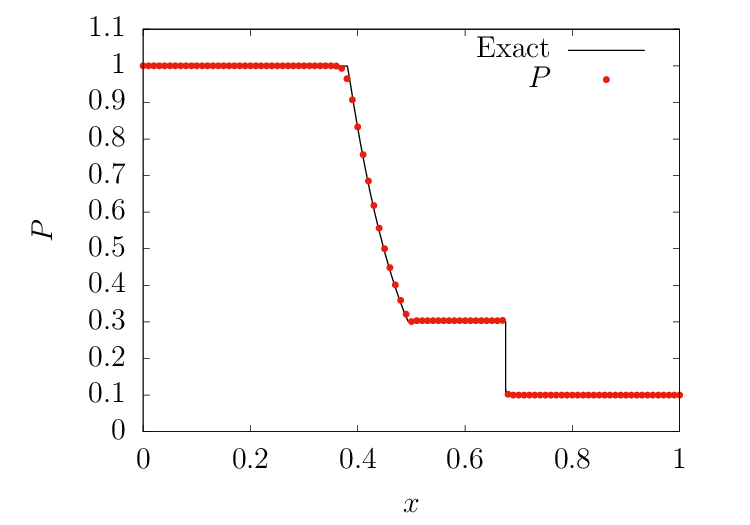
\includegraphics[width=0.45\linewidth]{Figures/Sod_p_ref}
		(d)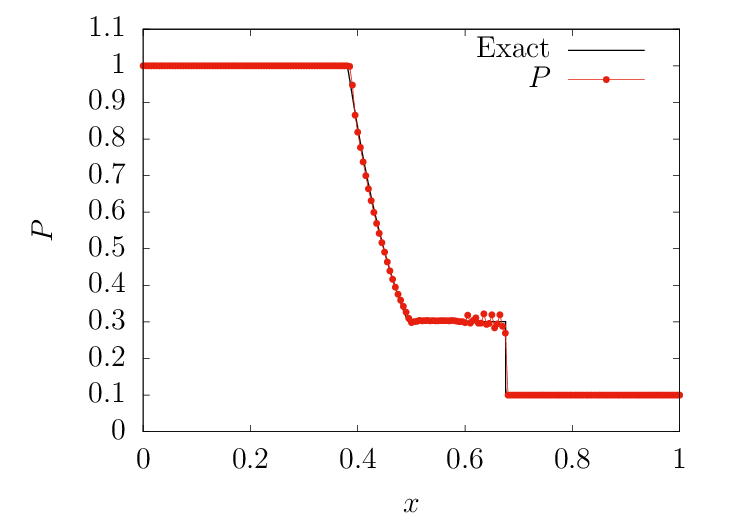
\includegraphics[width=0.45\linewidth]{Figures/Sod_p_rcf}\\
		(e)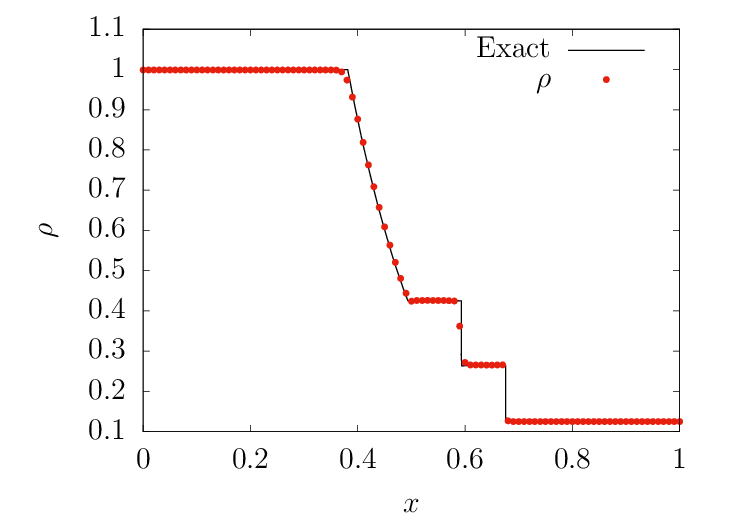
\includegraphics[width=0.45\linewidth]{Figures/Sod_rho_ref}
		(f)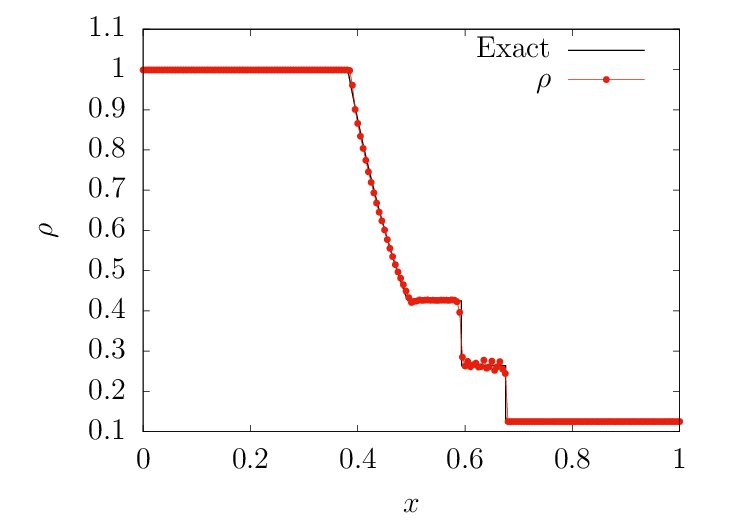
\includegraphics[width=0.45\linewidth]{Figures/Sod_rho_rcf}\\
		\caption[Velocity magnitude, Pressure and denisty plots for the Sod's shock tube case.]{Sod's shock tube: Comparison of numerical results from \texttt{rhoEnergyFoam}(panels (a),(c),(e)) and \texttt{rhoCentralFoam} (panels (b),(d),(f)) for Sod's shock tube problem. The black solid lines represent the exact analytical solution, while the red dot show the numerical results. (a) and (b) display the velocity magnitude, (c) and (d) show the pressure distribution, and (e) and (f) present the density profile.}
		\label{Sod_plots}
	\end{figure}  
	
	\noindent Figure (\ref{Sod_plots}) contains six plots comparing the results of \texttt{rhoEnergyFoam} and \texttt{rhoCentralFoam}, for the Sod's shock tube simulation. Plots (a) and (b) depict the velocity magnitude, (c) and (d) show the pressure distribution, while (e) and (f) present the density profile. The red dots represent the numerical results obtained from the solvers, while the black solid lines correspond to the exact analytical solution. From the comparison, it is evident that \texttt{rhoEnergyFoam} (plots a, c, and e) closely matches the exact solution with minimal deviation. In fact, it manages to capture the shock wave, rarefaction wave, and contact discontinuity accurately as well as the pressure drop across the shock and the density jump. In contrast, \texttt{rhoCentralFoam} (plots b, d, and f) exhibits noticeable discrepancies, particularly in the velocity and pressure profiles, where numerical oscillations appear around the discontinuities. This proves that \texttt{rhoEnergyFoam} provides a more accurate and stable solution for this type of problem, while \texttt{rhoCentralFoam} struggles to capture the shock and rarefaction waves correctly, becasue it exhibits oscillations around the shock and contact discontinuity.
	
	\newpage
	\section{Supersonic flow over a forward-facing step}
	The study of inviscid flow over a forward-facing step was originally introduced by \citet{EMERY1968306} to evaluate the effectiveness of shock-capturing schemes. In this work, this configuration is used to analyze the performance of \texttt{rhoEnergyFoam} in simulating supersonic flows in the presence of shock waves.
	
	\begin{figure}[h]
		\centering
		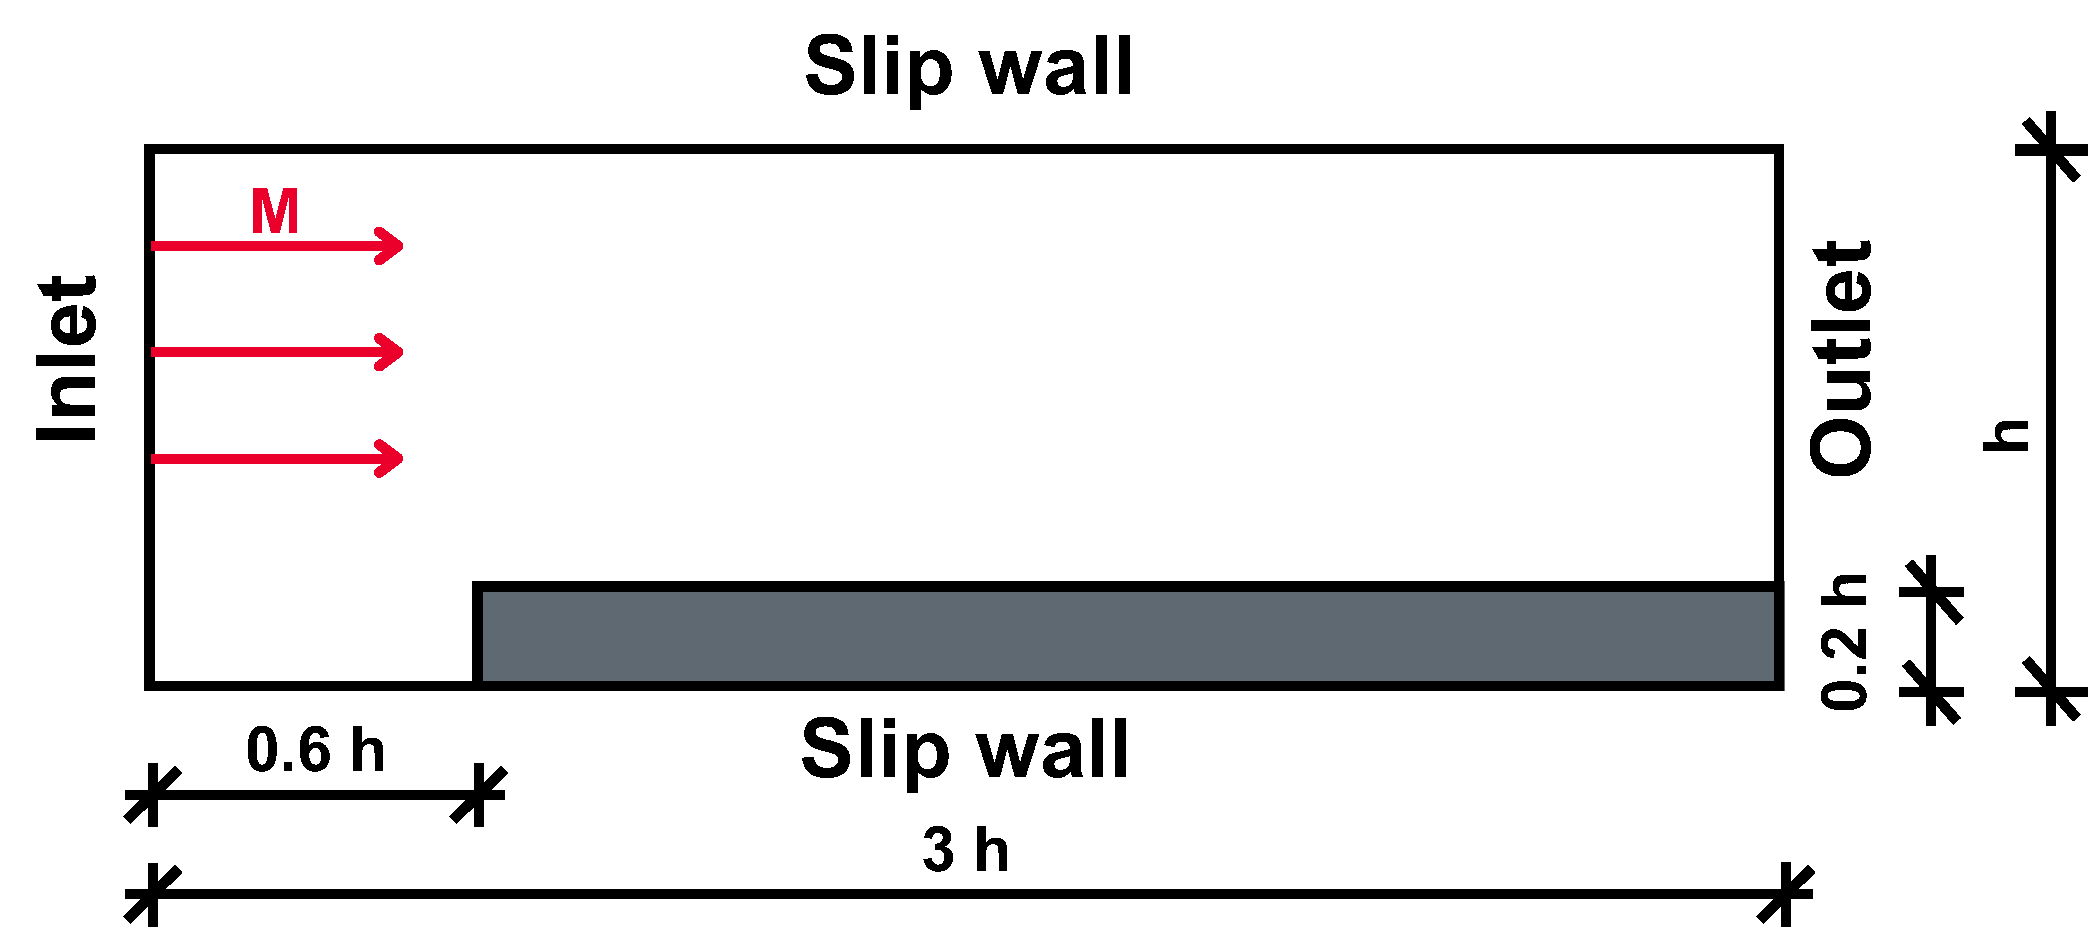
\includegraphics[width=0.7 \linewidth]{Figures/FS_Geometry}
		\caption{Geometry of the forward-facing step and its boundary conditions}
		\label{FS_Geometry}
	\end{figure} 
	
	\noindent The case considered involves a supersonic flow (Mach number $Ma = 3$) encountering a step of height $0.2\,h$, where $h$ represents the channel height, as shown in figure \ref{FS_Geometry}. The total channel length is $3\,h$, with the leading edge of the step positioned at $0.6\,h$ from the inlet. The spatial discretization is uniform, consisting of a grid with $240 \times 80$ cells along the coordinate directions. 	The thermodynamic properties of the gas considered are defined as follows: specific heat at constant volume: $C_v = 1.785$ J/kgK, the gas constant: $R = 0.714286$ J/kgK and thermal conductivity: $k = 32.3 \,\mu$W/mK. The boundary conditions include slip walls on the upper and lower surfaces, while all variables are extrapolated at the outlet. \\
	\\
	In detail:
	
	\begin{itemize}
		\item \textbf{Inlet} (left): fixed-value condition for velocity $U = 3$ m/s (Mach 3), pressure $p = 1$ Pa, and temperature $T = 1$ K;
		\item \textbf{Outlet} (right): \texttt{zeroGradient} condition on $U$, $p$, and $T$;
		\item \textbf{Bottom wall}: no-slip adiabatic wall condition;
		\item \textbf{Top wall}: symmetry plane condition.
	\end{itemize}
	
	\noindent The initial conditions for the simulation are: velocity  $U = 0$ m/s, pressure $p = 1$ Pa, and temperature: $T = 1$ K. The case is designed such that the speed of sound in the gas is	$c = \sqrt{\gamma R T} = 1 \text{ m/s}$. As a result, the velocity values are directly equivalent to the Mach number, meaning that an inlet velocity of 3 m/s corresponds to Mach 3.
	\\
	This speed of sound relation can be verified using the equation for a perfect gas which yields the specific heat ratio $\gamma = \frac{C_p}{C_v}$. 
	For this test case the solver is run in Mode C, with threshold
	value of the shock sensor $\theta^* = 0.05$ and $k_u = 0.25$, rather than the value suggested by \citet{LIOU_AUSM+-up}, as we observed a smoother shock front in this case.
	Analysis of the shock structure reveals that, although \texttt{rhoEnergyFoam} and \texttt{rhoCentralFOAM} produce qualitatively similar results as shown in figures (\ref{FS_ref}, \ref{FS_rcf}), \texttt{rhoEnergyFoam} provides additional flow details. In particular, the slip line emerging from the quadruple point near the upper wall is barely visible in \texttt{rhoCentralFOAM} due to its higher numerical diffusion.
	
	\begin{figure}[h]
		\centering
		\subfloat
		{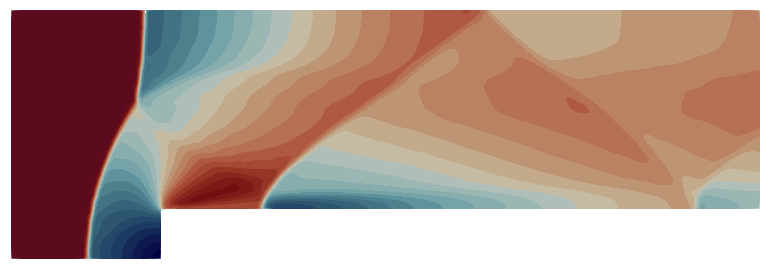
\includegraphics[width=0.7\textwidth]{Figures/FS_rcf}} \quad 
		\subfloat
		\centering
		{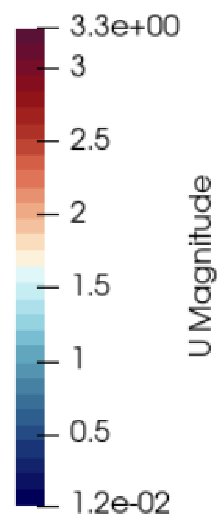
\includegraphics[width=0.1\textwidth, height=0.16\textheight]{Figures/FS_velocitybar}}
		\caption{rhoCentralFoam: supersonic flow past forward-facing step at $Ma = 3$.}
		\label{FS_rcf}
	\end{figure}
	
	\begin{figure}[h]
		\centering
		\subfloat
		{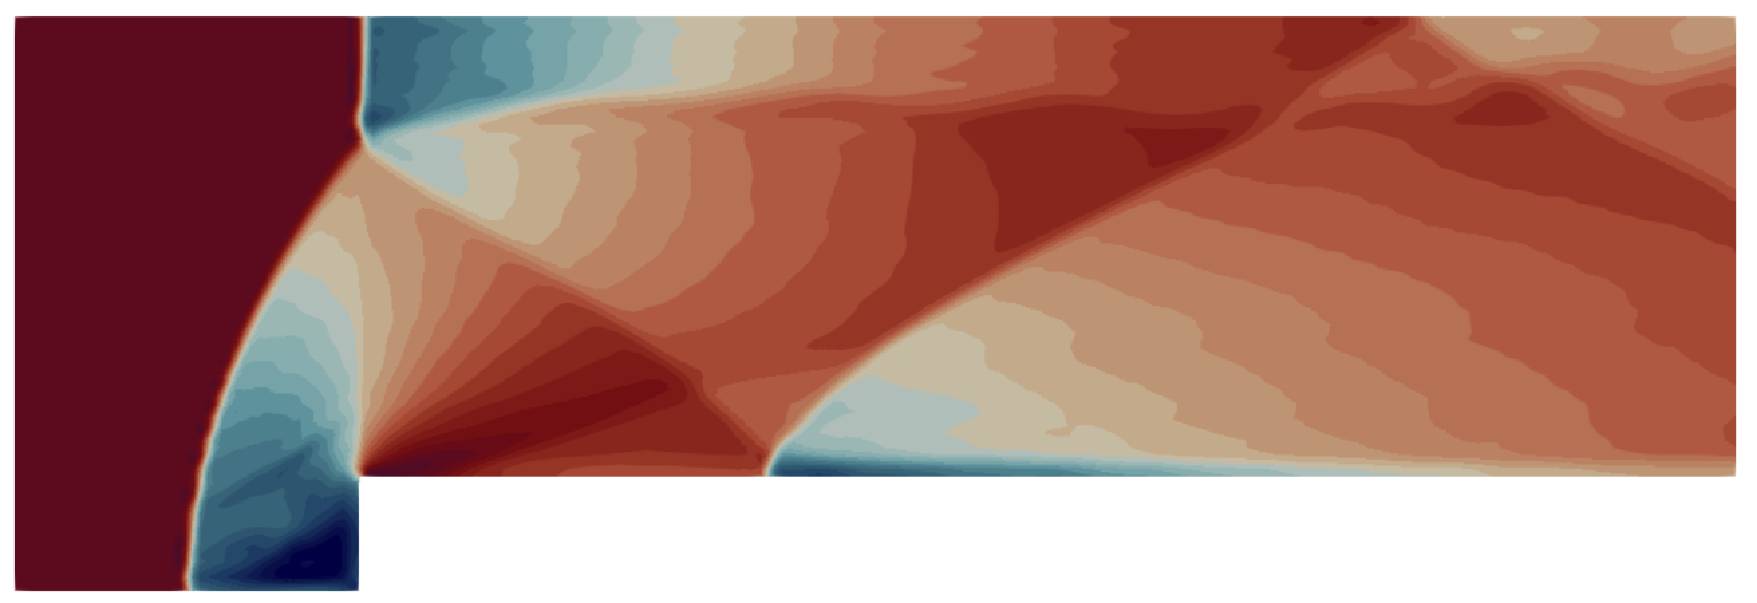
\includegraphics[width=0.7\textwidth]{Figures/FS_velocity}} \quad 
		\subfloat
		\centering
		{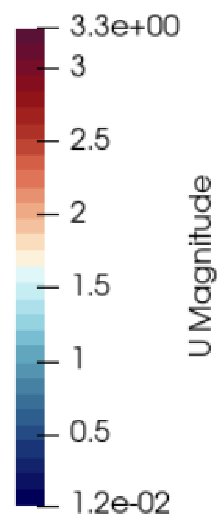
\includegraphics[width=0.1\textwidth, height=0.16\textheight]{Figures/FS_velocitybar}}
		\caption{rhoEnergyFoam: supersonic flow past forward-facing step at $Ma = 3$.}
		\label{FS_ref}
	\end{figure}
	
	\section{Transonic flow over RAE-2822 airfoil}
	The RAE-2822 airfoil is herein simulated by Reynolds-Averaged Navier-Stokes (RANS) equations, with both \texttt{rhoEnergyFoam} in mode C and \texttt{rhoCentralFoam}, using the standard Spalart-Allmaras model. The flow is transonic with a Mach number $M = 0.729$ and the Reynolds number of the chord considered is $Re_c = 6.5 \times 10^6$, defined as
	
	\begin{equation}
		Re_c = \frac{\rho_0 u_0 c}{\mu_0} 
	\end{equation}
	\\
	where $\rho_0$ is the density, $u_0$ is the initial velocity $c$ is the airfoil chord and $\mu_0$ is the dynamic viscosity. The angle of attack used to simulate the airfoil is $\alpha = 2.31^\circ$. A C-type structured mesh comprising $369 \times 256$ cells was used, with hyperbolic tangent extending toward the wall. The “farfield” boundary is located about 20 chords from the wall, where inlet/outlet boundary conditions are imposed, while isothermal nonslip boundary conditions are imposed on the airfoil wall.
	
	\begin{figure}[h]
		\centering
		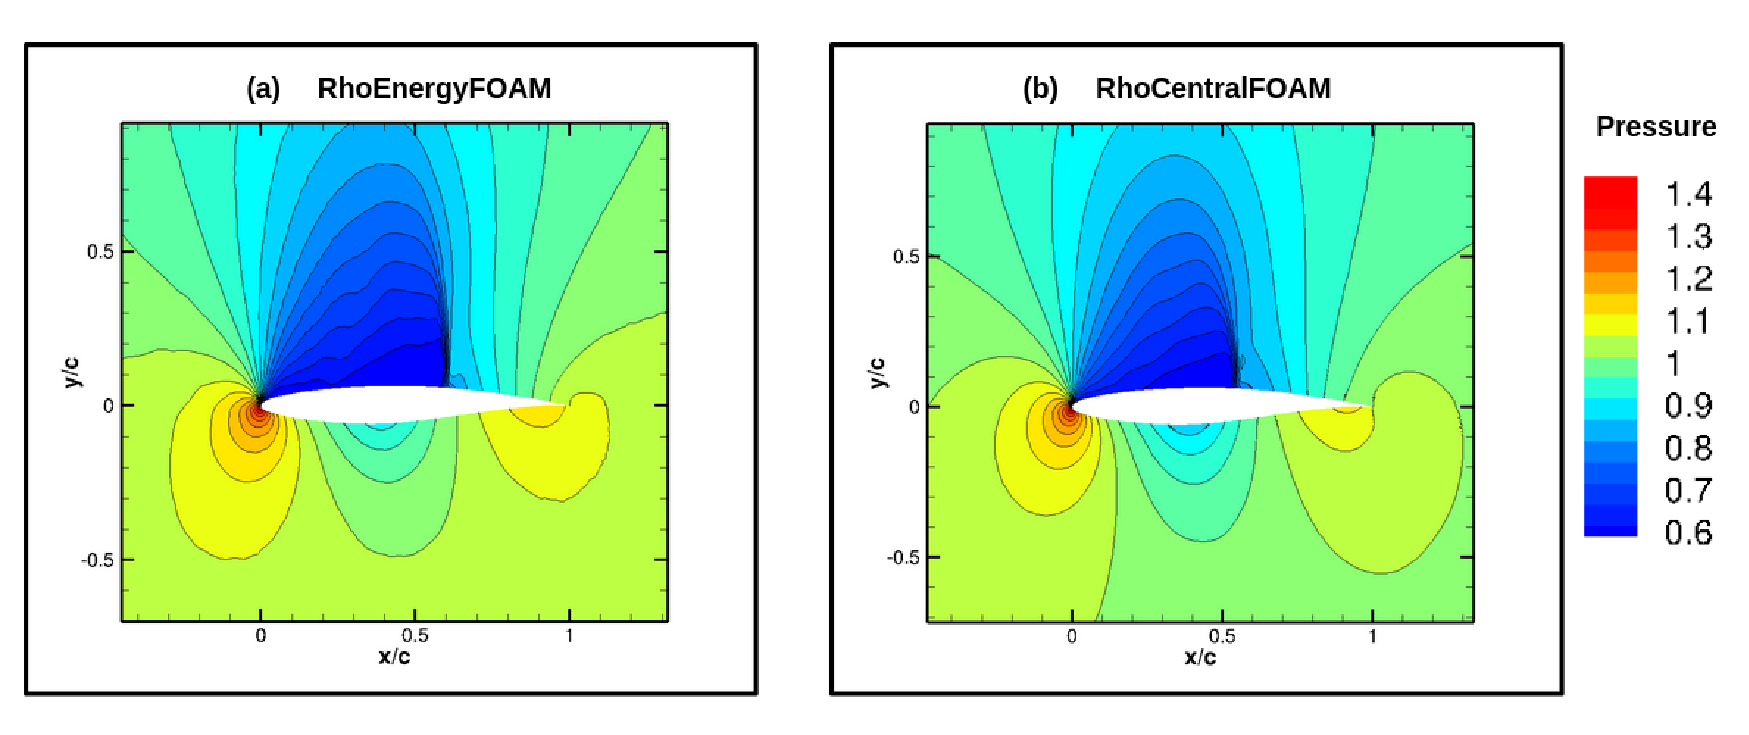
\includegraphics[width=1\textwidth]{Figures/RAE2822_pressurefield}
		\caption[Pressure field of a RANS of a transonic flow over RAE2822]{RANS of a transonic flow over RAE2822: Pressure fields evaluated with \texttt{rhoEnergyFoam} (a) and \texttt{rhoCentralFoam} (b). In the representation, 24 levels were used in the range  $0.6 < p/p_\infty < 1.4$.}
		\label{RAE2822_pressurefield}
	\end{figure}
	
	\noindent The calculated pressure fields are compared in figure (\ref{RAE2822_pressurefield}), which shows the presence of a single normal shock on the suction side and minimal differences between the two solvers. The detailed comparison of the pressure coefficients with the \citet{cook1977aerofoil} experiments and the \cite{slater2010rae2822} simulations, shown in figure (\ref{Cp_RAE2822}), is satisfactory for both solvers, although in this case \texttt{rhoCentralFoam} seems to be closer to the experiments and \texttt{rhoEnergyFoam} closer to the previous simulations. Finally we present table \ref{CLCDRAE2822} which shows the lift and
	drag coefficient predicted by the two solver.
	
	\begin{table}[h]
		\centering
		\begin{tabular}{lcc}
			\hline
			\textbf{Case} & $C_l$ & $C_d$ \\
			\hline
			\textit{rhoEnergyFoam}              & 0.715 & 0.0135 \\
			\textit{rhoCentralFoam}             & 0.730 & 0.0184 \\
			RANS \citep{coakley1987numerical}   & 0.717 & 0.0133 \\
			Experiment \citep{cook1977aerofoil} & 0.743 & 0.0127 \\
			\hline
		\end{tabular}
		\vspace{3mm}
		\caption[Lift and drag coefficient of RAE 2822 airfoil]{Lift and drag coefficient of RAE 2822 airfoil as predicted by rhoEnergyFoam and rhoCentralFoam, compared with \citet{coakley1987numerical} RANS and experimental data}
		\label{CLCDRAE2822}
	\end{table}
	
	\begin{figure}[h]
		\centering
		\begin{minipage}{0.62\textwidth}
			\centering
			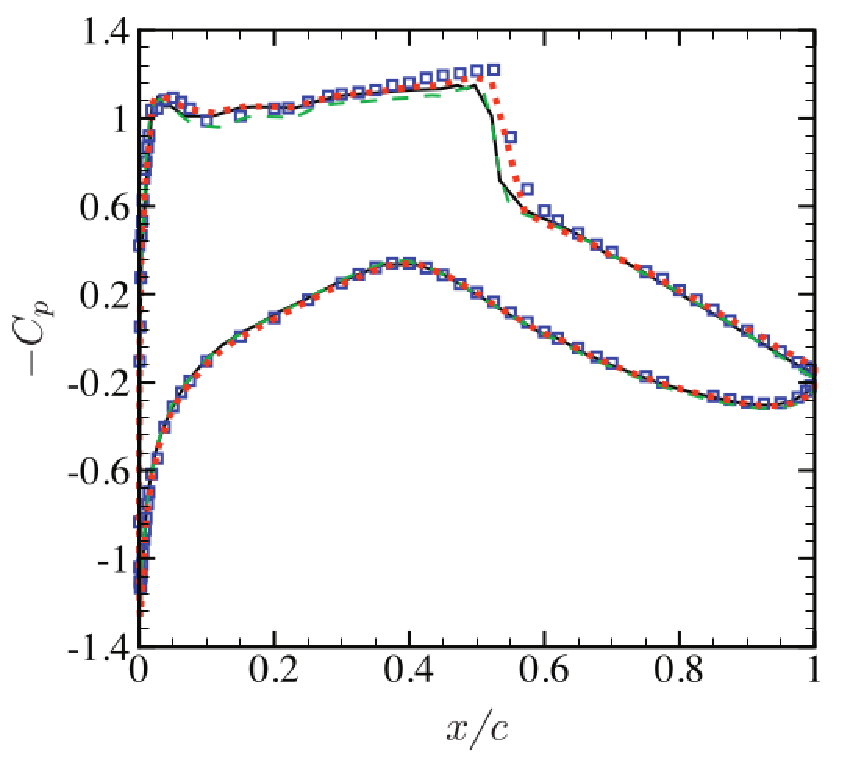
\includegraphics[width=1\textwidth, height=0.8\textwidth]{Figures/Cp_RAE2822}
		\end{minipage}
		\centering
		\begin{minipage}{0.8\textwidth}
			\centering
			\scriptsize
			\hspace{9mm}
			\begin{tabular}{cc}
				\toprule
				\textit{rhoEnergyFoam} &  \textcolor{red}{\rule{0.05\linewidth}{0.75mm}} \\
				\textit{rhoCentralFoam}  	   & 
				\textcolor{blue}{\rule{0.05\linewidth}{0.75mm}} \\
				RANS        &  \textcolor{green}{\rule{0.05\linewidth}{0.75mm}} \\
				Experiment        &  \textcolor{black}{\rule{0.05\linewidth}{0.75mm}} \\
				\bottomrule
			\end{tabular}
		\end{minipage}
			\caption[Pressure coefficient of RANS of a transonic flow over RAE2822]{RANS of a transonic flow over RAE2822: pressure coefficient obtained with \texttt{rhoEnergyFoam} (red line) and with \texttt{rhoCentralFoam} (blue dotted lines),compared with previous RANS (green crosses) and experimental data (black dotted lines).}
		\label{Cp_RAE2822}
	\end{figure}
	
				
	\newpage

	\section{Transonic flow over Onera M6 wing}
	This case aims to study the flow around the wing of Onera M6, whose flow is inviscid ($\mu_0$ = 0), transonic with Mach number $M = 0.8395$, and the angle of attack of the wing is $\alpha = 3.06^{\degree}$. An unstructured mesh including 341'797 tetrahedral cells was used, within an external computational box of size $L_x = 10c$, $L_y = 10c$ and $L_z = 5c$, where c is the chord in the wing root section, as shown in figure (\ref{OneraM6_mesh}). Numerical simulations were carried out using both \texttt{rhoCentralFoam} and \texttt{rhoEnergyFoam} in mode C, also comparing the results with experimental data values.
	
	\begin{figure}[h]
		\centering
		{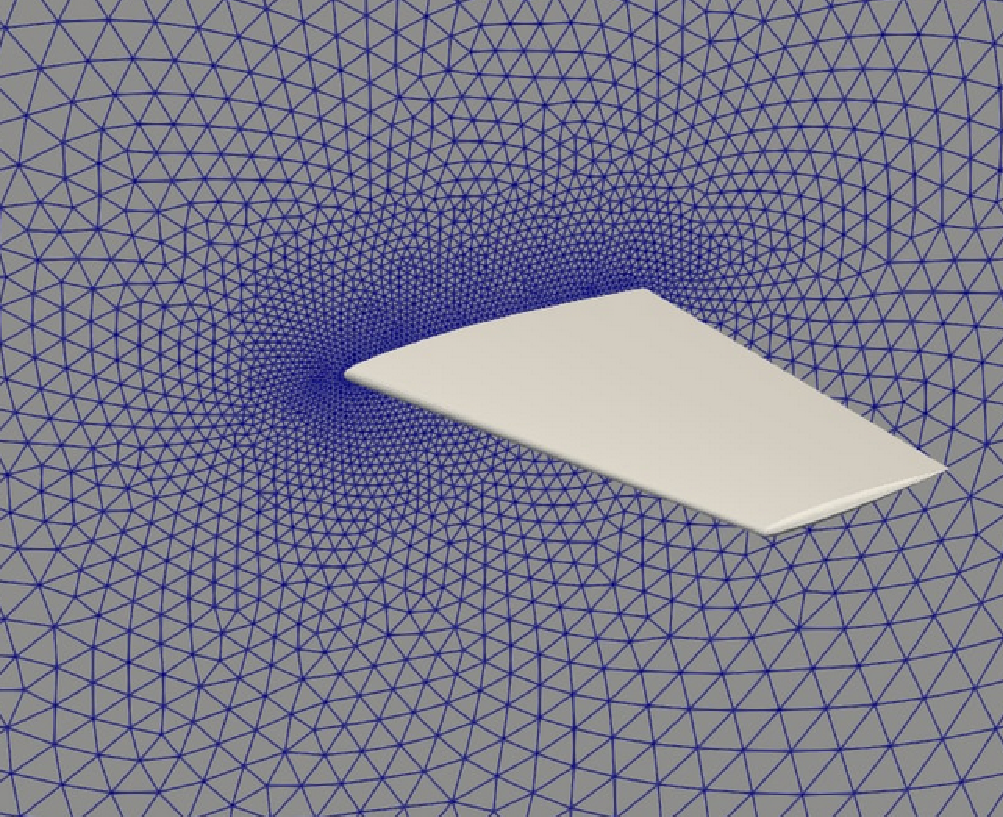
\includegraphics[width=0.6\linewidth]{Figures/OneraM6mesh}}  
		\caption[Unstructured mesh of the Onera M6 wing]{Unstructured mesh of the Onera M6 wing, within an external computational box of size $L_x = 10c$, $L_y = 10c$ and $L_z = 5c$, where c is the chord in the wing root section.}
		\label{OneraM6_mesh}
	\end{figure}
	
	\noindent Numerical simulations were carried out using \texttt{rhoCentralFoam} and \texttt{rhoEnergyFoam} in mode C, also comparing the results with experimental data values. Figure (\ref{OneraM6_pressurefield}) shows the pressure field obtained with \texttt{rhoEnergyFoam}, plotting the isosurface of the shock sensor over it, showing the presence of two shock waves: the main shock about halfway up the chord and a secondary shock near the leading edge, which eventually join near the wing tip.
	
	\begin{figure}[h]
		\centering
		{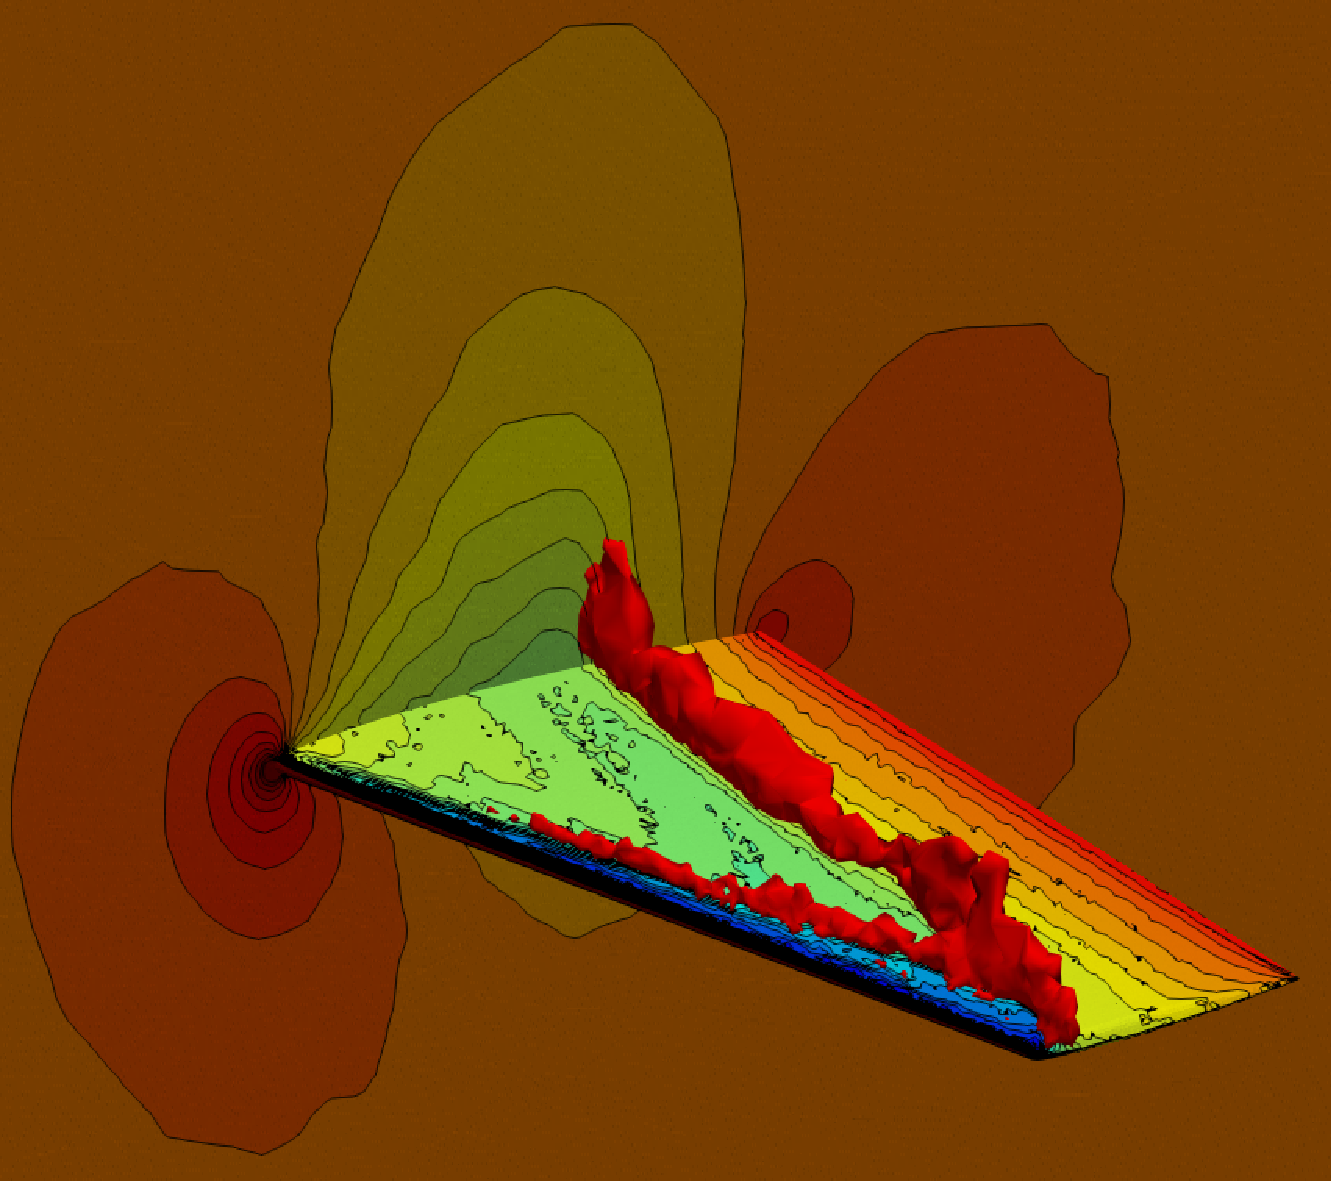
\includegraphics[width=0.7\linewidth, height=0.35\textheight]{Figures/Ducros}}  \\
		\centering
		{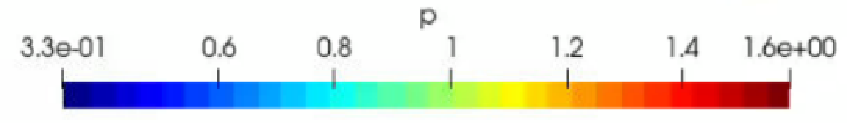
\includegraphics[width=0.6\linewidth]{Figures/Ducros_bar}}
		\caption[Pressure field Onera M6]{Pressure field with Ducros sensor isosurface superimposed ($\theta = 0.6$), showing the presence of two shock waves, of the Onera M6 wing. In the representation, 24 levels were used in the range  $0.33 < p/p_\infty < 1.6$.}
		\label{OneraM6_pressurefield}
	\end{figure}
	
	\noindent Figure (\ref{Cp_contours_oneraM6}) shows the calculated pressure field on the wing suction surface for \texttt{rhoEnergyFoam} (figure \ref{Cp_contours_oneraM6}a) and rhoCentralFoam (figure \ref{Cp_contours_oneraM6}b), which highlights the qualitative differences between the two solvers.
	
	\begin{figure}[t]
		\centering
		(a)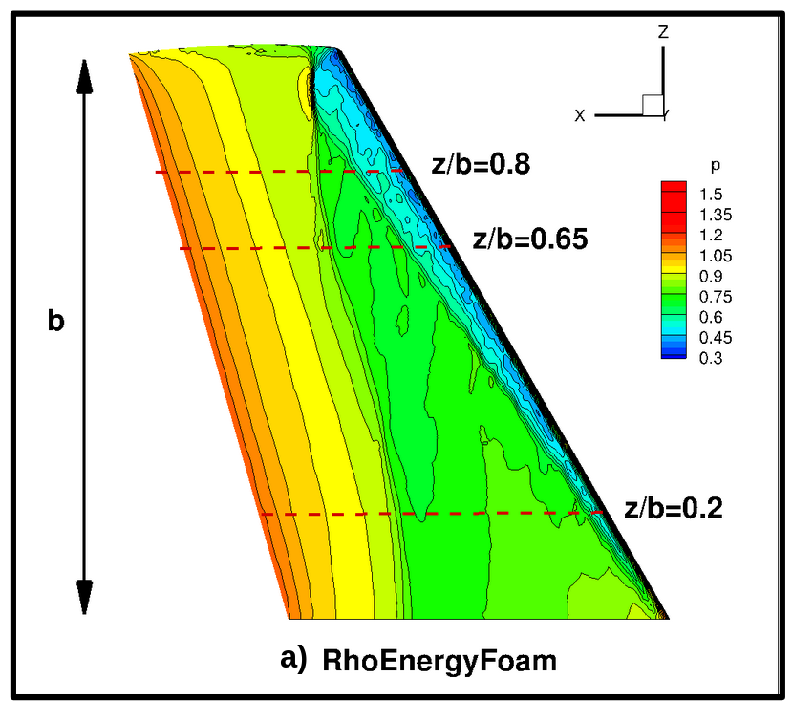
\includegraphics[width=0.45\linewidth]{Figures/Cp_contours_oneram6_ref}
		(b)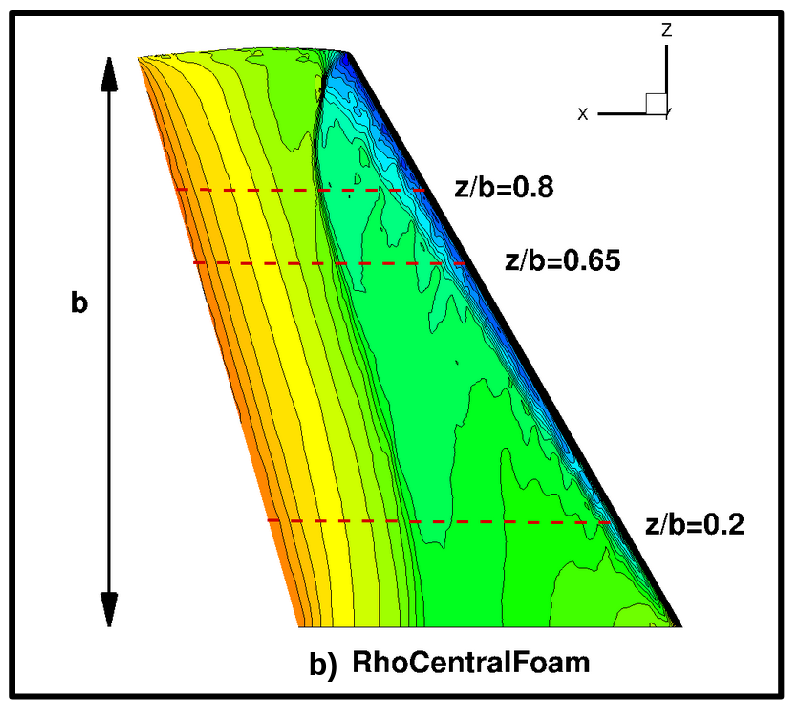
\includegraphics[width=0.45\linewidth]{Figures/Cp_contours_oneram6_rcf}
		\caption[Pressure field of a flow around Onera M6 wing]{Flow around the wing of ONERA M6: pressure profiles evaluated with \texttt{rhoEnergyFoam} (a) and \texttt{rhoCentralFoam} (b). In range $0.3 < p/p_\infty < 1.5$ are shown 32 levels  (blue-to-red scale). Dotted lines point to section used to evaluate pressure coefficients as in \ref{Cp_oneraM6}}
		\label{Cp_contours_oneraM6}
	\end{figure}
	
	 \noindent Although the main flow characteristics are captured by both of them, it appears that the edge shock is much weaker in rhoCentralFoam and the primary shock is much thicker, especially toward the wing root, due to the diffusive nature of the solver. A more quantitative assessment is made in figure (\ref{Cp_oneraM6}), where the calculated distributions of the pressure coefficient are compared with \citet{schmitt1979pressure} experimental data, at the three wing sections indicated by the dashed lines in Figure (\ref{Cp_contours_oneraM6}). In the innermost section (panel a) the primary shock is rather weak and barely noticeable in \texttt{rhoCentralFoam}, while \texttt{rhoEnergyFoam} provides a favorable prediction of both the strength and position of the shock. In the second section (panels b) there are both shocks, which are again correctly captured by \texttt{rhoEnergyFoam}, while \texttt{rhoCentralFoam} shows excessive smearing. In the outermost section (panel c) the primary and secondary shocks merge into a single stronger shock, the amplitude of which is well captured by \texttt{rhoEnergyFoam}. 
	
	\begin{figure}[h]
		\begin{center}
			(a)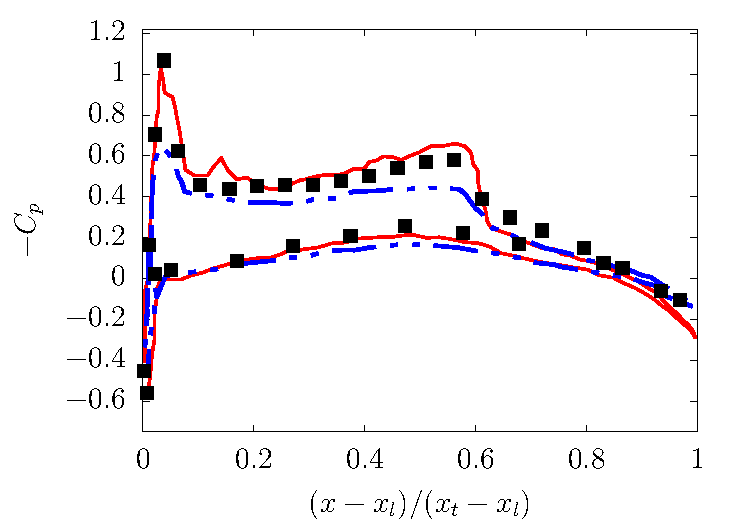
\includegraphics[width=0.45\linewidth]{Figures/Cp_oneram6_02}
			(b)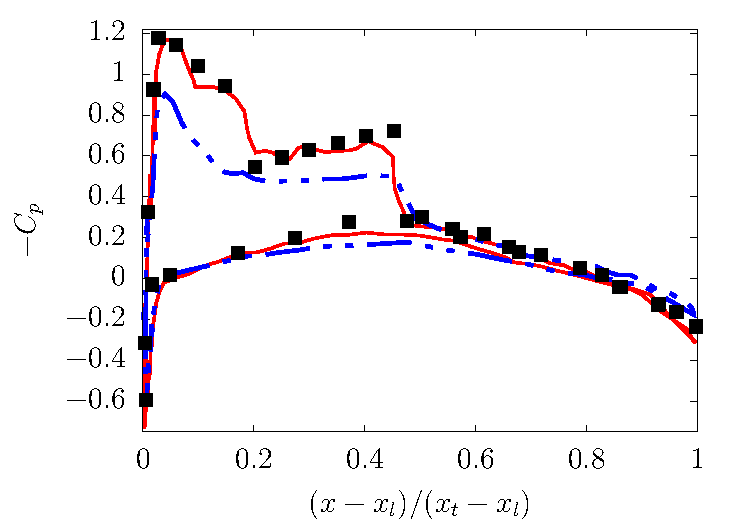
\includegraphics[width=0.45\linewidth]{Figures/Cp_oneram6_065}\\
			\vspace{3mm}
			(c)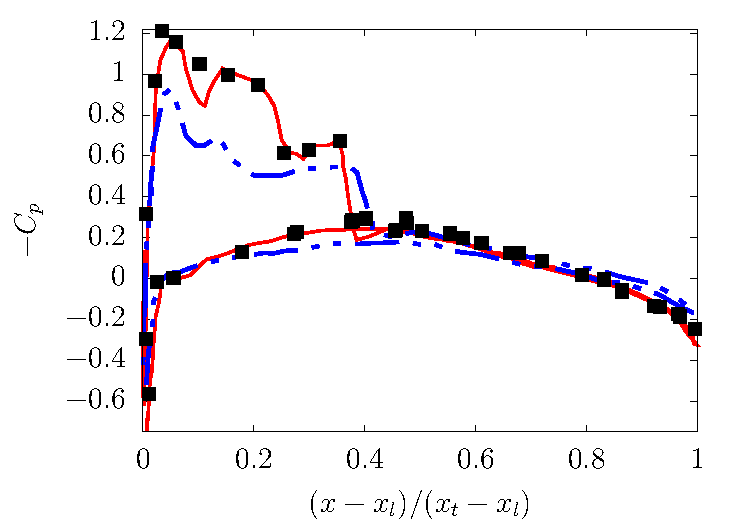
\includegraphics[width=0.45\linewidth]{Figures/Cp_oneram6_08}
			\caption[Pressure coefficient of the flow around ONERA M6 wing.]{Flow around ONERA M6 wing: pressure coefficient $(Cp = (p-p_\infty)/(\dfrac{1}{2}\rho_\infty u^2_\infty))$ at various wing sections: (a) $z/b = 0.2$, (b) $z/b = 0.65$ and (c) $z/b = 0.8$, for rhoEnergyFoam (red lines), rhoCentralFoam (blue dotted lines) and experimental data (black squares). $x_l$ and $x_t$ denote the coordinates of the leading edge and trailing edge of each wing section, respectively.}
			\label{Cp_oneraM6}
		\end{center}
	\end{figure}
	
	\chapter{Conclusion and Future Development}
	\label{chap:conclusion}
	
	The development of the \texttt{rhoEnergyFoam} solver represents a significant advancement in the numerical simulation of compressible turbulent flows. By leveraging an energy-consistent, non-diffusive numerical flux and selectively incorporating diffusion based on flow characteristics, the solver effectively balances accuracy and stability. The introduction of a triple splitting approach, previously unexplored in finite-volume methods, and the decomposition of the AUSM diffusive flux into distinct pressure and convective components ensure minimal numerical dissipation while maintaining robustness. The three-mode operational framework provides tailored numerical diffusion for different flow regimes: fully resolved simulations (Mode A) operate without artificial diffusion, unresolved smooth flows (Mode B) utilize minimal pressure diffusion, and shocked flows (Mode C) employ both pressure and convective diffusion to enhance stability.
	\\
	Implemented within the OpenFOAM framework, \texttt{rhoEnergyFoam} has demonstrated superior performance across a spectrum of test cases, from canonical turbulence problems to applied aerodynamic flows. It significantly outperforms standard OpenFOAM solvers in preserving kinetic energy, a crucial feature for unsteady RANS and Large Eddy Simulation (LES), thereby improving turbulence accuracy and aerodynamic force predictions. This reduction in numerical diffusion ensures that turbulence structures are preserved without unnecessary dissipation, addressing a common drawback of traditional schemes. The ability to retain energy fidelity in turbulence simulations is essential for accurately capturing flow physics, making \texttt{rhoEnergyFoam} a valuable tool for high-resolution CFD applications.
	\\
	A key advantage of \texttt{rhoEnergyFoam} is its ability to accurately capture shock phenomena while minimizing numerical diffusion. By selectively applying AUSM pressure and convective diffusive fluxes based on a local shock sensor, the solver avoids excessive dissipation, ensuring sharp resolution of shocks while maintaining stability. This capability is particularly relevant for aerospace and automotive applications, where capturing shocks in supersonic flows simulations is crucial for aerodynamic performance. Traditional solvers often struggle to achieve this balance, leading to either excessive numerical damping that compromises accuracy or unstable solutions that necessitate additional artificial dissipation. \texttt{rhoEnergyFoam} mitigates these issues by dynamically adjusting diffusion, allowing it to operate efficiently across a broad range of Mach and Reynolds numbers.
	\\
	The open-source nature of the solver fosters collaboration and further development within the CFD community. Open-source accessibility encourages customization, improvement, and widespread adoption, bridging the gap between specialized high-accuracy numerical methods and general-purpose CFD solvers. This makes \texttt{rhoEnergyFoam} a valuable tool for both academic research and industrial applications. By providing an accessible platform for innovation, the solver enables users to develop new numerical techniques, optimize turbulence models, and expand its applicability to complex engineering challenges.
	\\
	Moreover, the solver’s ability to maintain accuracy on unstructured meshes without requiring excessive artificial diffusion enhances its usability in industrial settings, where complex geometries and varying grid resolutions are common. The incorporation of low-dissipative numerics ensures that intricate flow structures are retained even in highly turbulent environments. This feature is particularly useful in engineering disciplines such as aerodynamics, propulsion, and energy systems, where accurate flow predictions are essential for optimizing design and performance.
	\\
	In conclusion, \texttt{rhoEnergyFoam} provides a powerful, low-dissipation, energy-preserving approach for high-fidelity CFD simulations. Its integration within OpenFOAM enhances accessibility, while its innovative numerical strategies improve accuracy and stability across a wide range of flow problems. Through continued development and adoption, \texttt{rhoEnergyFoam} has the potential to reshape computational fluid dynamics, enabling more efficient and precise simulations for engineering applications. As a future step, GPU acceleration could significantly enhance computational efficiency, reducing turnaround times for large-scale simulations and further broadening its industrial applicability. Implementing a GPU-accelerated version of \texttt{rhoEnergyFoam} would allow for larger simulations to be performed at unprecedented speeds, facilitating real-time analysis and optimization in engineering workflows. This advancement would make high-fidelity simulations more practical for time-sensitive applications, reinforcing the solver’s role as a next-generation CFD tool.
	
	\newpage

	%\backmatter
	%\cleardoublepage
	\phantomsection % Give this command only if hyperref is loaded
	\addcontentsline{toc}{chapter}{\bibname}
	% Here put the code for the bibliography. You can use BibTeX or
	% the BibLaTeX package or the simple environment thebibliography.
		% References
	\bibliography{references.bib}  % 'references.bib' file 
	%for the bibliography
	%\printbibliography[heading=bibintoc]
	

\end{document}
